% **************************************************************************************************************
% A Classic Thesis Style
% An Homage to The Elements of Typographic Style
%
% Copyright (C) 2015 André Miede http://www.miede.de
%
% If you like the style then I would appreciate a postcard. My address 
% can be found in the file ClassicThesis.pdf. A collection of the 
% postcards I received so far is available online at 
% http://postcards.miede.de
%
% License:
% This program is free software; you can redistribute it and/or modify
% it under the terms of the GNU General Public License as published by
% the Free Software Foundation; either version 2 of the License, or
% (at your option) any later version.
%
% This program is distributed in the hope that it will be useful,
% but WITHOUT ANY WARRANTY; without even the implied warranty of
% MERCHANTABILITY or FITNESS FOR A PARTICULAR PURPOSE.  See the
% GNU General Public License for more details.
%
% You should have received a copy of the GNU General Public License
% along with this program; see the file COPYING.  If not, write to
% the Free Software Foundation, Inc., 59 Temple Place - Suite 330,
% Boston, MA 02111-1307, USA.
%
% **************************************************************************************************************
\RequirePackage{fix-cm} % fix some latex issues see: http://texdoc.net/texmf-dist/doc/latex/base/fixltx2e.pdf
\documentclass[ twoside,openright,titlepage,numbers=noenddot,headinclude,%1headlines,% letterpaper a4paper
                footinclude=true,cleardoublepage=empty,abstractoff, % <--- obsolete, remove (todo)
                BCOR=5mm,paper=a4,fontsize=11pt,%11pt,a4paper,%
                ngerman,american,%
                ]{scrreprt}

%********************************************************************
% Note: Make all your adjustments in here
%*******************************************************
% ****************************************************************************************************
% classicthesis-config.tex 
% formerly known as loadpackages.sty, classicthesis-ldpkg.sty, and classicthesis-preamble.sty 
% Use it at the beginning of your ClassicThesis.tex, or as a LaTeX Preamble 
% in your ClassicThesis.{tex,lyx} with % ****************************************************************************************************
% classicthesis-config.tex 
% formerly known as loadpackages.sty, classicthesis-ldpkg.sty, and classicthesis-preamble.sty 
% Use it at the beginning of your ClassicThesis.tex, or as a LaTeX Preamble 
% in your ClassicThesis.{tex,lyx} with % ****************************************************************************************************
% classicthesis-config.tex 
% formerly known as loadpackages.sty, classicthesis-ldpkg.sty, and classicthesis-preamble.sty 
% Use it at the beginning of your ClassicThesis.tex, or as a LaTeX Preamble 
% in your ClassicThesis.{tex,lyx} with \input{classicthesis-config}
% ****************************************************************************************************  
% If you like the classicthesis, then I would appreciate a postcard. 
% My address can be found in the file ClassicThesis.pdf. A collection 
% of the postcards I received so far is available online at 
% http://postcards.miede.de
% ****************************************************************************************************


% ****************************************************************************************************
% 0. Set the encoding of your files. UTF-8 is the only sensible encoding nowadays. If you can't read
% äöüßáéçèê∂åëæƒÏ€ then change the encoding setting in your editor, not the line below. If your editor
% does not support utf8 use another editor!
% ****************************************************************************************************
\PassOptionsToPackage{utf8}{inputenc}
	\usepackage{inputenc}

% ****************************************************************************************************
% 1. Configure classicthesis for your needs here, e.g., remove "drafting" below 
% in order to deactivate the time-stamp on the pages
% ****************************************************************************************************
\PassOptionsToPackage{eulerchapternumbers,listings,%
					 pdfspacing,floatperchapter,%linedheaders,%
					 subfig,beramono,eulermath}{classicthesis}                                        
% ********************************************************************
% Available options for classicthesis.sty 
% (see ClassicThesis.pdf for more information):
% drafting
% parts nochapters linedheaders
% eulerchapternumbers beramono eulermath pdfspacing minionprospacing
% tocaligned dottedtoc manychapters
% listings floatperchapter subfig
% ********************************************************************


% ****************************************************************************************************
% 2. Personal data and user ad-hoc commands
% ****************************************************************************************************
\newcommand{\myTitle}{Black hole masses and outflows in high redshift quasars\xspace}
\newcommand{\mySubtitle}{An Homage to The Elements of Typographic Style\xspace}
\newcommand{\myDegree}{Doktor-Ingenieur (Dr.-Ing.)\xspace}
\newcommand{\myName}{Liam Coatman\xspace}
\newcommand{\myProf}{Put name here\xspace}
\newcommand{\myOtherProf}{Put name here\xspace}
\newcommand{\mySupervisor}{Put name here\xspace}
\newcommand{\myFaculty}{Put data here\xspace}
\newcommand{\myDepartment}{Put data here\xspace}
\newcommand{\myUni}{Put data here\xspace}
\newcommand{\myLocation}{Saarbrücken\xspace}
\newcommand{\myTime}{September 2015\xspace}
\newcommand{\myVersion}{version 4.2\xspace}

% ********************************************************************
% Setup, finetuning, and useful commands
% ********************************************************************
\newcounter{dummy} % necessary for correct hyperlinks (to index, bib, etc.)
\newlength{\abcd} % for ab..z string length calculation
\providecommand{\mLyX}{L\kern-.1667em\lower.25em\hbox{Y}\kern-.125emX\@}
\newcommand{\ie}{i.\,e.}
\newcommand{\Ie}{I.\,e.}
\newcommand{\eg}{e.\,g.}
\newcommand{\Eg}{E.\,g.} 
% ****************************************************************************************************


% ****************************************************************************************************
% 3. Loading some handy packages
% ****************************************************************************************************
% ******************************************************************** 
% Packages with options that might require adjustments
% ******************************************************************** 
%\PassOptionsToPackage{ngerman,american}{babel}   % change this to your language(s)
% Spanish languages need extra options in order to work with this template
%\PassOptionsToPackage{spanish,es-lcroman}{babel}
	\usepackage{babel}                  

\usepackage{csquotes}
\PassOptionsToPackage{%
    %backend=biber, %instead of bibtex
	backend=bibtex8,bibencoding=ascii,%
	language=auto,%
	% style=numeric-comp,%
    style=authoryear, % Author 1999, 2010
    % bibstyle=authoryear,dashed=false, % dashed: substitute rep. author with ---
    sorting=nyt, % name, year, title
    maxbibnames=10, % default: 3, et al.
    %backref=true,%
    natbib=true % natbib compatibility mode (\citep and \citet still work)
}{biblatex}
    \usepackage{biblatex}

\PassOptionsToPackage{fleqn}{amsmath}       % math environments and more by the AMS 
    \usepackage{amsmath}

% ******************************************************************** 
% General useful packages
% ******************************************************************** 
\PassOptionsToPackage{T1}{fontenc} % T2A for cyrillics
    \usepackage{fontenc}     
\usepackage{textcomp} % fix warning with missing font shapes
\usepackage{scrhack} % fix warnings when using KOMA with listings package          
\usepackage{xspace} % to get the spacing after macros right  
\usepackage{mparhack} % get marginpar right
\usepackage{fixltx2e} % fixes some LaTeX stuff --> since 2015 in the LaTeX kernel (see below)
%\usepackage[latest]{latexrelease} % will be used once available in more distributions (ISSUE #107)
\PassOptionsToPackage{printonlyused,smaller}{acronym} 
    \usepackage{acronym} % nice macros for handling all acronyms in the thesis
    %\renewcommand{\bflabel}[1]{{#1}\hfill} % fix the list of acronyms --> no longer working
    %\renewcommand*{\acsfont}[1]{\textsc{#1}} 
    \renewcommand*{\aclabelfont}[1]{\acsfont{#1}}
% ****************************************************************************************************


% ****************************************************************************************************
% 4. Setup floats: tables, (sub)figures, and captions
% ****************************************************************************************************
\usepackage{tabularx} % better tables
    \setlength{\extrarowheight}{3pt} % increase table row height
\newcommand{\tableheadline}[1]{\multicolumn{1}{c}{\spacedlowsmallcaps{#1}}}
\newcommand{\myfloatalign}{\centering} % to be used with each float for alignment
\usepackage{caption}
% Thanks to cgnieder and Claus Lahiri
% http://tex.stackexchange.com/questions/69349/spacedlowsmallcaps-in-caption-label
% [REMOVED DUE TO OTHER PROBLEMS, SEE ISSUE #82]    
%\DeclareCaptionLabelFormat{smallcaps}{\bothIfFirst{#1}{~}\MakeTextLowercase{\textsc{#2}}}
%\captionsetup{font=small,labelformat=smallcaps} % format=hang,
\captionsetup{font=small} % format=hang,
\usepackage{subfig}  
% ****************************************************************************************************


% ****************************************************************************************************
% 5. Setup code listings
% ****************************************************************************************************
\usepackage{listings} 
%\lstset{emph={trueIndex,root},emphstyle=\color{BlueViolet}}%\underbar} % for special keywords
\lstset{language=[LaTeX]Tex,%C++,
    morekeywords={PassOptionsToPackage,selectlanguage},
    keywordstyle=\color{RoyalBlue},%\bfseries,
    basicstyle=\small\ttfamily,
    %identifierstyle=\color{NavyBlue},
    commentstyle=\color{Green}\ttfamily,
    stringstyle=\rmfamily,
    numbers=none,%left,%
    numberstyle=\scriptsize,%\tiny
    stepnumber=5,
    numbersep=8pt,
    showstringspaces=false,
    breaklines=true,
    %frameround=ftff,
    %frame=single,
    belowcaptionskip=.75\baselineskip
    %frame=L
} 
% ****************************************************************************************************             


% ****************************************************************************************************
% 6. PDFLaTeX, hyperreferences and citation backreferences
% ****************************************************************************************************
% ********************************************************************
% Using PDFLaTeX
% ********************************************************************
\PassOptionsToPackage{pdftex,hyperfootnotes=false,pdfpagelabels}{hyperref}
    \usepackage{hyperref}  % backref linktocpage pagebackref
\pdfcompresslevel=9
\pdfadjustspacing=1 
\PassOptionsToPackage{pdftex}{graphicx}
    \usepackage{graphicx} 
 

% ********************************************************************
% Hyperreferences
% ********************************************************************
\hypersetup{%
    %draft, % = no hyperlinking at all (useful in b/w printouts)
    colorlinks=true, linktocpage=true, pdfstartpage=3, pdfstartview=FitV,%
    % uncomment the following line if you want to have black links (e.g., for printing)
    %colorlinks=false, linktocpage=false, pdfstartpage=3, pdfstartview=FitV, pdfborder={0 0 0},%
    breaklinks=true, pdfpagemode=UseNone, pageanchor=true, pdfpagemode=UseOutlines,%
    plainpages=false, bookmarksnumbered, bookmarksopen=true, bookmarksopenlevel=1,%
    hypertexnames=true, pdfhighlight=/O,%nesting=true,%frenchlinks,%
    urlcolor=RoyalBlue, linkcolor=RoyalBlue, citecolor=RoyalBlue, %pagecolor=RoyalBlue,%
    %urlcolor=Black, linkcolor=Black, citecolor=Black, %pagecolor=Black,%
    pdftitle={\myTitle},%
    pdfauthor={\textcopyright\ \myName, \myUni, \myFaculty},%
    pdfsubject={},%
    pdfkeywords={},%
    pdfcreator={pdfLaTeX},%
    pdfproducer={LaTeX with hyperref and classicthesis}%
}   

% ********************************************************************
% Setup autoreferences
% ********************************************************************
% There are some issues regarding autorefnames
% http://www.ureader.de/msg/136221647.aspx
% http://www.tex.ac.uk/cgi-bin/texfaq2html?label=latexwords
% you have to redefine the makros for the 
% language you use, e.g., american, ngerman
% (as chosen when loading babel/AtBeginDocument)
% ********************************************************************
\makeatletter
\@ifpackageloaded{babel}%
    {%
       \addto\extrasamerican{%
			\renewcommand*{\figureautorefname}{Figure}%
			\renewcommand*{\tableautorefname}{Table}%
			\renewcommand*{\partautorefname}{Part}%
			\renewcommand*{\chapterautorefname}{Chapter}%
			\renewcommand*{\sectionautorefname}{Section}%
			\renewcommand*{\subsectionautorefname}{Section}%
			\renewcommand*{\subsubsectionautorefname}{Section}%     
                }%
       \addto\extrasngerman{% 
			\renewcommand*{\paragraphautorefname}{Absatz}%
			\renewcommand*{\subparagraphautorefname}{Unterabsatz}%
			\renewcommand*{\footnoteautorefname}{Fu\"snote}%
			\renewcommand*{\FancyVerbLineautorefname}{Zeile}%
			\renewcommand*{\theoremautorefname}{Theorem}%
			\renewcommand*{\appendixautorefname}{Anhang}%
			\renewcommand*{\equationautorefname}{Gleichung}%        
			\renewcommand*{\itemautorefname}{Punkt}%
                }%  
            % Fix to getting autorefs for subfigures right (thanks to Belinda Vogt for changing the definition)
            \providecommand{\subfigureautorefname}{\figureautorefname}%             
    }{\relax}
\makeatother


% ****************************************************************************************************
% 7. Last calls before the bar closes
% ****************************************************************************************************
% ********************************************************************
% Development Stuff
% ********************************************************************
\listfiles
%\PassOptionsToPackage{l2tabu,orthodox,abort}{nag}
%   \usepackage{nag}
%\PassOptionsToPackage{warning, all}{onlyamsmath}
%   \usepackage{onlyamsmath}

% ********************************************************************
% Last, but not least...
% ********************************************************************
\usepackage{classicthesis} 
% ****************************************************************************************************


% ****************************************************************************************************
% 8. Further adjustments (experimental)
% ****************************************************************************************************
% ********************************************************************
% Changing the text area
% ********************************************************************
%\linespread{1.05} % a bit more for Palatino
%\areaset[current]{312pt}{761pt} % 686 (factor 2.2) + 33 head + 42 head \the\footskip
%\setlength{\marginparwidth}{7em}%
%\setlength{\marginparsep}{2em}%

% ********************************************************************
% Using different fonts
% ********************************************************************
%\usepackage[oldstylenums]{kpfonts} % oldstyle notextcomp
%\usepackage[osf]{libertine}
%\usepackage[light,condensed,math]{iwona}
%\renewcommand{\sfdefault}{iwona}
%\usepackage{lmodern} % <-- no osf support :-(
%\usepackage{cfr-lm} % 
%\usepackage[urw-garamond]{mathdesign} <-- no osf support :-(
%\usepackage[default,osfigures]{opensans} % scale=0.95 
%\usepackage[sfdefault]{FiraSans}
% ****************************************************************************************************

% ****************************************************************************************************  
% If you like the classicthesis, then I would appreciate a postcard. 
% My address can be found in the file ClassicThesis.pdf. A collection 
% of the postcards I received so far is available online at 
% http://postcards.miede.de
% ****************************************************************************************************


% ****************************************************************************************************
% 0. Set the encoding of your files. UTF-8 is the only sensible encoding nowadays. If you can't read
% äöüßáéçèê∂åëæƒÏ€ then change the encoding setting in your editor, not the line below. If your editor
% does not support utf8 use another editor!
% ****************************************************************************************************
\PassOptionsToPackage{utf8}{inputenc}
	\usepackage{inputenc}

% ****************************************************************************************************
% 1. Configure classicthesis for your needs here, e.g., remove "drafting" below 
% in order to deactivate the time-stamp on the pages
% ****************************************************************************************************
\PassOptionsToPackage{eulerchapternumbers,listings,%
					 pdfspacing,floatperchapter,%linedheaders,%
					 subfig,beramono,eulermath}{classicthesis}                                        
% ********************************************************************
% Available options for classicthesis.sty 
% (see ClassicThesis.pdf for more information):
% drafting
% parts nochapters linedheaders
% eulerchapternumbers beramono eulermath pdfspacing minionprospacing
% tocaligned dottedtoc manychapters
% listings floatperchapter subfig
% ********************************************************************


% ****************************************************************************************************
% 2. Personal data and user ad-hoc commands
% ****************************************************************************************************
\newcommand{\myTitle}{Black hole masses and outflows in high redshift quasars\xspace}
\newcommand{\mySubtitle}{An Homage to The Elements of Typographic Style\xspace}
\newcommand{\myDegree}{Doktor-Ingenieur (Dr.-Ing.)\xspace}
\newcommand{\myName}{Liam Coatman\xspace}
\newcommand{\myProf}{Put name here\xspace}
\newcommand{\myOtherProf}{Put name here\xspace}
\newcommand{\mySupervisor}{Put name here\xspace}
\newcommand{\myFaculty}{Put data here\xspace}
\newcommand{\myDepartment}{Put data here\xspace}
\newcommand{\myUni}{Put data here\xspace}
\newcommand{\myLocation}{Saarbrücken\xspace}
\newcommand{\myTime}{September 2015\xspace}
\newcommand{\myVersion}{version 4.2\xspace}

% ********************************************************************
% Setup, finetuning, and useful commands
% ********************************************************************
\newcounter{dummy} % necessary for correct hyperlinks (to index, bib, etc.)
\newlength{\abcd} % for ab..z string length calculation
\providecommand{\mLyX}{L\kern-.1667em\lower.25em\hbox{Y}\kern-.125emX\@}
\newcommand{\ie}{i.\,e.}
\newcommand{\Ie}{I.\,e.}
\newcommand{\eg}{e.\,g.}
\newcommand{\Eg}{E.\,g.} 
% ****************************************************************************************************


% ****************************************************************************************************
% 3. Loading some handy packages
% ****************************************************************************************************
% ******************************************************************** 
% Packages with options that might require adjustments
% ******************************************************************** 
%\PassOptionsToPackage{ngerman,american}{babel}   % change this to your language(s)
% Spanish languages need extra options in order to work with this template
%\PassOptionsToPackage{spanish,es-lcroman}{babel}
	\usepackage{babel}                  

\usepackage{csquotes}
\PassOptionsToPackage{%
    %backend=biber, %instead of bibtex
	backend=bibtex8,bibencoding=ascii,%
	language=auto,%
	% style=numeric-comp,%
    style=authoryear, % Author 1999, 2010
    % bibstyle=authoryear,dashed=false, % dashed: substitute rep. author with ---
    sorting=nyt, % name, year, title
    maxbibnames=10, % default: 3, et al.
    %backref=true,%
    natbib=true % natbib compatibility mode (\citep and \citet still work)
}{biblatex}
    \usepackage{biblatex}

\PassOptionsToPackage{fleqn}{amsmath}       % math environments and more by the AMS 
    \usepackage{amsmath}

% ******************************************************************** 
% General useful packages
% ******************************************************************** 
\PassOptionsToPackage{T1}{fontenc} % T2A for cyrillics
    \usepackage{fontenc}     
\usepackage{textcomp} % fix warning with missing font shapes
\usepackage{scrhack} % fix warnings when using KOMA with listings package          
\usepackage{xspace} % to get the spacing after macros right  
\usepackage{mparhack} % get marginpar right
\usepackage{fixltx2e} % fixes some LaTeX stuff --> since 2015 in the LaTeX kernel (see below)
%\usepackage[latest]{latexrelease} % will be used once available in more distributions (ISSUE #107)
\PassOptionsToPackage{printonlyused,smaller}{acronym} 
    \usepackage{acronym} % nice macros for handling all acronyms in the thesis
    %\renewcommand{\bflabel}[1]{{#1}\hfill} % fix the list of acronyms --> no longer working
    %\renewcommand*{\acsfont}[1]{\textsc{#1}} 
    \renewcommand*{\aclabelfont}[1]{\acsfont{#1}}
% ****************************************************************************************************


% ****************************************************************************************************
% 4. Setup floats: tables, (sub)figures, and captions
% ****************************************************************************************************
\usepackage{tabularx} % better tables
    \setlength{\extrarowheight}{3pt} % increase table row height
\newcommand{\tableheadline}[1]{\multicolumn{1}{c}{\spacedlowsmallcaps{#1}}}
\newcommand{\myfloatalign}{\centering} % to be used with each float for alignment
\usepackage{caption}
% Thanks to cgnieder and Claus Lahiri
% http://tex.stackexchange.com/questions/69349/spacedlowsmallcaps-in-caption-label
% [REMOVED DUE TO OTHER PROBLEMS, SEE ISSUE #82]    
%\DeclareCaptionLabelFormat{smallcaps}{\bothIfFirst{#1}{~}\MakeTextLowercase{\textsc{#2}}}
%\captionsetup{font=small,labelformat=smallcaps} % format=hang,
\captionsetup{font=small} % format=hang,
\usepackage{subfig}  
% ****************************************************************************************************


% ****************************************************************************************************
% 5. Setup code listings
% ****************************************************************************************************
\usepackage{listings} 
%\lstset{emph={trueIndex,root},emphstyle=\color{BlueViolet}}%\underbar} % for special keywords
\lstset{language=[LaTeX]Tex,%C++,
    morekeywords={PassOptionsToPackage,selectlanguage},
    keywordstyle=\color{RoyalBlue},%\bfseries,
    basicstyle=\small\ttfamily,
    %identifierstyle=\color{NavyBlue},
    commentstyle=\color{Green}\ttfamily,
    stringstyle=\rmfamily,
    numbers=none,%left,%
    numberstyle=\scriptsize,%\tiny
    stepnumber=5,
    numbersep=8pt,
    showstringspaces=false,
    breaklines=true,
    %frameround=ftff,
    %frame=single,
    belowcaptionskip=.75\baselineskip
    %frame=L
} 
% ****************************************************************************************************             


% ****************************************************************************************************
% 6. PDFLaTeX, hyperreferences and citation backreferences
% ****************************************************************************************************
% ********************************************************************
% Using PDFLaTeX
% ********************************************************************
\PassOptionsToPackage{pdftex,hyperfootnotes=false,pdfpagelabels}{hyperref}
    \usepackage{hyperref}  % backref linktocpage pagebackref
\pdfcompresslevel=9
\pdfadjustspacing=1 
\PassOptionsToPackage{pdftex}{graphicx}
    \usepackage{graphicx} 
 

% ********************************************************************
% Hyperreferences
% ********************************************************************
\hypersetup{%
    %draft, % = no hyperlinking at all (useful in b/w printouts)
    colorlinks=true, linktocpage=true, pdfstartpage=3, pdfstartview=FitV,%
    % uncomment the following line if you want to have black links (e.g., for printing)
    %colorlinks=false, linktocpage=false, pdfstartpage=3, pdfstartview=FitV, pdfborder={0 0 0},%
    breaklinks=true, pdfpagemode=UseNone, pageanchor=true, pdfpagemode=UseOutlines,%
    plainpages=false, bookmarksnumbered, bookmarksopen=true, bookmarksopenlevel=1,%
    hypertexnames=true, pdfhighlight=/O,%nesting=true,%frenchlinks,%
    urlcolor=RoyalBlue, linkcolor=RoyalBlue, citecolor=RoyalBlue, %pagecolor=RoyalBlue,%
    %urlcolor=Black, linkcolor=Black, citecolor=Black, %pagecolor=Black,%
    pdftitle={\myTitle},%
    pdfauthor={\textcopyright\ \myName, \myUni, \myFaculty},%
    pdfsubject={},%
    pdfkeywords={},%
    pdfcreator={pdfLaTeX},%
    pdfproducer={LaTeX with hyperref and classicthesis}%
}   

% ********************************************************************
% Setup autoreferences
% ********************************************************************
% There are some issues regarding autorefnames
% http://www.ureader.de/msg/136221647.aspx
% http://www.tex.ac.uk/cgi-bin/texfaq2html?label=latexwords
% you have to redefine the makros for the 
% language you use, e.g., american, ngerman
% (as chosen when loading babel/AtBeginDocument)
% ********************************************************************
\makeatletter
\@ifpackageloaded{babel}%
    {%
       \addto\extrasamerican{%
			\renewcommand*{\figureautorefname}{Figure}%
			\renewcommand*{\tableautorefname}{Table}%
			\renewcommand*{\partautorefname}{Part}%
			\renewcommand*{\chapterautorefname}{Chapter}%
			\renewcommand*{\sectionautorefname}{Section}%
			\renewcommand*{\subsectionautorefname}{Section}%
			\renewcommand*{\subsubsectionautorefname}{Section}%     
                }%
       \addto\extrasngerman{% 
			\renewcommand*{\paragraphautorefname}{Absatz}%
			\renewcommand*{\subparagraphautorefname}{Unterabsatz}%
			\renewcommand*{\footnoteautorefname}{Fu\"snote}%
			\renewcommand*{\FancyVerbLineautorefname}{Zeile}%
			\renewcommand*{\theoremautorefname}{Theorem}%
			\renewcommand*{\appendixautorefname}{Anhang}%
			\renewcommand*{\equationautorefname}{Gleichung}%        
			\renewcommand*{\itemautorefname}{Punkt}%
                }%  
            % Fix to getting autorefs for subfigures right (thanks to Belinda Vogt for changing the definition)
            \providecommand{\subfigureautorefname}{\figureautorefname}%             
    }{\relax}
\makeatother


% ****************************************************************************************************
% 7. Last calls before the bar closes
% ****************************************************************************************************
% ********************************************************************
% Development Stuff
% ********************************************************************
\listfiles
%\PassOptionsToPackage{l2tabu,orthodox,abort}{nag}
%   \usepackage{nag}
%\PassOptionsToPackage{warning, all}{onlyamsmath}
%   \usepackage{onlyamsmath}

% ********************************************************************
% Last, but not least...
% ********************************************************************
\usepackage{classicthesis} 
% ****************************************************************************************************


% ****************************************************************************************************
% 8. Further adjustments (experimental)
% ****************************************************************************************************
% ********************************************************************
% Changing the text area
% ********************************************************************
%\linespread{1.05} % a bit more for Palatino
%\areaset[current]{312pt}{761pt} % 686 (factor 2.2) + 33 head + 42 head \the\footskip
%\setlength{\marginparwidth}{7em}%
%\setlength{\marginparsep}{2em}%

% ********************************************************************
% Using different fonts
% ********************************************************************
%\usepackage[oldstylenums]{kpfonts} % oldstyle notextcomp
%\usepackage[osf]{libertine}
%\usepackage[light,condensed,math]{iwona}
%\renewcommand{\sfdefault}{iwona}
%\usepackage{lmodern} % <-- no osf support :-(
%\usepackage{cfr-lm} % 
%\usepackage[urw-garamond]{mathdesign} <-- no osf support :-(
%\usepackage[default,osfigures]{opensans} % scale=0.95 
%\usepackage[sfdefault]{FiraSans}
% ****************************************************************************************************

% ****************************************************************************************************  
% If you like the classicthesis, then I would appreciate a postcard. 
% My address can be found in the file ClassicThesis.pdf. A collection 
% of the postcards I received so far is available online at 
% http://postcards.miede.de
% ****************************************************************************************************


% ****************************************************************************************************
% 0. Set the encoding of your files. UTF-8 is the only sensible encoding nowadays. If you can't read
% äöüßáéçèê∂åëæƒÏ€ then change the encoding setting in your editor, not the line below. If your editor
% does not support utf8 use another editor!
% ****************************************************************************************************
\PassOptionsToPackage{utf8}{inputenc}
	\usepackage{inputenc}

% ****************************************************************************************************
% 1. Configure classicthesis for your needs here, e.g., remove "drafting" below 
% in order to deactivate the time-stamp on the pages
% ****************************************************************************************************
\PassOptionsToPackage{eulerchapternumbers,listings,%
					 pdfspacing,floatperchapter,%linedheaders,%
					 subfig,beramono,eulermath}{classicthesis}                                        
% ********************************************************************
% Available options for classicthesis.sty 
% (see ClassicThesis.pdf for more information):
% drafting
% parts nochapters linedheaders
% eulerchapternumbers beramono eulermath pdfspacing minionprospacing
% tocaligned dottedtoc manychapters
% listings floatperchapter subfig
% ********************************************************************


% ****************************************************************************************************
% 2. Personal data and user ad-hoc commands
% ****************************************************************************************************
\newcommand{\myTitle}{Black hole masses and outflows in high redshift quasars\xspace}
\newcommand{\mySubtitle}{An Homage to The Elements of Typographic Style\xspace}
\newcommand{\myDegree}{Doktor-Ingenieur (Dr.-Ing.)\xspace}
\newcommand{\myName}{Liam Coatman\xspace}
\newcommand{\myProf}{Put name here\xspace}
\newcommand{\myOtherProf}{Put name here\xspace}
\newcommand{\mySupervisor}{Put name here\xspace}
\newcommand{\myFaculty}{Put data here\xspace}
\newcommand{\myDepartment}{Put data here\xspace}
\newcommand{\myUni}{Put data here\xspace}
\newcommand{\myLocation}{Saarbrücken\xspace}
\newcommand{\myTime}{September 2015\xspace}
\newcommand{\myVersion}{version 4.2\xspace}

% ********************************************************************
% Setup, finetuning, and useful commands
% ********************************************************************
\newcounter{dummy} % necessary for correct hyperlinks (to index, bib, etc.)
\newlength{\abcd} % for ab..z string length calculation
\providecommand{\mLyX}{L\kern-.1667em\lower.25em\hbox{Y}\kern-.125emX\@}
\newcommand{\ie}{i.\,e.}
\newcommand{\Ie}{I.\,e.}
\newcommand{\eg}{e.\,g.}
\newcommand{\Eg}{E.\,g.} 
% ****************************************************************************************************


% ****************************************************************************************************
% 3. Loading some handy packages
% ****************************************************************************************************
% ******************************************************************** 
% Packages with options that might require adjustments
% ******************************************************************** 
%\PassOptionsToPackage{ngerman,american}{babel}   % change this to your language(s)
% Spanish languages need extra options in order to work with this template
%\PassOptionsToPackage{spanish,es-lcroman}{babel}
	\usepackage{babel}                  

\usepackage{csquotes}
\PassOptionsToPackage{%
    %backend=biber, %instead of bibtex
	backend=bibtex8,bibencoding=ascii,%
	language=auto,%
	% style=numeric-comp,%
    style=authoryear, % Author 1999, 2010
    % bibstyle=authoryear,dashed=false, % dashed: substitute rep. author with ---
    sorting=nyt, % name, year, title
    maxbibnames=10, % default: 3, et al.
    %backref=true,%
    natbib=true % natbib compatibility mode (\citep and \citet still work)
}{biblatex}
    \usepackage{biblatex}

\PassOptionsToPackage{fleqn}{amsmath}       % math environments and more by the AMS 
    \usepackage{amsmath}

% ******************************************************************** 
% General useful packages
% ******************************************************************** 
\PassOptionsToPackage{T1}{fontenc} % T2A for cyrillics
    \usepackage{fontenc}     
\usepackage{textcomp} % fix warning with missing font shapes
\usepackage{scrhack} % fix warnings when using KOMA with listings package          
\usepackage{xspace} % to get the spacing after macros right  
\usepackage{mparhack} % get marginpar right
\usepackage{fixltx2e} % fixes some LaTeX stuff --> since 2015 in the LaTeX kernel (see below)
%\usepackage[latest]{latexrelease} % will be used once available in more distributions (ISSUE #107)
\PassOptionsToPackage{printonlyused,smaller}{acronym} 
    \usepackage{acronym} % nice macros for handling all acronyms in the thesis
    %\renewcommand{\bflabel}[1]{{#1}\hfill} % fix the list of acronyms --> no longer working
    %\renewcommand*{\acsfont}[1]{\textsc{#1}} 
    \renewcommand*{\aclabelfont}[1]{\acsfont{#1}}
% ****************************************************************************************************


% ****************************************************************************************************
% 4. Setup floats: tables, (sub)figures, and captions
% ****************************************************************************************************
\usepackage{tabularx} % better tables
    \setlength{\extrarowheight}{3pt} % increase table row height
\newcommand{\tableheadline}[1]{\multicolumn{1}{c}{\spacedlowsmallcaps{#1}}}
\newcommand{\myfloatalign}{\centering} % to be used with each float for alignment
\usepackage{caption}
% Thanks to cgnieder and Claus Lahiri
% http://tex.stackexchange.com/questions/69349/spacedlowsmallcaps-in-caption-label
% [REMOVED DUE TO OTHER PROBLEMS, SEE ISSUE #82]    
%\DeclareCaptionLabelFormat{smallcaps}{\bothIfFirst{#1}{~}\MakeTextLowercase{\textsc{#2}}}
%\captionsetup{font=small,labelformat=smallcaps} % format=hang,
\captionsetup{font=small} % format=hang,
\usepackage{subfig}  
% ****************************************************************************************************


% ****************************************************************************************************
% 5. Setup code listings
% ****************************************************************************************************
\usepackage{listings} 
%\lstset{emph={trueIndex,root},emphstyle=\color{BlueViolet}}%\underbar} % for special keywords
\lstset{language=[LaTeX]Tex,%C++,
    morekeywords={PassOptionsToPackage,selectlanguage},
    keywordstyle=\color{RoyalBlue},%\bfseries,
    basicstyle=\small\ttfamily,
    %identifierstyle=\color{NavyBlue},
    commentstyle=\color{Green}\ttfamily,
    stringstyle=\rmfamily,
    numbers=none,%left,%
    numberstyle=\scriptsize,%\tiny
    stepnumber=5,
    numbersep=8pt,
    showstringspaces=false,
    breaklines=true,
    %frameround=ftff,
    %frame=single,
    belowcaptionskip=.75\baselineskip
    %frame=L
} 
% ****************************************************************************************************             


% ****************************************************************************************************
% 6. PDFLaTeX, hyperreferences and citation backreferences
% ****************************************************************************************************
% ********************************************************************
% Using PDFLaTeX
% ********************************************************************
\PassOptionsToPackage{pdftex,hyperfootnotes=false,pdfpagelabels}{hyperref}
    \usepackage{hyperref}  % backref linktocpage pagebackref
\pdfcompresslevel=9
\pdfadjustspacing=1 
\PassOptionsToPackage{pdftex}{graphicx}
    \usepackage{graphicx} 
 

% ********************************************************************
% Hyperreferences
% ********************************************************************
\hypersetup{%
    %draft, % = no hyperlinking at all (useful in b/w printouts)
    colorlinks=true, linktocpage=true, pdfstartpage=3, pdfstartview=FitV,%
    % uncomment the following line if you want to have black links (e.g., for printing)
    %colorlinks=false, linktocpage=false, pdfstartpage=3, pdfstartview=FitV, pdfborder={0 0 0},%
    breaklinks=true, pdfpagemode=UseNone, pageanchor=true, pdfpagemode=UseOutlines,%
    plainpages=false, bookmarksnumbered, bookmarksopen=true, bookmarksopenlevel=1,%
    hypertexnames=true, pdfhighlight=/O,%nesting=true,%frenchlinks,%
    urlcolor=RoyalBlue, linkcolor=RoyalBlue, citecolor=RoyalBlue, %pagecolor=RoyalBlue,%
    %urlcolor=Black, linkcolor=Black, citecolor=Black, %pagecolor=Black,%
    pdftitle={\myTitle},%
    pdfauthor={\textcopyright\ \myName, \myUni, \myFaculty},%
    pdfsubject={},%
    pdfkeywords={},%
    pdfcreator={pdfLaTeX},%
    pdfproducer={LaTeX with hyperref and classicthesis}%
}   

% ********************************************************************
% Setup autoreferences
% ********************************************************************
% There are some issues regarding autorefnames
% http://www.ureader.de/msg/136221647.aspx
% http://www.tex.ac.uk/cgi-bin/texfaq2html?label=latexwords
% you have to redefine the makros for the 
% language you use, e.g., american, ngerman
% (as chosen when loading babel/AtBeginDocument)
% ********************************************************************
\makeatletter
\@ifpackageloaded{babel}%
    {%
       \addto\extrasamerican{%
			\renewcommand*{\figureautorefname}{Figure}%
			\renewcommand*{\tableautorefname}{Table}%
			\renewcommand*{\partautorefname}{Part}%
			\renewcommand*{\chapterautorefname}{Chapter}%
			\renewcommand*{\sectionautorefname}{Section}%
			\renewcommand*{\subsectionautorefname}{Section}%
			\renewcommand*{\subsubsectionautorefname}{Section}%     
                }%
       \addto\extrasngerman{% 
			\renewcommand*{\paragraphautorefname}{Absatz}%
			\renewcommand*{\subparagraphautorefname}{Unterabsatz}%
			\renewcommand*{\footnoteautorefname}{Fu\"snote}%
			\renewcommand*{\FancyVerbLineautorefname}{Zeile}%
			\renewcommand*{\theoremautorefname}{Theorem}%
			\renewcommand*{\appendixautorefname}{Anhang}%
			\renewcommand*{\equationautorefname}{Gleichung}%        
			\renewcommand*{\itemautorefname}{Punkt}%
                }%  
            % Fix to getting autorefs for subfigures right (thanks to Belinda Vogt for changing the definition)
            \providecommand{\subfigureautorefname}{\figureautorefname}%             
    }{\relax}
\makeatother


% ****************************************************************************************************
% 7. Last calls before the bar closes
% ****************************************************************************************************
% ********************************************************************
% Development Stuff
% ********************************************************************
\listfiles
%\PassOptionsToPackage{l2tabu,orthodox,abort}{nag}
%   \usepackage{nag}
%\PassOptionsToPackage{warning, all}{onlyamsmath}
%   \usepackage{onlyamsmath}

% ********************************************************************
% Last, but not least...
% ********************************************************************
\usepackage{classicthesis} 
% ****************************************************************************************************


% ****************************************************************************************************
% 8. Further adjustments (experimental)
% ****************************************************************************************************
% ********************************************************************
% Changing the text area
% ********************************************************************
%\linespread{1.05} % a bit more for Palatino
%\areaset[current]{312pt}{761pt} % 686 (factor 2.2) + 33 head + 42 head \the\footskip
%\setlength{\marginparwidth}{7em}%
%\setlength{\marginparsep}{2em}%

% ********************************************************************
% Using different fonts
% ********************************************************************
%\usepackage[oldstylenums]{kpfonts} % oldstyle notextcomp
%\usepackage[osf]{libertine}
%\usepackage[light,condensed,math]{iwona}
%\renewcommand{\sfdefault}{iwona}
%\usepackage{lmodern} % <-- no osf support :-(
%\usepackage{cfr-lm} % 
%\usepackage[urw-garamond]{mathdesign} <-- no osf support :-(
%\usepackage[default,osfigures]{opensans} % scale=0.95 
%\usepackage[sfdefault]{FiraSans}
% ****************************************************************************************************


%********************************************************************
% Bibliographies
%*******************************************************
\addbibresource{Bibliography.bib}
\addbibresource[label=ownpubs]{AMiede_Publications.bib}

%********************************************************************
% Hyphenation
%*******************************************************
%\hyphenation{put special hyphenation here}

% ********************************************************************
% GO!GO!GO! MOVE IT!
%*******************************************************
\begin{document}
\frenchspacing
\raggedbottom
\selectlanguage{american} % american ngerman
%\renewcommand*{\bibname}{new name}
%\setbibpreamble{}
\pagenumbering{roman}
\pagestyle{plain}
%********************************************************************
% Frontmatter
%*******************************************************
%*******************************************************
% Little Dirty Titlepage
%*******************************************************
\thispagestyle{empty}
%\pdfbookmark[1]{Titel}{title}
%*******************************************************
\begin{center}
    \spacedlowsmallcaps{\myName} \\ \medskip                        

    \begingroup
        \color{Maroon}\spacedallcaps{\myTitle}
    \endgroup
\end{center}        

%*******************************************************
% Titlepage
%*******************************************************
\begin{titlepage}
    % if you want the titlepage to be centered, uncomment and fine-tune the line below (KOMA classes environment)
    \begin{addmargin}[-1cm]{-3cm}
    \begin{center}

        \large 

        \hfill

        \vfill

        \begingroup
            \color{Maroon}\LARGE{\spacedallcaps{\myTitle}} \\ \bigskip
        \endgroup

        \vspace{2cm}

        {\LARGE \spacedallcaps{\myName}} \\
        {\Large Institute of Astronomy  \\
         \& Robinson College} \\

        \vfill

        
\includegraphics[width=3.5cm]{figures/Cambridge_University_Crest_-_flat.png} \\ \medskip

        \vspace{1cm}

        A dissertation submitted to the \\
        University of Cambridge for the degree of \\
        {\Large \spacedlowsmallcaps{Doctor of Philosophy}} \\ \bigskip

        \vspace{1cm}

        Under the supervision of \\
        {\Large \spacedlowsmallcaps{Prof. Paul C. Hewett} \\
         \spacedlowsmallcaps{\& Dr. Manda Banerji}} \\

        \vspace{1cm}

        April 2017

        \vfill

        % \myDegree \\
        % \myDepartment \\                           
        % \myFaculty \\
        % \myUni \\ \bigskip

        % \myTime\ -- \myVersion

        \vfill                     

    \end{center} 
  \end{addmargin}      
\end{titlepage}


%*******************************************************
% Titlepage
%*******************************************************
% \begin{titlepage}
%     % if you want the titlepage to be centered, uncomment and fine-tune the line below (KOMA classes environment)
%     \begin{addmargin}[-1cm]{-3cm}
%     \begin{center}

%         \large  

%         \hfill

%         \vfill

%         \spacedlowsmallcaps{A dissertation submitted to the}\\
%         \spacedlowsmallcaps{University of Cambridge for the degree}\\
%         \spacedlowsmallcaps{of Doctor of Philosophy} \\ \bigskip

%         \begingroup
%             \color{Maroon}\spacedallcaps{\myTitle} \\ \bigskip
%         \endgroup

%         \spacedlowsmallcaps{\myName} \\ 
%         \spacedlowsmallcaps{University of Cambridge} \\
%         \spacedlowsmallcaps{Institute of Astronomy} \\
%         \spacedlowsmallcaps{Robinson College} \\
%         \spacedlowsmallcaps{Submitted to the Board of Graduate Studies April 2017} \\
%         \spacedlowsmallcaps{Under the supervision of} \\
%         \spacedlowsmallcaps{Prof. Paul C. Hewett} \\
%         \spacedlowsmallcaps{Dr. Manda Banerji} \\

%         \vfill

%         
\includegraphics[width=3cm]{figures/Cambridge_University_Crest_-_flat.png} 
%         
\includegraphics[width=3cm]{figures/Robinson_College_Crest.png} \\ \medskip

%         % \myDegree \\
%         % \myDepartment \\                            
%         % \myFaculty \\
%         % \myUni \\ \bigskip

%         % \myTime\ -- \myVersion

%         \vfill                      

%     \end{center}  
%   \end{addmargin}       
% \end{titlepage}   

\thispagestyle{empty}

\hfill

\vfill

\noindent\myName: \textit{\myTitle,} \mySubtitle, %\myDegree, 
\textcopyright\ \myTime

%\bigskip
%
%\noindent\spacedlowsmallcaps{Supervisors}: \\
%\myProf \\
%\myOtherProf \\ 
%\mySupervisor
%
%\medskip
%
%\noindent\spacedlowsmallcaps{Location}: \\
%\myLocation
%
%\medskip
%
%\noindent\spacedlowsmallcaps{Time Frame}: \\
%\myTime

\cleardoublepage%*******************************************************
% Dedication
%*******************************************************
\thispagestyle{empty}
%\phantomsection 
\refstepcounter{dummy}
\pdfbookmark[1]{Dedication}{Dedication}

\vspace*{3cm}

\begin{center}
    \emph{Ohana} means family. \\
    Family means nobody gets left behind, or forgotten. \\ \medskip
    --- Lilo \& Stitch    
\end{center}

\medskip

\begin{center}
    Dedicated to the loving memory of Rudolf Miede. \\ \smallskip
    1939\,--\,2005
\end{center}
%\cleardoublepage\include{FrontBackmatter/Foreword}
\cleardoublepage%*******************************************************
% Abstract
%*******************************************************
%\renewcommand{\abstractname}{Abstract}
\pdfbookmark[1]{Abstract}{Abstract}
\begingroup
\let\clearpage\relax
\let\cleardoublepage\relax
\let\cleardoublepage\relax

\chapter*{Abstract}

Supermassive black holes (BHs) and their host-galaxies are thought to evolve in tandem, with the energy output from the rapidly-accreting BH regulating star formation and the growth of the BH itself. 
The goal of better understanding this process has led to much work focussing on the properties of quasars and active galactic nuclei (AGN) at relatively high redshifts, $z\gtrsim 2$, when cosmic star formation and BH accretion both peaked. 
At these redshifts, however, ground-based statistical studies of the quasar population generally have no access to the rest-frame optical spectral region, which is needed to measure \hbns-based BH masses and NLR outflow properties. 
The cornerstone of this thesis has been a new near-infrared spectroscopic catalogue providing rest-frame optical data on $434$ luminous quasars at redshifts $1.5 \lesssim z \lesssim 4$.

At high redshift, $z \gtrsim 2$, quasar BH masses are derived using the velocity-width of the \ion{C}{IV} broad emission-line, based on the assumption that the observed velocity-widths arise from virial-induced motions.  
However, \ion{C}{IV} exhibits significant asymmetric structure which suggests that the associated gas is not tracing virial motions. 
By combining near-infrared spectroscopic data (covering the hydrogen Balmer lines) with optical spectroscopy from SDSS (covering \ion{C}{IV}), we have quantified the bias in \ion{C}{IV} BH masses as a function of the \ion{C}{IV} blueshift. 
\ion{C}{IV} BH masses are shown to be over-estimated by almost an order of magnitude at the most extreme blueshifts.
Using the monotonically increasing relationship between the \ion{C}{IV} blueshift and the mass ratio BH(\ion{C}{IV})/BH(\hans) we derive an empirical correction to all \ion{C}{IV} BH-masses.
The correction depends only on the \ion{C}{IV} line properties and therefore enables the derivation of un-biased virial BH mass estimates for the majority of high-luminosity, high-redshift, spectroscopically confirmed quasars in the literature. 

Quasars driving powerful outflows over galactic scales is a central tenet of galaxy evolution models involving `quasar feedback' and significant resources have been devoted to searching for observational evidence of this phenomenon.  
We have used [\ion{O}{III}] emission to probe ionised gas extended over kilo-parsec scales in luminous $z\gtrsim2$ quasars.
Broad [\ion{O}{III}] velocity-widths and asymmetric structure indicate that strong outflows are prevalent in this population.  
We estimate the kinetic power of the outflows to be up to a few percent of the quasar bolometric luminosity, which is similar to the efficiencies required in recent quasar-feedback models. 
[\ion{O}{III}] emission is very weak in quasars with large \ion{C}{IV} blueshifts, suggesting that quasar-driven winds are capable of sweeping away gas extended over kilo-parsec scales in the host galaxies. 

Using data from a number of recent wide-field photometric surveys, we have built a parametric spectral energy distribution model that is able to reproduce the median optical to infrared colours of tens of thousands of AGN at redshifts $1 < z < 3$. 
In individual objects, we find significant variation in the near-infrared spectral energy distribution dominated by emission from hot dust. 
We find that the hot dust abundance is strongly correlated with the strength of outflows in the quasar BLR, suggesting that the hot dust may be in a wind emerging from the outer edges of the accretion disc. 

\vfill

\endgroup			

\vfill
\cleardoublepage%*******************************************************
% Publications
%*******************************************************
\pdfbookmark[1]{Publications}{publications}
\chapter*{Publications}\graffito{This is just an early --~and currently ugly~-- test!}
This might come in handy for PhD theses: some ideas and figures have appeared previously in the following publications:

%\noindent Put your publications from the thesis here. The packages \texttt{multibib} or \texttt{bibtopic} etc. can be used to handle multiple different bibliographies in your document.

\begin{refsection}[ownpubs]
    \small
    \nocite{*} % is local to to the enclosing refsection
    \printbibliography[heading=none]
\end{refsection}

\emph{Attention}: This requires a separate run of \texttt{bibtex} for your \texttt{refsection}, \eg, \texttt{ClassicThesis1-blx} for this file. You might also use \texttt{biber} as the backend for \texttt{biblatex}. See also \url{http://tex.stackexchange.com/questions/128196/problem-with-refsection}.
\cleardoublepage%*******************************************************
% Acknowledgments
%*******************************************************
\pdfbookmark[1]{Acknowledgments}{acknowledgments}

\bigskip

\begingroup
\let\clearpage\relax
\let\cleardoublepage\relax
\let\cleardoublepage\relax
\chapter*{Acknowledgments}
Put your acknowledgments here.

\endgroup




\pagestyle{scrheadings}
\cleardoublepage%*******************************************************
% Table of Contents
%*******************************************************
%\phantomsection
\refstepcounter{dummy}
\pdfbookmark[1]{\contentsname}{tableofcontents}
\setcounter{tocdepth}{2} % <-- 2 includes up to subsections in the ToC
\setcounter{secnumdepth}{3} % <-- 3 numbers up to subsubsections
\manualmark
\markboth{\spacedlowsmallcaps{\contentsname}}{\spacedlowsmallcaps{\contentsname}}
\tableofcontents 
\automark[section]{chapter}
\renewcommand{\chaptermark}[1]{\markboth{\spacedlowsmallcaps{#1}}{\spacedlowsmallcaps{#1}}}
\renewcommand{\sectionmark}[1]{\markright{\thesection\enspace\spacedlowsmallcaps{#1}}}
%*******************************************************
% List of Figures and of the Tables
%*******************************************************
\clearpage

\begingroup 
    \let\clearpage\relax
    \let\cleardoublepage\relax
    \let\cleardoublepage\relax
    %*******************************************************
    % List of Figures
    %*******************************************************    
    %\phantomsection 
    \refstepcounter{dummy}
    %\addcontentsline{toc}{chapter}{\listfigurename}
    \pdfbookmark[1]{\listfigurename}{lof}
    \listoffigures
    \vskip\medskipamount % or other desired dimension
    \leaders\vrule width \textwidth\vskip0.4pt % or other desired thickness
    \vskip\medskipamount % ditto
    \nointerlineskip
    In Figures~\ref{fig:lzplane}, \ref{fig:civ_space_z_compare}, \ref{fig:civ_space} and \ref{fig:eqw_lum} regions of high point-density, contours show equally-spaced lines of constant probability density generated using a Gaussian kernel-density estimator.

    \vspace{8ex}

    %*******************************************************
    % List of Tables
    %*******************************************************
    %\phantomsection 
    \refstepcounter{dummy}
    %\addcontentsline{toc}{chapter}{\listtablename}
    \pdfbookmark[1]{\listtablename}{lot}
    \listoftables
        
    \vspace{8ex}
    \newpage
    

       
    %*******************************************************
    % Acronyms
    %*******************************************************
    %\phantomsection 
    \refstepcounter{dummy}
    \pdfbookmark[1]{Acronyms}{acronyms}
    \chapter*{Acronyms}
    \begin{itemize}
        \item[AGN]{Active Galactic Nuclei}
        \item[NLR]{Narrow Line Region}
        \item[BLR]{Broad Line Region}
        \item[EV1]{Eigenvector 1}
        \item[ICA]{Independent Component Analysis}
        \item[PCA]{Principal Component Analysis}
        \item[SDSS]{Sloan Digital Sky Survey}
        \item[BOSS]{Baryon Oscillation Spectroscopic Survey}
        \item[UV]{Ultra-Violet}
        \item[EQW]{Equivalent width}
        \item[S/N]{Signal-to-noise ratio}
        \item[BH]{Black Hole}
        \item[SED]{Spectral Energy Distribution}
        \item[IR]{Infrared}
        \item[NIR]{Near-infrared}
        \item[FWHM]{Full-Width-at-Half-Maximum}
    \end{itemize}     

          
\endgroup

%********************************************************************
% Mainmatter
%*******************************************************
\cleardoublepage\pagenumbering{arabic}
%\setcounter{page}{90}
% use \cleardoublepage here to avoid problems with pdfbookmark
\cleardoublepage
\part{Some Kind of Manual}
%************************************************
\chapter{Introduction}\label{ch:introduction}
%************************************************


\cleardoublepage
\ctparttext{You can put some informational part preamble text here. 
Illo principalmente su nos. Non message \emph{occidental} angloromanic
da. Debitas effortio simplificate sia se, auxiliar summarios da que,
se avantiate publicationes via. Pan in terra summarios, capital
interlingua se que. Al via multo esser specimen, campo responder que
da. Le usate medical addresses pro, europa origine sanctificate nos se.}
\part{The Showcase}
%*****************************************
\chapter{A near-infrared spectroscopic database of high-redshift quasars}\label{ch:chapter02}
%*****************************************
%\setcounter{figure}{10}
% \NoCaseChange{Homo Sapiens}

Super-massive black holes (BHs) are found at the centres of most nearby massive galaxies and the BH mass and mass of the host galaxy spheroid are strongly correlated \citep{ferrarese00,gebhardt00,kormendy13}. 
Although any underlying causal mechanism(s) responsible for the correlation is yet to be conclusively identified, there is considerable observational and theoretical support for models that involve BH-fuelling, outflows and a `feedback' relationship \citep[e.g.][]{king15}.  
The number density of quasars, which evolves strongly with redshift, peaks at redshifts $2 \lesssim z \lesssim 3$ \citep[e.g.][]{brandt05,richards06b} and the most massive (M$_{\rm BH} \gtrsim 10^9\msun$) present-day BHs experienced much of their growth during this epoch.  
The star formation rate, which closely follows the cosmological evolution of the quasar luminosity function, also peaks during this epoch \citep[e.g.][]{boyle98}. 
Quantifying the growth-rate of massive BHs at $2 \lesssim z \lesssim 3$ would therefore help significantly in understanding the role quasars play in galaxy evolution.

Reliable estimates of BH masses are a prerequisite for investigating the relationship between BHs and their host galaxies.  
If the line-emitting clouds in the broad line region (BLR) are assumed to be virialized and moving in a potential dominated by the central BH, then the BH mass is simply a product of the BLR size and the square of the virial velocity.
The reverberation-mapping technique uses the time lag between variations in the continuum emission and correlated variations in the broad line emission to measure the typical size of the BLR \citep{peterson93,peterson14}. 
The full width at half maximum (FWHM) or dispersion ($\sigma$; derived from the second moment) velocity of the prominent broad emission line of \hb (4862.7\AA)\footnote{Vacuum wavelengths are employed throughout the thesis.} is used as an indicator of the virial velocity, with extensions to other low-ionization emission lines such as \ha (6564.6\AA) and \ion{Mg}{II}\ll2796.4,2803.5 \citep[e.g.][]{vestergaard02,mclure02,wu04,kollmeier06,onken08,wang09,rafiee11}.
Extensive reverberation mapping campaigns have provided accurate BH masses for $\sim$50 active galactic nuclei (AGN) at relatively low redshifts and of modest luminosity \citep[e.g.][]{kaspi00,kaspi07,peterson04,bentz09,denney10}. 

Reverberation mapping campaigns have also revealed a tight relationship between the radius of the BLR and the quasar optical (or ultraviolet) luminosity \citep[the $R-L$ relation; e.g.][]{kaspi00,kaspi07}.
This relation provides a much less expensive method of measuring the BLR radius, and large-scale studies of AGN and quasar demographics have thus become possible through the calibration of single-epoch virial-mass estimators using the reverberation-derived BH masses \citep[e.g.][]{greene05,vestergaard06,vestergaard09,shen11,shen12,trakhtenbrot12}.
The uncertainties in reverberation mapped BH masses are estimated to be $\sim 0.4$ dex \citep[e.g.][]{peterson10}, and the uncertainties in virial masses are similar \citep[e.g.][]{vestergaard06}.
Since the structure and geometry of the BLR is unknown, a virial coefficient $f$ is introduced to transform the observed line-of-sight velocity inferred from the line width in to a virial velocity.
This simplification accounts for a significant part of the uncertainty in virial BH masses \citep[in addition to, for example, describing the BLR with a single radius $R$ and scatter in the $R-L$ relation;][]{shen13}. 
Furthermore, if the BLR is anisotropic \citep[for example, in a flattened disk; e.g.][]{jarvis06} then the line width will be orientation-dependent \citep[e.g.][]{runnoe13b,shen14,brotherton15}. 

At redshifts of $z\gtrsim 2.0$ the low-ionization hydrogen and \ion{Mg}{II} emission lines are no longer present in the optical spectra of quasars and it is necessary to employ an emission line in the rest-frame ultraviolet.  
The strong \ion{C}{IV}\ll1548.2,1550.8 emission doublet is visible in the optical spectra of quasars to redshifts of $z\sim5$ and \ion{C}{IV}-derived BH masses have become the standard \citep[e.g.][]{vestergaard06,park13} for both individual quasars and in studies of quasar population demographics.

The luminosities of quasars at redshifts $z\gtrsim 2$ are much greater than the majority of AGN at lower redshifts for which reverberation mapping results are available.  
Therefore, the reliability of the existing calibration involving \ion{C}{IV} FWHM velocity measurements and ultraviolet luminosity is not established definitively when extrapolating to high-redshifts and luminosities. 
While some authors have found good agreement between BH mass-estimates based on \ion{C}{IV} and \hb \citep[e.g.][]{vestergaard06, assef11, tilton13}, others have questioned the consistency \citep[e.g.][]{baskin05,trakhtenbrot12,shen12}.  

\citet{denney12} presented evidence that the interpretation of the FWHM velocity of the \ion{C}{IV}-emission being due primarily to virial motions within the quasar BLR requires care.  
Specifically, both a low-velocity core component and a blue excess to the \ion{C}{IV}-emission, both of which do not reverberate, can be present and \citet{denney12} proposes that a contribution from an accretion disc wind or from a more distant narrow emission line region is important.

Certainly, in contrast to the hydrogen Balmer lines and \ion{Mg}{II}, the \ion{C}{IV} emission line in quasar spectra exhibits a broad range of line shapes, including significant asymmetry, with shifts of the line-centroid to the blue (`blueshifts') of up to several thousand \kms\, \citep{richards02,baskin05,sulentic06}.  
\citet{shen12} found, using a sample of 60 luminous quasars, that the scatter between the FWHM of \ion{C}{IV} and \hb was correlated with the blueshift of \ion{C}{IV} relative to \hbns. 
\citet{shen08} found a similar result by comparing \ion{C}{IV} with \ion{Mg}{II} for quasars from SDSS DR5.  
The blueshifting of \ion{C}{IV} is usually interpreted as evidence for strong outflows \citep[e.g.][]{sulentic07, richards11} which, most likely, result from the presence of a radiation line-driven accretion-disc wind \citep[e.g.][]{konigl94, murray95, proga00, everett05, gallagher15}.  
In this picture, the non-virial wind component makes a significant contribution to the observed \ion{C}{IV}-emission FWHM in quasars with large \ion{C}{IV} blueshifts (`wind-dominated quasars') and hence increases the inferred BH masses.
A primary goal of this chapter is to present the full range of \ion{C}{IV}-emission line blueshifts present among high-luminosity quasars at redshifts $z\sim2.5$ and investigate potential systematic trends in the derived \ion{C}{IV}-based BH masses as a function of blueshift.

Changes in the \ion{C}{IV} blueshift and equivalent width are correlated with changes in the velocity widths and strengths of other optical and ultra-violet emission lines.
In the spectra of lower-redshift AGN, the FWHM of the broad \hb emission line and the relative strengths of optical \ion{Fe}{II} and \hb have been identified as the features responsible for the largest variance in the population. 
These parameters form part of `Eigenvector 1' (EV1), the first eigenvector in a principal component analysis which originated from the work of \citet{boroson92}.   
The underlying driver behind EV1 is thought to be the Eddington ratio \citep[e.g.][]{sulentic00b,shen14}. 
\citet{sulentic00b} proposed a two-population model to classify AGN by their EV1 properties. 
In this scheme AGN with FWHM(\hbns) < 4000 \kms\, and FWHM(\hbns) > 4000 \kms\, are classified as population A and B objects respectively, although there is a continuous distribution of parameter values across this divide. 
\citet{sulentic07} added a measure of the \ion{C}{IV} asymmetry to EV1, and found a strong association between blue-asymmetry and their population A quasars.

\citet{denney12} found the level of contamination in single-epoch spectra from non-reverberating gas to be correlated with the shape (FWHM/$\sigma$) of the \ion{C}{IV} profile. 
\citet{runnoe13} found the scatter between the \ion{C}{IV} and \hb line widths to be correlated with the continuum-subtracted peak flux ratio of the ultraviolet emission-line blend of \ion{Si}{IV}+\ion{O}{IV} (at 1400\,\AA) to that of \ion{C}{IV}. 
Both authors used these correlations to propose empirical corrections to the \ion{C}{IV} line width which can improve the consistency between \ion{C}{IV} and \hbns-based virial BH mass estimates. 
In fact, the shape, peak flux relative to the 1400\,\AA\, blend, and blueshift of \ion{C}{IV} all correlate with one another and with other parameters in EV1.
Therefore, EV1 provides a useful context for understanding systematic trends in \ion{C}{IV} velocity widths, and hence virial BH masses. 

Currently, the number of reverberation mapped quasars is both small \citep[$\sim$50 quasars;][]{park13} and, as highlighted by \citet{richards11}, includes a restricted range of the \ion{C}{IV} emission line shapes seen in the quasar population. 
In particular, the reverberation mapped objects generally possess high \ion{C}{IV} equivalent widths and low \ion{C}{IV}-blueshifts. 
Nevertheless, the derived scaling relations based on the reverberation-mapped sample are regularly applied to the quasar population with low \ion{C}{IV} EWs and/or large \ion{C}{IV}-blueshifts, where any non-virial outflow-related contribution to the dynamics is significant. 
Much more complete coverage of the \ion{C}{IV}-emission properties within the population of luminous quasars will come from the new SDSS-IV reverberation mapping project \citep{shen15} but, for now, additional direct comparison of \ion{C}{IV}-emission and low-ionization emission-line properties in the same quasars offers a way forward.

Near-infrared spectra, including the \ha emission line, for a sample of 19 quasars, at redshifts $2.0 < z < 2.7$, have been obtained to complement existing SDSS optical spectra covering the \ion{C}{IV} emission line. 
The 19 quasars were chosen to include a broad range of \ion{C}{IV} line blueshifts.
Our aim is to directly test the reliability of \ion{C}{IV}-based BH mass estimates at high redshift for objects with a diverse range of \ion{C}{IV}-line shapes.  
In particular, we will investigate potential systematic effects on the \ion{C}{IV}-emission based BH masses for quasars with large, $\gtrsim$1200\kms, \ion{C}{IV} blueshifts, using the properties of the \ha emission line to provide BH-mass estimates for the objects unbiased by non-virial contributions to the emission-line profile.
Examining higher redshifts, our work complements other studies which attempt to improve the reliability of BH mass estimates which use the \ion{C}{IV} line \citep[e.g.][]{runnoe13,denney12}. 
However, the range of \ion{C}{IV} blueshifts in our sample is significantly more extended, which will allow us to study systematic biases in \ion{C}{IV}-based virial BH masses more directly, i.e. as a function of the \ion{C}{IV} blueshift. 
Established relations to derive BH masses from emission-line properties are employed but an advantage of our approach is that \ion{C}{IV} and \ha can be directly compared as a function of \ion{C}{IV}-emission line shape.  

Throughout this thesis we adopt a $\Lambda$CDM cosmology with $h_0=0.71$, $\Omega_M=0.27$, and $\Omega_\Lambda=0.73$. 
All wavelengths and equivalent width measurements are given in the quasar rest-frame, and all emission line wavelengths are given as measured in vacuum.

\section{Sample Selection for LIRIS/NTT Program}

The parent sample for our investigation is the spectroscopic quasar catalogue of the Sloan Digital Sky Survey \citep[SDSS;][]{york00} Seventh Data Release \citep[DR7;][]{schneider10}. 
The SDSS DR7 catalogue contains moderate resolution $\sim3800-9180$\AA\, spectra for 105,783 quasars. 
\citet{shen11} have compiled a catalogue of properties for the SDSS DR7 quasars including, at $z > 1.5$, measurements of the broad \ion{C}{IV}\ll1548.2,1550.8 emission line.
Our aim is to explore the relationship between the \ha and \ion{C}{IV} emission-line properties over the full dynamic range in \ion{C}{IV}-emission shapes, with particular emphasis on quasars possessing large \ion{C}{IV}-blueshifts (see Section~\ref{sec:blueshifts}). 
The sample was restricted to objects with redshifts $2.14 < z <2.51$ (7,258 quasars), to ensure that the \hb and \ha emission lines fall within the $H$- and $K$-bands respectively, allowing us to observe both simultaneously with the appropriate grism configuration.
Given the limited number of quasars for which near-infrared spectra could be obtained, the quasar sample was further restricted to objects that are radio-quiet (5,980 quasars), show no evidence of broad absorption lines (BALs) in their spectra (5,299 quasars), and are free from significant dust extinction. 
We removed radio-loud objects from our sample using the same radio-loud classification as \citet{shen11}, and BAL quasars using the classifications of both \citet{shen11} and \citet{allen11}. 
The removal of quasars with significant dust extinction was achieved by identifying quasars with $i-K$ colours redder than a parametric spectral energy distributions (SED) model + SMC-like extinction curve with \ebv=0.05 \citep[see][]{maddox12}. 
The $K$-magnitude was taken from the UKIRT Infrared Deep Sky Survey \citep[UKIDSS;][]{lawrence07} Large Area Survey (ULAS). 
The requirement to be in the ULAS footprint and have reliable $K$ band photometry reduced our sample of possible targets to 1,683, and the \ebv\, cut left 1,204 in our sample. 
Finally, a flux-limit of $K<18.5$ (AB) was applied to ensure that spectra of sufficient signal-to-noise ratio (S/N) could be obtained (412 quasars). 
 
We were able to obtain new infra-red spectra for 19 quasars from this sample of 412 possible targets (Section \ref{sec:observations}). 
The quasars included in this sub-sample were selected to have \ion{C}{IV}-emission shapes which span the full range observed in the population.
Reliably quantifying the distribution of \ion{C}{IV}-emission shapes has been made possible thanks to redshift-determination algorithms \citep[][Allen \& Hewett 2016, in preparation]{hewett10} which are independent of the \ion{C}{IV}-emission shape. 
Calculation of the \ion{C}{IV} emission line parameters is described in detail in the next section. 

\section{\ion{C}{IV} blueshifts in the quasar population}
\label{sec:blueshifts}

Recognition that the \ion{C}{IV} emission line in quasars can exhibit significant asymmetric structure, with an excess of flux to the blue of the predicted rest-frame transition wavelength, extends back to \citet{gaskell82}. 
Significant progress in understanding the relationship between changes in \ion{C}{IV}-emission shape and quasar properties has come about through studies in which near-infrared spectra of the hydrogen Balmer lines have been obtained. 
Such studies typically involve samples of modest size and the location of the Balmer lines provides a reliable estimate of the quasar systemic redshifts; recent examples include \citet{shen12} and \citet{marziani16}. 
In Section~\ref{sec:line_measurements} we adopt the same approach to estimate systemic redshifts for the quasar sample presented here with near-infrared spectra.  
However, improvements in the estimation of systemic redshifts from ultraviolet quasar spectra means that it is now possible to quantify the distribution of \ion{C}{IV}-blueshifts in the observed quasar population as a whole. 

\subsection{Quasar systemic redshifts}
\label{sub:sysredshifts}

\begin{figure}
    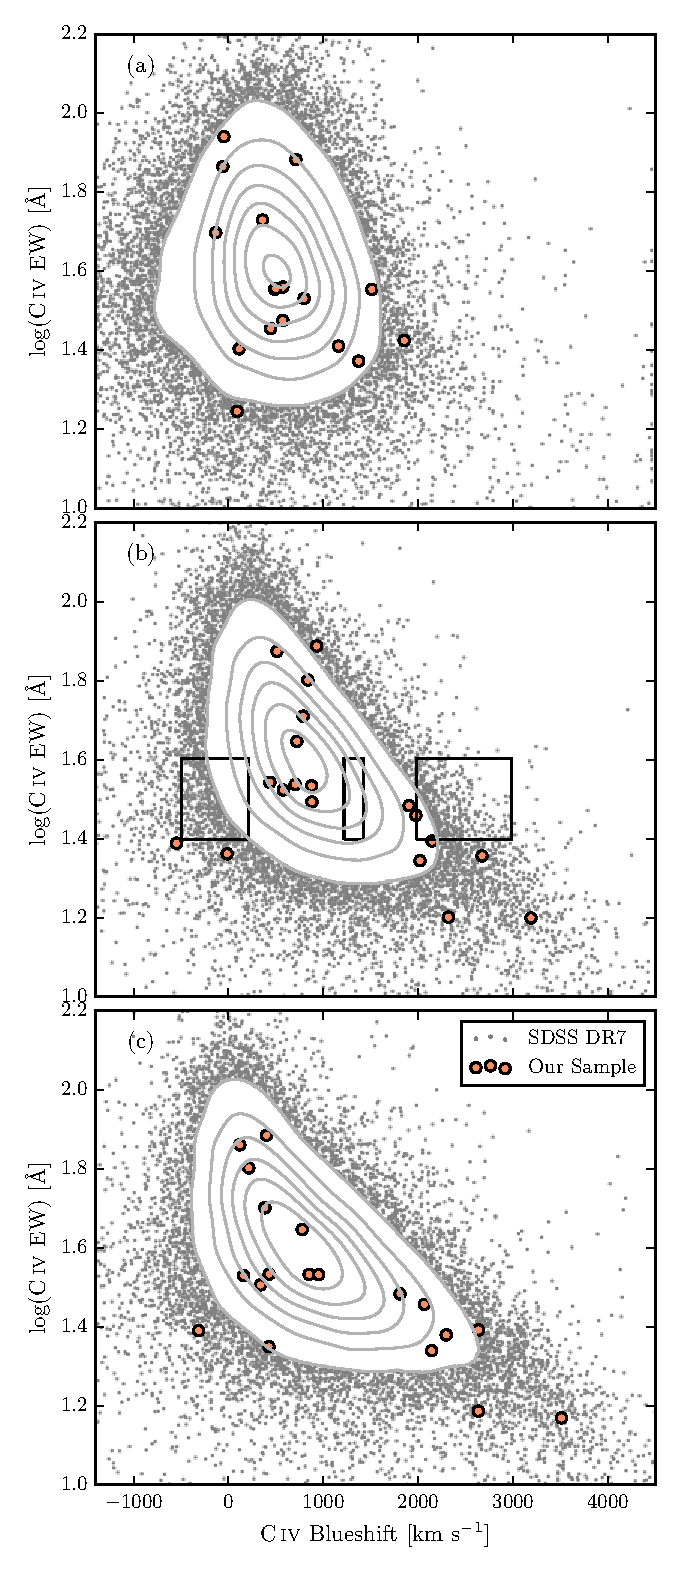
\includegraphics[width=\columnwidth]{figures/chapter02/civ_space.pdf}
    \caption{Rest-frame EW versus blueshift of the broad \ion{C}{IV}-emission line for 32,157 SDSS DR7 quasars at $1.6 < z < 3.0$ ({\it grey}) and our sample ({\it orange}). Panel (a) uses \ion{C}{IV} line parameters from \citet{shen11} and SDSS pipeline systemic redshifts. Panels (b) and (c) use systemic redshifts from \citet{hewett10} and Allen \& Hewett (2016, in preparation) respectively, and \ion{C}{IV} line measurements described in Sec.~\ref{sec:civmeasure}. In regions of high point-density, contours show equally-spaced lines of constant probability density generated using a Gaussian kernel-density estimator. The three rectangles in panel (b) show the regions of parameter space used to generate the composite spectra shown in Fig.~\ref{fig:civ_composites}. } 
    \label{fig:civ_space}
\end{figure}

Historically, the parametrisation of the \ion{C}{IV} emission-line properties for quasars in large surveys has not proved straightforward because the \ion{C}{IV} emission line has itself been used in the determination of the quasar redshifts. 
The SDSS provided the first catalogue of tens of thousands of redshift $z>$1.6 quasars with spectra of adequate velocity resolution and S/N that effective statistical studies of the rest-frame ultraviolet emission-line properties, including line-shape, have proved possible.

The comprehensive compilation of quasar properties for the SDSS DR7 quasars by \citet{shen11} provides a natural starting point for population studies. 
In Fig.~\ref{fig:civ_space}a we plot the \ion{C}{IV}-blueshift versus \ion{C}{IV}-emission equivalent width (EW) using the SDSS pipeline redshifts and the blueshifts calculated by \citet{shen11}. 
The grey points show all SDSS DR7 quasars for which measurements exist and the orange circles show the 19 quasars with near-infrared spectra presented in this paper.  
A strong trend in the blueshift values as a function of line EW is not evident in Fig.~\ref{fig:civ_space}; structure in the parameter space is being masked because the \ion{C}{IV} emission line is itself being used in the determination of the quasar redshifts. 

The redshift-determination scheme of \citet{hewett10} provided much improved redshifts, not least because the redshift estimates for the majority of quasars were derived using emission-lines other than the \ion{C}{IV}-line itself. 
Figure \ref{fig:civ_space}b shows SDSS DR7 quasars in the same \ion{C}{IV} parameter space as Figure \ref{fig:civ_space}a, but now using \citet{hewett10} redshifts. 
The improved redshift estimates are predominantly responsible for the differences seen in Fig.~\ref{fig:civ_space}a and b; the appearance in Fig.~\ref{fig:civ_space}b of the extension to high blueshift for quasars with low \ion{C}{IV} EW is particularly evident.

The large systematic variation in the \ion{C}{IV} emission-line profile within the population is evident from figures 11 and 12 of \citet{richards11}. 
The plots and analysis in \citet{richards11} employ the quasar redshifts from \citet{hewett10} but, as is evident from the figures, the systematic variation in the \ion{C}{IV} shape is correlated with changes in the quasar SEDs, including the strengths of the \ion{Si}{III}$\lambda$1892 and \ion{C}{III}$\lambda$1908 emission lines in the rest-frame ultraviolet. As a consequence, the redshifts from \citet{hewett10} still suffer from systematic errors that are correlated with the shape, and particularly the blueshift, of the \ion{C}{IV} emission line.
The nature of the systematic variations in the quasar ultraviolet SEDs are such that for quasars with close-to symmetric \ion{C}{IV} profiles and line centroids close to the systemic redshift, the \citet{hewett10} redshifts result in \ion{C}{IV} blueshifts that are overestimated by a few hundred \kms, whereas, for quasars with strong blue-asymmetric \ion{C}{IV} profiles and line centroids displaced significantly to the blue of the systemic redshift, the \ion{C}{IV} blueshifts are underestimated by, in the most extreme cases, up to 1200\kms. 

Figure~\ref{fig:civ_space}c shows the \ion{C}{IV} emission line parameters calculated using a new redshift-estimation algorithm (Allen \& Hewett 2016, in preparation) that takes account of the quasar SED variations, producing redshifts independent of the large systematic shape changes seen in the \ion{C}{IV} emission line. 
The low-ionization emission lines visible in the rest-frame ultraviolet (over wavelengths from \ion{Mg}{II}$\lambda\lambda$2796,2803 down to the \ion{O}{I}$\lambda$1304+\ion{Si}{II}$\lambda$1307 blend) using the new redshift-algorithm are located at rest-frame wavelengths in excellent agreement with the systemic redshift defined using the rest-frame narrow-line optical \ion{O}{III}$\lambda\lambda$4960,5008 and broad-line \hb and \hans.

The systematic trends seen in Fig.~\ref{fig:civ_space}b, in particular the extension to high blueshift at low \ion{C}{IV} EW, become more apparent in Fig.~\ref{fig:civ_space}c, as expected from consideration of the known SED-related errors in the redshifts from \citet{hewett10}.
A population of quasars with only modest blueshifts and low EW is also apparently still present. 

\subsection{\ion{C}{IV} emission line blueshift measurements}
\label{sec:civmeasure}

The differences in the distribution of \ion{C}{IV} emission line properties seen in the three panels of Fig.~\ref{fig:civ_space} are due primarily to the change in the systemic redshift estimates. 
It is also necessary, however, to obtain a measure of the \ion{C}{IV} emission line `location' in order to calculate the blueshifts. 
When working with moderately-sized samples, parametric fits to the emission-line profile may be undertaken using careful mask-definition to minimise the effect of absorption features on the profiles used for the parametrization, and this is the approach we follow below in Section~\ref{sec:line_measurements}. 
Effective analysis of the tens of thousands of spectra from SDSS DR7, and now DR12, however, requires a more robust scheme to determine a \ion{C}{IV}-blueshift estimate that is not very sensitive to the range of S/N among the spectra or the presence of narrow absorption systems within the \ion{C}{IV}-emission profile. 
\citet{shen11} provide a discussion (their section~3) of the factors that effect the measurement of broad emission lines in quasar spectra of modest S/N. 
Their careful analysis of the \ion{C}{IV} emission properties employed the results of parametric fits of three Gaussians to the spectra. 
Our own experiments in quantifying the \ion{C}{IV} emission properties of SDSS spectra showed that a simple non-parametric measure of the \ion{C}{IV} emission location reduced the number of outliers significantly. 
Visual inspection of spectra demonstrated that the improvement is due primarily to the identification of, and interpolation over, associated and outflow absorption systems, which forms part of the non-parametric measurement scheme. 

We therefore chose to use a non-parametric scheme to measure the blueshift of the \ion{C}{IV} line, which we will now describe. 
A continuum is first defined as a power-law of wavelength, $f(\lambda) \propto \lambda^{-\alpha}$, with the slope, $\alpha$, determined using the median\footnote{The median is used to improve the robustness of the continuum estimate from the relatively small wavelength intervals.} values of the flux in two continuum windows at 1445--1465 and 1700--1705\AA\, (the same wavelengths as adopted by \citet{shen11}). 
The \ion{C}{IV} emission line is taken to lie within the wavelength interval 1500-1600\AA, a recipe that is commonly adopted \citep[e.g.][]{shen11, denney13}. 
To reduce the impact of narrow absorption systems on the emission-line profile a `pseudo continuum' is defined by applying a 41-pixel median filter to the quasar spectrum.
Pixels within the \ion{C}{IV} profile that lie more than 2$\sigma$ below the pseudo-continuum are deemed to be affected by absorption and added to an `absorber'-mask. 
Two pixels on either side of each such pixel are also included in the mask. 
For each masked pixel, the flux values in the spectrum are replaced by values from the pseudo-continuum. 

The wavelength that bisects the cumulative total line flux, $\lambda_{half}$, is recorded and the blueshift (in \kms) defined as $c\times$(1549.48-$\lambda_{half}$)/1549.48 where $c$ is the velocity of light and 1549.48\AA \ is the rest-frame wavelength for the \ion{C}{IV} doublet\footnote{The adopted \ion{C}{IV} rest-frame wavelength assumes an optically thick BLR, in which case the contribution from each component is equal. Adopting a 2:1 ratio (appropriate for an optically thin BLR) changes the blueshifts by $\sim$80\kms.}. 
Positive blueshift values indicate an excess of emitting material moving towards the observer and hence out-flowing from the quasar.
\citet{hewett10} redshifts are used to define the quasar rest-frame. 

\subsection{Sample selection - \ion{C}{IV} properties}

The primary aim of the paper is to investigate the potential systematic effects on the \ion{C}{IV}-emission based BH masses for quasars with large, $\gtrsim$1200\kms, \ion{C}{IV} blueshifts, using the properties of the \ha emission line to provide BH-mass estimates for the objects unbiased by non-virial contributions to the emission-line profile.
The orange symbols in Fig.~\ref{fig:civ_space} show the \ion{C}{IV} parameters of our quasar targets for which near-infrared spectra of adequate S/N were obtained. 
These quasars were selected using our non-parametric blueshift measures (based on the \citet{hewett10} redshifts). 
The sample of 19 quasars spans the full dynamic range in \ion{C}{IV}-parameters based on the \citet{hewett10} systemic redshifts and the coverage is in fact even more complete when using the forthcoming SED-independent redshifts from Allen \& Hewett (2016, in preparation).
As is evident from the sparsity of quasars with large \ion{C}{IV} blueshifts when the SDSS pipeline systemic redshifts are used (Fig.~\ref{fig:civ_space}a), improvements in the estimation of systemic redshifts from ultraviolet spectra have been a crucial factor in allowing us to reliably select a sample of quasars with a range of \ion{C}{IV} blueshifts. 
In subsequent sections we re-derive the systemic redshifts and \ion{C}{IV} blueshifts for this sample using parametric fits to the \ha and \ion{C}{IV} emission (the former from our-near infrared observations). 
Thus, while the systematic trends in BH masses inferred from measurements of the \ion{C}{IV} emission line depend on the distribution of \ion{C}{IV} emission line properties within the quasar population, the results of our analysis of the \ha and \ion{C}{IV} emission line properties are independent of the redshifts used to produce the panels in Fig.~\ref{fig:civ_space}.  

\subsection{Relation to virial BH mass estimates}
\label{sec:blueshiftmasses}

\begin{figure}
    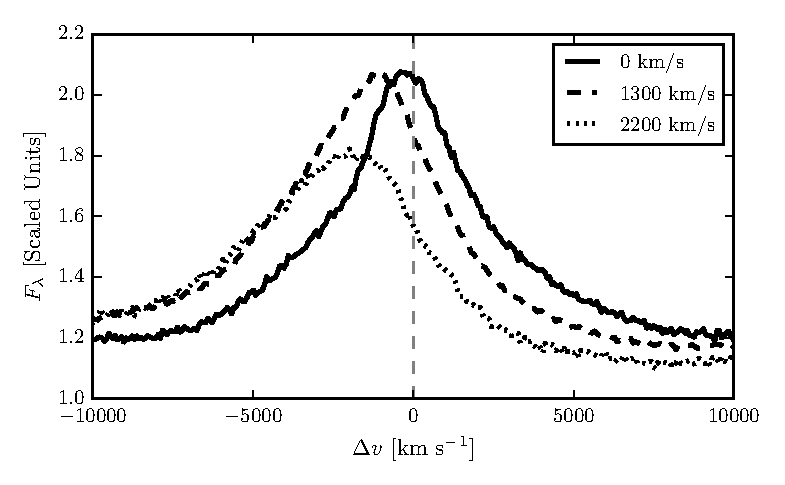
\includegraphics[width=\columnwidth]{figures/chapter02/civ_composites.pdf}
    \caption{Composite spectra of the \ion{C}{IV}-emission line as a function of \ion{C}{IV} blueshift for SDSS DR7 quasars. The quasars contributing to each composite are indicated in Fig.~\ref{fig:civ_space}b. Virtually the entire \ion{C}{IV}-profile appears to shift blueward and the change in line shape is not simply an enhancement of flux in the blue wing of a still identifiable symmetric component. In order of increasing \ion{C}{IV} blueshift, the composite spectra have FWHM 4870, 5610, and 6770 \kms\, and EW 33.1, 31.6, and 28.8 \AA.}
    \label{fig:civ_composites}
\end{figure}

In general, researchers studying quasar demographics at high-redshift adopt estimates of BH masses based on the width of \ion{C}{IV}-emission, without reference to the blueshift of the \ion{C}{IV}-emission \citep[e.g.][]{vestergaard04,kollmeier06,gavignaud08,vestergaard08,vestergaard09,kelly10,kelly13}.  
The systemic redshift is often assumed to be given by the peak of the \ion{C}{IV} emission, regardless of whether there is evidence that the line is shifted or not.
Figure~\ref{fig:civ_composites} shows the shape of the \ion{C}{IV}-emission in composite spectra constructed from SDSS DR7 quasars with EW(\ion{C}{IV})=25-40\AA, as a function of \ion{C}{IV} blueshift. 
Quasars classified as BALs, or possessing strong associated absorbers have been excluded, and the composite-spectra shown are derived using an arithmetic mean of a minimum of 200 spectra at each blueshift. 
The blueshifts and EWs of the quasars contributing to each of the composites are indicated by the boxes in Fig.~\ref{fig:civ_space}b.  
The profiles show how, at large values of blueshift ($\gtrsim$2000\kms) the \ion{C}{IV}-profile is displaced to the blue by amounts comparable to the FWHM of the profile.

A possible origin of the blueshifts is the presence of a disc-wind \citep[see][for recent papers]{gallagher15, higginbottom15} but, irrespective of the physical origin of the high-blueshift \ion{C}{IV}-profiles, measures of the emission-line `width' do not relate simply to virialized motions of the emitting gas under the gravitational influence of the BH. 
On the other hand, \citet{denney13} point out that any radiatively driven wind will have a velocity comparable to the escape velocity, i.e. approximately twice the virial velocity.
Even if dominated by an outflow component, the \ion{C}{IV} line width might therefore still be expected to relate to the BH mass. 


\section{Observations}
\label{sec:observations}

\begin{table*}
  \centering
  \vspace*{-0.4cm}
  \caption{Summary of near-infrared spectroscopic observations with LIRIS.}
  \label{tab:obsproperties}
  \vspace*{-0.1cm}
  \begin{minipage}{16cm}
    \begin{tabular}{ccccccccc} 
    \hline
    SDSS Name & SDSS DR & $z$\footnote{From \citet{hewett10}.} & $i_{\rm SDSS}$ & UTC Date & T$_{\rm exp}$ (s) & S/N(\ion{C}{IV})\footnote{\label{footnote-label}Measured in the continuum and quoted per resolution element.} & S/N(\hbns)\textsuperscript{\small \ref{footnote-label}} & S/N(\hans)\textsuperscript{\small \ref{footnote-label}} \\
    \hline
    073813.19+271038.1 & DR12 & 2.4508 & 18.80 & 2015-04-01 & 720 & 29.13 & 17.27 & 10.0 \\
    074352.61+245743.6 & DR12 & 2.1659 & 19.09 & 2015-04-04 & 2160 & 8.64 & 18.68 & 11.43 \\
    080651.54+245526.3 & DR12 & 2.1594 & 18.91 & 2015-04-01 & 1200 & 10.37 & 6.04 & 3.91 \\
	085437.59+031734.8 & DR7 & 2.2504 & 18.41 & 2015-03-31 & 2520 & 26.58 & 5.82 & 3.09 \\
	085856.00+015219.4 & DR12 & 2.1675 & 17.62 & 2015-04-04 & 1800 & 66.16 & 24.37 & 12.71 \\
	110454.73+095714.8 & DR12 & 2.4238 & 19.12 & 2015-04-03 & 1440 & 19.41 & 10.75 & 7.81 \\
	123611.21+112921.6 & DR12 & 2.1527 & 18.53 & 2015-04-04 & 1680 & 35.24 & 21.3 & 11.51 \\
	124602.04+042658.4 & DR12 & 2.4473 & 18.49 & 2015-04-01 & 960 & 35.34 & 8.1 & 5.73 \\
	130618.60+151017.9 & DR12 & 2.4020 & 19.00 & 2015-04-05 & 840 & 29.83 & 8.91 & 5.13 \\
	131749.78+080616.2 & DR12 & 2.3791 & 19.04 & 2015-04-05 & 2880 & 19.25 & 5.6 & 3.32 \\
	132948.73+324124.4 & DR12 & 2.1684 & 18.40 & 2015-04-01 & 2520 & 32.58 & 10.4 & 6.96 \\
	133646.87+144334.2 & DR7 & 2.1422 & 18.84 & 2015-04-01 & 1200 & 15.2 & 23.82 & 16.34 \\
	133916.88+151507.6 & DR12 & 2.3157 & 18.52 & 2015-04-03 & 2880 & 20.52 & 5.79 & 3.28 \\
	140047.45+120504.6 & DR12 & 2.1722 & 18.29 & 2015-04-02 & 840 & 36.64 & 9.83 & 5.68 \\
	152529.17+292813.2 & DR12 & 2.3605 & 17.52 & 2015-04-04 & 1440 & 80.55 & 2.17 & 1.5 \\
	153027.37+062330.8 & DR12 & 2.2198 & 18.62 & 2015-04-04 & 1800 & 29.9 & 21.01 & 12.58 \\
	153848.64+023341.1 & DR12 & 2.2419 & 17.56 & 2015-04-01 & 2520 & 64.82 & 5.63 & 3.56 \\
	161842.44+234131.7 & DR7 & 2.2824 & 18.49 & 2015-04-04 & 1320 & 23.37 & 11.1 & 6.43 \\
	163456.15+301437.8 & DR12 & 2.4901 & 18.29 & 2015-04-01 & 1920 & 36.06 & 9.44 & 8.63 \\
    \hline
    \end{tabular}
  \vspace*{-0.4cm}
  \end{minipage}
\end{table*}

Near-infrared spectra were obtained with the Long-slit Intermediate Resolution Infrared Spectrograph (LIRIS) mounted on the 4.2m William Herschel Telescope (WHT) at the Observatorio del Roque de los Muchachos (La Palma, Spain). 
Observations took place over four non-contiguous nights from 2015 March 31 to April 4. 
Approximately one night was lost due to poor weather and a further half-night was affected by poor transparency due to cloud. 
A one arcsecond slit-width was employed and the LIRIS $H+K$ low-resolution grism was selected, which covers the spectral ranges 1.53--1.79\,$\mu$m and 2.07--2.44\,$\mu$m with a dispersion of 9.7\AA/pixel. 
The spatial scale of the instrument is 0.25 arcsec/pixel. 
Observations were divided into 60\,s sub-exposures and performed in an ABBA nodding pattern, with the object placed at two positions along the slit 12 arcsec apart. 
Bright A0-5V stars were observed at similar air-masses to the targets in order to provide both telluric absorption corrections and a flux calibration of the quasar spectra.

The raw LIRIS data frames incorporate a known `pixel shift' which was first removed from all frames using the LIRIS data reduction package {\tt LIRISDR}. 
Subsequent data reduction was undertaken with standard {\tt IRAF}\footnote{IRAF is distributed by the National Optical Astronomy Observatory, which is operated by the Association of Universities for Research in Astronomy (AURA) under a cooperative agreement with the National Science Foundation.} procedures.  
The flat-field images, which were taken at the beginning of each night via illumination of the dome, were averaged and normalised to remove any wavelength-dependent signature. 
Each individual two-dimensional spectrum was then flat-field corrected. 
Consecutive AB and BA pairs of two-dimensional spectra were subtracted to remove the sky background. 
All the subtracted AB/BA-pairs for a target were then averaged to give the final two-dimensional spectrum.

The size of the one-dimensional spectrum extraction windows, in the slit direction, varied from 6-10 pixels. 
To increase the S/N, optimal variance-weighted extraction with sigma clipping was employed. 
For the fainter objects in our sample we were unable to trace the spectrum across the dispersion axis reliably and the trace from a telluric standard-star observation, observed at a similar air mass and time, was used instead. 
The wavelength calibration, using argon and xenon lamp exposures, resulted in root mean square errors in the range 1.01--1.71\,\AA, with a mean of 1.47\AA. 
The telluric standard star observations were reduced using the same steps described above. 
The stellar continuum was divided out of the standard star spectrum, which was then divided into the quasar spectrum to remove telluric absorption features. 
The spectral type and magnitude of the standard star were used to flux calibrate the quasar spectrum both in a relative and absolute sense.
Variable atmospheric conditions combined with the narrow slit width resulted in a significant level of uncertainty in the absolute flux calibration for the quasar observations. 
The use of the UKIDSS broadband magnitudes ($H$ and $K$) to normalise the spectra results in a significantly improved calibration. 

\begin{figure}
    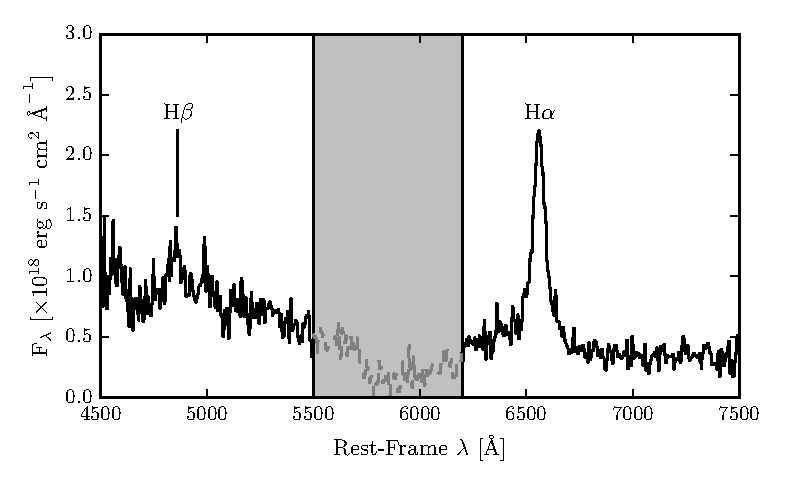
\includegraphics[width=\columnwidth]{figures/chapter02/example_spectrum.pdf} 
    \caption{LIRIS spectrum of SDSSJ1246+0426. The gap between the $H$ and $K$ bands ($\sim$5500-6300\,\AA) has been greyed-out.}
    \label{fig:example_spectrum}
\end{figure}

Spectra with sufficient S/N for analysis of the \ha emission line properties were obtained for a total of 19 quasars. 
Sixteen of the 19 quasars have been re-observed in the Sloan Digital Sky Survey-III: Baryon Oscillation Spectroscopic Survey \citep[SDSS-III/BOSS;][]{dawson13} and the spectra are available in the SDSS DR12 quasar catalogue \citep{paris17}. 
As the BOSS-spectra have higher S/N compared to those in DR7, we have used the BOSS spectra when available.
A typical reduced LIRIS spectrum is shown in Fig.~\ref{fig:example_spectrum}. 
A log of the observations, the quasar positions, magnitudes and redshifts, along with the S/N achieved for the \hbns, \ha and \ion{C}{IV} emission line regions (the last from the optical SDSS/BOSS spectra) are listed in Table~\ref{tab:obsproperties}.
The S/N, which is given per resolution element, was measured in the continuum in the region around the emission lines. 
The full SDSS name is given in Table~\ref{tab:obsproperties}; in the subsequent tables and text we will refer to objects using an abbreviated name of the form SDSSJHHMM+DDMM.

Although the S/N is similar in the continuum regions adjacent to the \ha and \hb emission lines, in practice the much lower EW of \hb compared to \ha meant that both parametric and non-parametric characterisation of the emission-line parameters did not produce results that could be used in this investigation. 
The individual \hb profiles were thus not employed, although a composite spectrum of the \hb region is used below.

\section{Emission line measurements} % (fold)
\label{sec:line_measurements}

Virial BH mass estimators are calibrated using either the FWHM or dispersion ($\sigma$; derived from the second-moment velocity) of a broad emission line \citep[e.g.][]{vestergaard06,park13}. 
Complications which are encountered when measuring line widths include how to model the `continuum' flux, where to define the limits of the line emission, and how to deal with absorption. 
All of these issues are exacerbated when working with low S/N data \citep[see][for a discussion]{denney13}. 
In Section~\ref{sec:civmeasure} we measured the blueshift of \ion{C}{IV} for tens of thousands of SDSS DR7 quasar spectra. 
This allowed us to quantify the distribution of \ion{C}{IV} blueshift values and hence select a subset for near-infrared observations which have \ion{C}{IV} blueshifts spanning the full range of this distribution (Fig.~\ref{fig:civ_space}).
A non-parametric scheme was employed because, in comparison to recipes involving the fitting of multiple Gaussian (or other parametric) profiles, it was found to be more robust and less sensitive to the range of S/N among the spectra and to the presence of narrow absorption systems within the \ion{C}{IV}-emission profile.
In this section we will use a different approach, and measure the line properties by fitting a parametric model to the data. 
When working with a small number of spectra, it is possible to use careful mask-definition to minimise the effect of absorption features on the profiles used for the parametrization.
The purpose of the model fits is purely to best represent the intrinsic line profile, and no physical meaning is attached to the individual model components. 
We will now describe the parametric model and fitting procedure used for each emission line. 
The models were fit using a standard variance-weighted least squares minimisation procedure employing the Levenberg-Marquardt algorithm. 
Prior to the fit, the spectra were visually inspected and regions significantly affected by absorption were masked and excluded.

\begin{table*}
  \centering
  \caption{Summary of the fitting regions and the parameters of the models used to fit the \ion{C}{IV} and \ha emission lines.}
  \label{tab:fittingproperties}
    \begin{tabular}{ccccccccc}
    \hline
    & \multicolumn{2}{c}{Fitting Region [\kms]} & \multicolumn{2}{c}{Continuum Region[\AA]} & GH Order & Gaussians & \multicolumn{2}{c}{$\chi^2_{\nu}$} \\
    Name & \ion{C}{IV}  & \hans & \ion{C}{IV} & \hans & \ion{C}{IV} & \hans & \ion{C}{IV} & \hans \\
    \hline
    0738+2710 & -9570,9770 & -7530,10740 & 1445-1465,~~1700-1705 & 6000-6250,~~6800-7000 & 6 & 2 & 0.66 & 1.0 \\
    0743+2457 & -9570,9770 & -7530,10740 & 1445-1465,~~1700-1705 & 6004-6210,~~6800-7000 & 2 & 2 & 0.84 & 1.0 \\
    0806+2455 & -9570,9770 & -9219,10759 & 1445-1465,~~1700-1705 & 6000-6250,~~6800-7000 & 3 & 1 & 0.87 & 0.83 \\
    0854+0317 & -9570,9770 & -7530,10740 & 1445-1465,~~1700-1705 & 5989-6135,~~6800-7000 & 3 & 2 & 0.91 & 0.85 \\
    0858+0152 & -20000,7400 & -7530,10740 & 1423-1428,~~1700-1705 & 6000-6200,~~6800-7000 & 2 & 2 & 0.94 & 0.96 \\
    1104+0957 & -9570,9770 & -7530,10740 & 1445-1465,~~1700-1705 & 6000-6250,~~6801-6845 & 6 & 2 & 0.68 & 0.95 \\
    1236+1129 & -15363,7650 & -8904,10590 & 1445-1465,~~1700-1705 & 6063-6210,~~6800-7000 & 3 & 2 & 0.84 & 0.89 \\
    1246+0426 & -9570,9770 & -7530,10740 & 1445-1465,~~1700-1705 & 6000-6250,~~6799-6906 & 4 & 2 & 0.66 & 0.83 \\
    1306+1510 & -13000,7800 & -7530,10740 & 1445-1465,~~1700-1705 & 6000-6250,~~6800-7000 & 2 & 3 & 0.73 & 0.18 \\
    1317+0806 & -9198,9755 & -7530,10740 & 1445-1465,~~1700-1705 & 6000-6250,~~6800-7000 & 2 & 1 & 0.78 & 2.16 \\
    1329+3241 & -12000,9000 & -7605,7406 & 1445-1461,~~1700-1705 & 6000-6250,~~6800-7000 & 3 & 2 & 0.61 & 0.84 \\
    1336+1443 & -14000,10000 & -10131,10674 & 1445-1465,~~1700-1705 & 6000-6250,~~6800-7000 & 3 & 2 & 0.87 & 1.51 \\
    1339+1515 & -12000,11000 & -7530,10740 & 1445-1465,~~1700-1705 & 6046-6250,~~6800-7000 & 4 & 1 & 0.69 & 0.14 \\
    1400+1205 & -15000,10000 & -2000,10815 & 1445-1465,~~1700-1705 & 6000-6250,~~6800-7000 & 6 & 2 & 0.82 & 0.2 \\
    1525+2928 & -9570,9770 & -7586,8080 & 1459-1466,~~1700-1705 & 6055-6251,~~6800-7000 & 4 & 1 & 0.49 & 0.39 \\
    1530+0623 & -12000,10000 & -7530,10740 & 1445-1465,~~1700-1705 & 6127-6186,~~6800-7000 & 4 & 3 & 0.84 & 1.14 \\
    1538+0233 & -13500,9000 & -7530,10740 & 1450-1465,~~1700-1705 & 6000-6250,~~6855-7002 & 4 & 2 & 0.61 & 0.82 \\
    1618+2341 & -9190,9770 & -7530,10740 & 1445-1465,~~1689-1697 & 6000-6250,~~6800-7000 & 4 & 2 & 1.16 & 0.93 \\
    1634+3014 & -9570,9770 & -8400,8500 & 1445-1465,~~1700-1705 & 6000-6250,~~6736-6779 & 3 & 2 & 0.59 & 0.22 \\
    \hline
  \end{tabular}
\end{table*}

\subsection{\ion{C}{IV}}

We first measure and subtract the local continuum emission, by fitting a power-law to two windows on either side of the line emission, as described in Section~\ref{sec:civmeasure}. 
For a small number of objects, absorption features, or artefacts, in the spectrum necessitated modest adjustments to the window extents, which are specified in Table~\ref{tab:fittingproperties}. 
The continuum-subtracted spectra are then transformed from wavelength units into units of velocity relative to the rest-frame line-transition wavelength for the \ion{C}{IV} doublet (1549.48\AA, assuming equal contributions from both components). 
The parametric model is ordinarily fit within the same 1500--1600\,\AA \, window used in Section~\ref{sec:civmeasure}, which corresponds to approximately $\pm 10\,000$ \kms\, from the rest-frame transition wavelength. 
The line-window was extended if significant flux in the profile was present blueward of the short wavelength limit. 
The adopted line-fitting windows, in units of velocity from the rest-frame transition wavelength, are given in Table~\ref{tab:fittingproperties}. 

To fit the \ion{C}{IV} profile we employed Gauss-Hermite (GH) polynomials, using the normalisation of \citet{marel93} and the functional forms of \citet{cappellari02}.
We allowed up to six components in the GH polynomial model, but in many cases a lower order was sufficient; the polynomial order used for each line is given in Table~\ref{tab:fittingproperties}.
It is also a common practice to fit the \ion{C}{IV} emission profile with two or three Gaussian components \citep[e.g.][]{shen11}. 
We opted to use a GH-polynomial model primarily because it provided a significantly better fit to the most blueshifted and asymmetric \ion{C}{IV} line (in SDSSJ0858+0152).  
Figure~\ref{fig:fitting_comparison} shows how a model with three Gaussian components underestimates the flux in the blue wing and overestimates the flux in the red wing of the line profile. 
Using the Gaussian model rather than the GH polynomial changes the FWHM, line dispersion, and blueshift by -3, -3, and 10\,per cent respectively.
We have highlighted SDSSJ0858+0152 because, of all the objects in our sample, the choice of model leads to the largest change in \ion{C}{IV} line parameters.
Even in this case, however, the differences are modest. 

\begin{figure}
    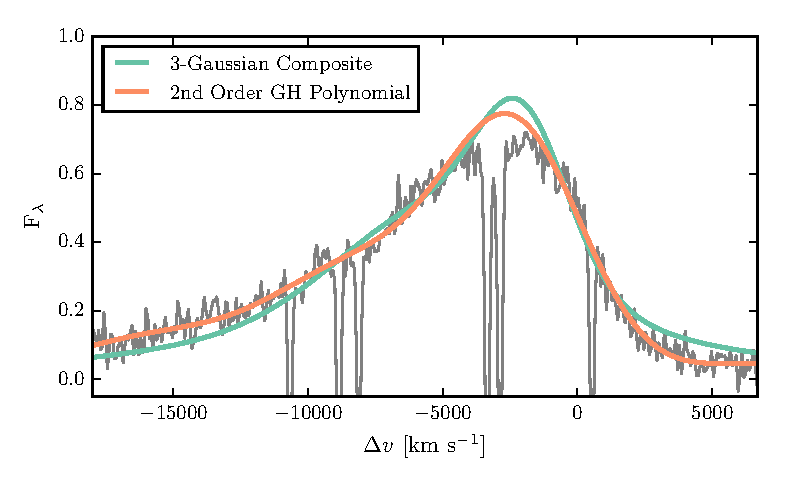
\includegraphics[width=\columnwidth]{figures/chapter02/fitting_comparison.pdf} 
    \caption{2nd-order Gauss-Hermite (GH) polynomial and 3-component Gaussian fit to the \ion{C}{IV}-emission line of SDSSJ0858+0152, which is the most blueshifted in our sample. We derive line parameters from the GH polynomial fit; using the Gaussian model changes the FWHM, line dispersion, and blueshift by -250, -150, and 500 \kms respectively. For the \ion{C}{IV} lines of all other quasars in our sample the GH polynomial and Gaussian models provide equally good fits.} 
    \label{fig:fitting_comparison}
\end{figure}

For every other \ion{C}{IV} line in our sample we found only marginal differences in our best-fit line parameters when, rather than using a GH polynomial model, the \ion{C}{IV} emission was fit using a composite model of up to three Gaussians. 
Our best-fit parameters are also in good agreement with \citet{shen11}, who employ a multi-Gaussian parametrization\footnote{The \citet{shen11} parameters are derived from the SDSS DR7 spectra, whereas 16 out of 19 of our fits are to higher S/N BOSS DR12 spectra.}.  
The scatter between the \citet{shen11} results and our own is 0.1\,dex about the one-to-one relation and, as expected, is larger for lines with smaller EWs. 

\subsection{\ha}

We employ the same continuum subtraction and fitting method as for \ion{C}{IV}, with the continuum and fitting windows as given in Table~\ref{tab:fittingproperties}. 
We adopt a rest-frame transition wavelength of 6564.89\,\AA\, to transform wavelengths into equivalent Doppler velocities. 
We used a simple model with up to three broad Gaussian components to fit the \ha emission line.
We opted against parametrizing the \ha line using a GH polynomial because the extra degrees of freedom in this model did not improve the quality of the fits\footnote{The emission line parameters and subsequent analysis do not depend on whether line parameters from multiple-Gaussian or GH-polynomial model fits are used.}.
Upon inspection of the residuals from the fit, we also found no evidence that additional model components for narrow \hans, \ion{N}{II}\ll6548,6584 and \ion{S}{II}\ll6717,6731 were required.
Furthermore, narrow \ion{O}{III}\ll4960,5008 emission is relatively weak in these spectra.

The sole exception is the \ha line in the spectrum of SDSSJ0738+2710.
In addition to having the narrowest \ha line, this spectra also has the strongest narrow \ion{O}{III} component (EW = 63\,\AA), which suggests that a contribution from the narrow-line region might be important.  
Introducing a single Gaussian for the narrow emission, while retaining a double Gaussian for the broad emission, the FWHM of the broad component increases to 3400\,\kms (compared to 1580\,\kms without the narrow component). 
For consistency, the parameters quoted in Table~\ref{tab:emissionproperties} are from the model with no narrow component. 
However, because the properties derived from the emission line width (the BH mass and the mass-normalised accretion rate) are strongly biased by the probable contribution from the narrow-line region, SDSSJ0738+2710 is excluded from the analysis in Section~\ref{sec:results}. 

\subsection{Comparison of H$\alpha$ and H$\beta$ profiles}

Virial BH mass estimators are typically based on the width of \hbns. 
However, the \ha and \hb emission is believed to originate from the same gas and the transformation between the emission-line velocity widths is expected to be well defined. 
\citet{greene05}, using a sample of 162 quasars with high S/N SDSS spectra, established the following relation between the \ha and \hb FWHM:

\begin{equation}
  \label{eq:hb2hawidth}
  \rm{FWHM}(\rm{H}\beta) = (1.07 \pm 0.07) \times 10^3 \left( \frac{ \rm{FWHM}(\rm{H}\alpha) }{10^3 ~\rm{km}~\rm{s}^{-1} } \right)^{(1.03 \pm 0.03)}
\end{equation}

\citet{greene05} found the root-mean-square scatter about this relation to be $\sim$ 0.1 dex. 
We do not have a sufficient number of robust \hb line measurements to test this relation directly.
However, we are in the process of acquiring a much larger sample of quasars with near-infrared spectra covering \ha and \hb at similar redshifts and luminosities to the sample presented here. 
The \ha and \hb line widths of this sample are in excellent agreement with the \citet{greene05} relation. 
To indirectly test the \hans/\hb line width relation for the sample presented here, we first constructed mean composite spectra in the \ha and \hb emission line regions to increase the S/N. 
The individual rest-frame spectra (defined using the wavelength of the \ha centroid) were interpolated on to a common wavelength grid. 
The spectra were then normalised using the continuum flux under the line centre, which was found by linearly interpolating between two emission-line free windows on either side of the line. 
Figure.~\ref{fig:balmer_composite} shows the composite \ha and \hb line regions overlaid and, as expected, the line profiles are closely matched.

\begin{figure}
    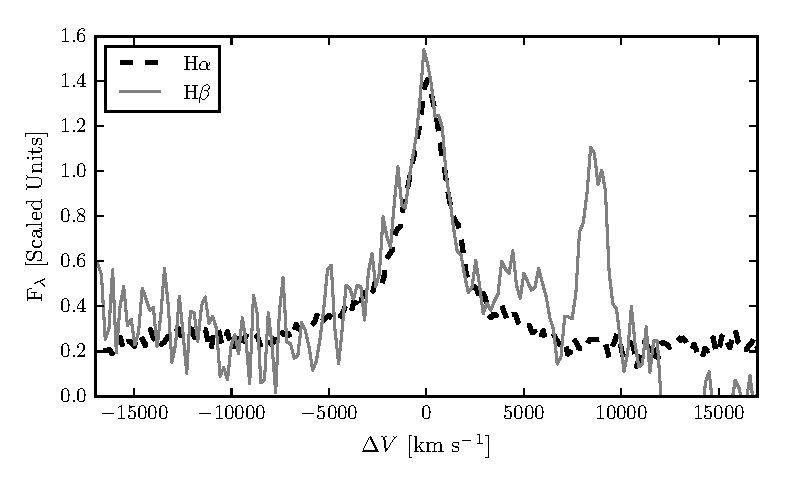
\includegraphics[width=\columnwidth]{figures/chapter02/ha_hb_composite.pdf} 
    \caption{The \ha and \hb emission line regions in the median composite spectrum, shown as function of the velocity shift from the respective predicted line peak wavelengths. The line fluxes have been scaled in order for the profile shapes to be readily compared. The \ha and \hb line profiles are very similar, which suggests a tight correlation between the \ha and \hb line widths. Quasar narrow-line emission from \ion{O}{III}\l5008.2 is visible but, overall, the \ion{O}{III}\ll4960,5008 emission is relatively weak in these spectra.}
    \label{fig:balmer_composite}
\end{figure}

\subsection{Emission line parameters}

\begin{table*}
  \centering
  \caption{Summary of emission line properties derived from parametric model fits to \ha and \ion{C}{IV}. }
  \label{tab:emissionproperties}
  \begin{tabular}{ccccccccc}
  \hline
  & & Blueshift & \multicolumn{2}{c}{FWHM} & \multicolumn{2}{c}{$\sigma$} & \multicolumn{2}{c}{EW}  \\
  & & [\kms] & \multicolumn{2}{c}{[\kms]} & \multicolumn{2}{c}{[\kms]} & \multicolumn{2}{c}{[\AA]} \\
  Name & $z$ (\hans) & \ion{C}{IV} & \ion{C}{IV} & \hans & \ion{C}{IV} & \hans & \ion{C}{IV} & \hans \\
  \hline
  0738+2710 & 2.4396 & $50\pm21$ & $2255\pm42$ & $1503\pm95$ & $2916\pm42$ & $1789\pm95$ & $54\pm2$ & $532\pm43$ \\
  0743+2457 & 2.1662 & $692\pm210$ & $5924\pm536$ & $6036\pm511$ & $3801\pm536$ & $3904\pm511$ & $33\pm4$ & $351\pm23$ \\
  0806+2455 & 2.1542 & $389\pm115$ & $3435\pm267$ & $4059\pm403$ & $3387\pm267$ & $1724\pm403$ & $51\pm4$ & $488\pm56$ \\
  0854+0317 & 2.2475 & $-403\pm134$ & $3940\pm354$ & $4436\pm522$ & $3448\pm354$ & $3146\pm522$ & $24\pm2$ & $617\pm90$ \\
  0858+0152 & 2.1692 & $4354\pm82$ & $8412\pm384$ & $3155\pm80$ & $5298\pm384$ & $3758\pm80$ & $28\pm1$ & $622\pm23$ \\
  1104+0957 & 2.4217 & $-299\pm55$ & $3590\pm112$ & $3307\pm334$ & $3259\pm112$ & $2723\pm334$ & $70\pm3$ & $441\pm72$ \\
  1236+1129 & 2.1559 & $2828\pm99$ & $7540\pm271$ & $3152\pm131$ & $4168\pm271$ & $3277\pm131$ & $28\pm1$ & $631\pm29$ \\
  1246+0426 & 2.4393 & $325\pm145$ & $4126\pm88$ & $4268\pm472$ & $3901\pm88$ & $2543\pm472$ & $48\pm1$ & $536\pm77$ \\
  1306+1510 & 2.3989 & $2043\pm84$ & $6660\pm158$ & $2626\pm330$ & $3905\pm158$ & $2145\pm330$ & $36\pm1$ & $349\pm52$ \\
  1317+0806 & 2.3748 & $437\pm289$ & $5256\pm182$ & $7188\pm946$ & $3675\pm182$ & $3033\pm946$ & $33\pm2$ & $374\pm67$ \\
  1329+3241 & 2.1637 & $652\pm113$ & $4528\pm491$ & $4908\pm410$ & $3819\pm491$ & $3350\pm410$ & $35\pm2$ & $428\pm35$ \\
  1336+1443 & 2.1466 & $3668\pm345$ & $8780\pm1003$ & $2954\pm67$ & $3772\pm1003$ & $3227\pm67$ & $20\pm2$ & $523\pm17$ \\
  1339+1515 & 2.3207 & $133\pm184$ & $3865\pm935$ & $8816\pm1072$ & $4501\pm935$ & $3627\pm1072$ & $44\pm2$ & $500\pm98$ \\
  1400+1205 & 2.1672 & $2492\pm107$ & $7590\pm290$ & $3231\pm227$ & $4363\pm290$ & $3103\pm227$ & $25\pm1$ & $642\pm55$ \\
  1525+2928 & 2.3572 & $612\pm536$ & $5697\pm128$ & $6360\pm1915$ & $4303\pm128$ & $2696\pm1915$ & $41\pm1$ & $458\pm186$ \\
  1530+0623 & 2.2169 & $1471\pm108$ & $5397\pm302$ & $3073\pm145$ & $4092\pm302$ & $2664\pm145$ & $26\pm1$ & $499\pm28$ \\
  1538+0233 & 2.2420 & $2018\pm80$ & $5567\pm100$ & $2892\pm253$ & $3596\pm100$ & $2415\pm253$ & $25\pm1$ & $465\pm75$ \\
  1618+2341 & 2.2755 & $42\pm53$ & $2516\pm161$ & $2669\pm175$ & $3312\pm161$ & $2359\pm175$ & $34\pm2$ & $425\pm39$ \\
  1634+3014 & 2.5018 & $1509\pm223$ & $6835\pm745$ & $6210\pm900$ & $4566\pm745$ & $3236\pm900$ & $26\pm1$ & $327\pm65$ \\
  \hline
  \end{tabular}
\end{table*}

\begin{figure*}
	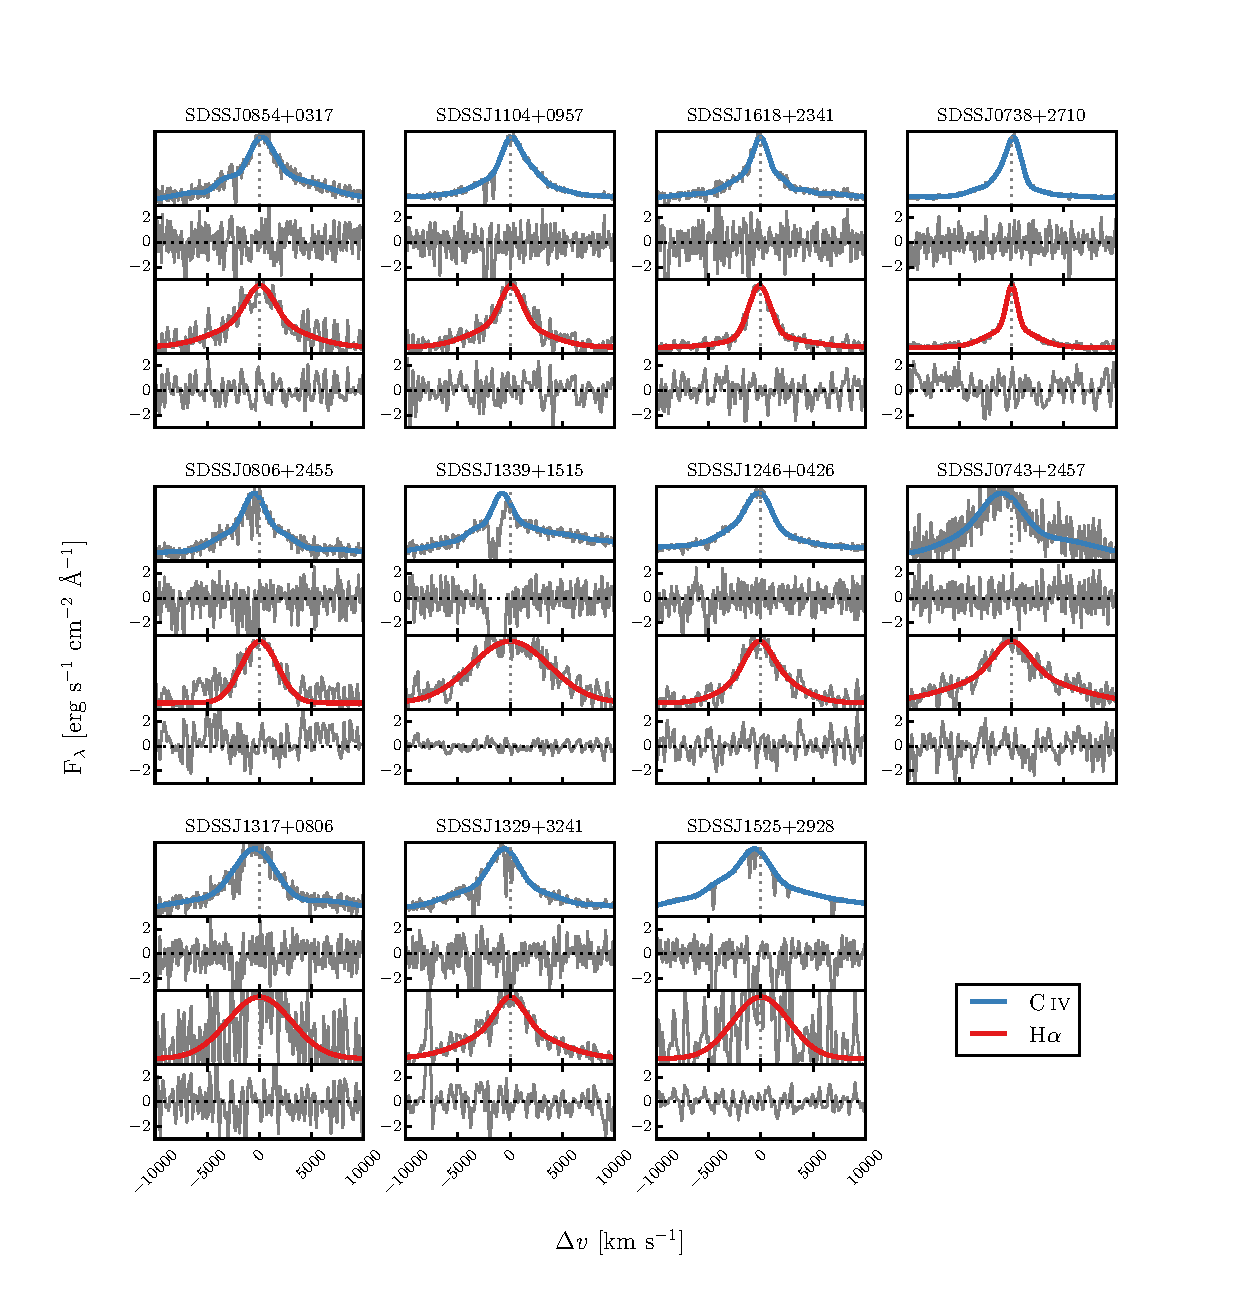
\includegraphics[width=2\columnwidth]{figures/chapter02/gridspectra_1.pdf} % ComparePeaksAll() in reduction_v12.py
    \caption{\ion{C}{IV} (SDSS/BOSS) and \ha (LIRIS) emission lines and best-fitting model. $\Delta{v}$ is the velocity shift from the line rest-frame transition wavelength, with the systemic redshift defined using the centroid of the fit to \hans. Objects are presented in order of increasing \ion{C}{IV} blueshift relative to the \ha centroid. Below each fit we plot the data-model residuals, scaled by the errors on the fluxes. }
    \label{fig:gridspectra_1}
\end{figure*}

\renewcommand{\thefigure}{\arabic{figure}}
\addtocounter{figure}{-1}
\begin{figure*}
	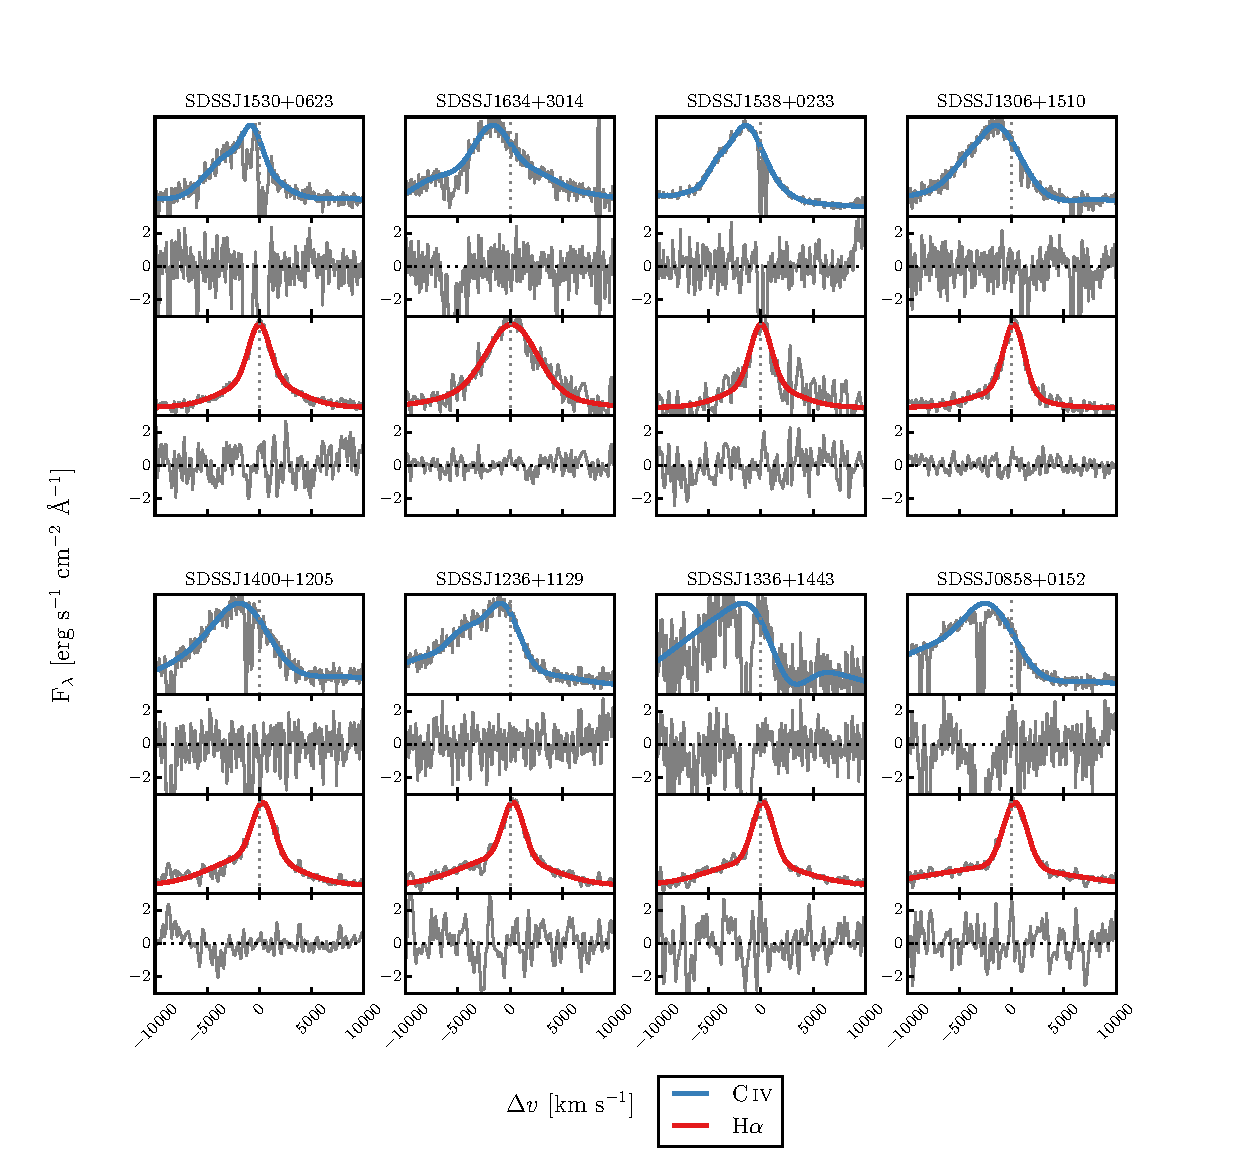
\includegraphics[width=2\columnwidth]{figures/chapter02/gridspectra_2.pdf}
    \caption{\it Continued}
    \label{fig:gridspectra_2}
\end{figure*}
\renewcommand{\thefigure}{\arabic{figure}}

In Fig.~\ref{fig:gridspectra_1} we show our best-fitting models overlaid on the observed flux in the spectral regions around \ion{C}{IV} and \hans. 
The spectra are presented in order of increasing \ion{C}{IV} blueshift. 
The Doppler velocities have been shifted so that the \ha emission line centroid is at 0\,\kms. 
The $y$-axes of the data-minus-model residual plots have deliberately been scaled by the spectrum flux errors.
The model fits are generally very good with only minimal systematic residuals. 
The only significant features seen in the residual \ion{C}{IV} spectra correspond to the location of narrow absorption lines which were excluded in the fitting procedure.
The continuum windows for a number of the \ha lines extend close to the edges of the $K$-band and uncertainties in the flux calibration, and hence continuum level, are almost certainly responsible for the low-amplitude, large-scale, systematic residuals seen in a number of objects (e.g. SDSSJ 0806+3455, 0858+0152, 1400+1205, 1538+0233). 
The amplitudes are, however, small and redefining the continuum levels to eliminate the residuals has only a very small effect on the line-profile parameters used in the analysis. 

The systemic redshift (defined using the \ha peak), the \ion{C}{IV} blueshift, the line FWHM, dispersion, and EW of \ha and \ion{C}{IV} are all given in Table~\ref{tab:emissionproperties}.
Both the FHWM and the dispersion ($\sigma$) have been corrected for instrumental broadening by subtracting the FWHM resolution (152 and 477\,\kms\, for SDSS/BOSS and LIRIS respectively) in quadrature\footnote{For the dispersion we first divide the FHWM resolution by 2.35, which assumes that the line profile is Gaussian.}. 
 
Our definition of the \ion{C}{IV} blueshift differs slightly in two ways from the values plotted for the quasar population in Fig.~\ref{fig:civ_space}. 
Firstly, we use the peak of our parametric model fit to the \ha line to define the quasar systemic-redshift\footnote{The \hans-derived redshifts are very closely in agreement with those from the forthcoming Allen \& Hewett redshifts, which are plotted in Fig.~\ref{fig:civ_space}c.}.  
Secondly, the centre of the \ion{C}{IV} line is now defined as the wavelength that bisects the cumulative total flux of our best-fit GH-polynomial model rather than of the data. 

The monochromatic luminosity of the continuum at 1350 and 5100\,\AA, which are used to calculate virial BH mass estimates, are given in Table~\ref{tab:continuumproperties}. 
The luminosity at 1350\,\AA\, was taken from the spectral fits of \citet{shen11}.
The quasar rest-frame continuum at 5100\AA \ often lies at the edge, or beyond, the wavelength coverage of the LIRIS spectra. 
Monochromatic 5100\AA \ luminosities were therefore calculated from the fit of our parametric quasar model (described in \citet{maddox12}) to the UKIDSS $H$- broadband magnitude for each quasar. 
The model fits to the quasars are excellent, with residuals in SDSS and UKIDSS passbands under 10\,per cent. 

\begin{table}
  \centering
  \caption{Monochromatic continuum luminosities used to derive bolometric luminosities and BH masses.}
  \label{tab:continuumproperties}
  \begin{tabular}{ccc}
  \hline
  & \multicolumn{2}{c}{Log $L_\lambda$} \\
  & \multicolumn{2}{c}{[erg~s$^{-1}$]} \\
  Name & 1350\AA & 5100\AA \\
  \hline
  0738+2710 & $46.43\pm0.02$ & $46.14\pm0.01$ \\
  0743+2457 & $46.07\pm0.02$ & $45.93\pm0.02$ \\
  0806+2455 & $46.09\pm0.01$ & $45.95\pm0.02$ \\
  0854+0317 & $46.28\pm0.01$ & $46.27\pm0.01$ \\
  0858+0152 & $46.82\pm0.00$ & $46.37\pm0.01$ \\
  1104+0957 & $46.11\pm0.03$ & $45.92\pm0.02$ \\
  1236+1129 & $46.45\pm0.01$ & $46.01\pm0.01$ \\
  1246+0426 & $46.46\pm0.01$ & $46.13\pm0.01$ \\
  1306+1510 & $46.35\pm0.01$ & $46.00\pm0.02$ \\
  1317+0806 & $46.31\pm0.01$ & $46.02\pm0.01$ \\
  1329+3241 & $46.35\pm0.01$ & $46.08\pm0.02$ \\
  1336+1443 & $45.84\pm0.02$ & $45.95\pm0.01$ \\
  1339+1515 & $46.42\pm0.01$ & $45.97\pm0.01$ \\
  1400+1205 & $46.45\pm0.01$ & $46.05\pm0.01$ \\
  1525+2928 & $46.84\pm0.01$ & $46.50\pm0.01$ \\
  1530+0623 & $46.26\pm0.01$ & $45.97\pm0.01$ \\
  1538+0233 & $46.94\pm0.00$ & $46.51\pm0.01$ \\
  1618+2341 & $46.59\pm0.01$ & $46.10\pm0.01$ \\
  1634+3014 & $46.66\pm0.01$ & $46.16\pm0.01$ \\
  \hline
  \end{tabular}
\end{table}

\subsection{Emission line parameter uncertainties}
\label{sec:param_uncertainties}


The 1$\sigma$ error bars calculated from the covariance matrix in least-squares minimisation will underestimate the true uncertainties on the line parameters, since they do not account for systematic errors such as the significant uncertainty introduced in the continuum subtraction procedure.  
To calculate more realistic uncertainties on our fitted variables we employed a Monte Carlo approach. 
Artificial spectra were synthesised, with the flux at each wavelength drawn from a Normal distribution (mean equal to the measured flux and standard deviation equal to the known error). 
Our emission-line fitting recipe was then implemented on five thousand artificial spectra.  
Our parameter uncertainties are defined as the standard deviation of the best-fitting parameter values from these five thousand realisations.  
The uncertainty on the monochromatic continuum luminosity at 5100\,\AA\, was estimated via a very similar method -- using the error on the UKIDSS $H$-band magnitude to run a number of realisations of our SED-fitting routine. 
The uncertainties on all derived quantities, such as the BH mass, are propagated through by assuming that the uncertainties are uncorrelated and independent. 

Because of its sensitivity to the flux in the wings of the line profile, care must be taken to define an appropriate range over which to measure the line dispersion. 
This is particularly true of Lorentzian-like profiles with extended wings.
In spectra of only moderate S/N the line limits are difficult to determine unambiguously, which introduces an extra degree of uncertainty in line dispersion measurements.  
In common with previous work \citep[e.g.][]{vestergaard06}, by default, the dispersion was calculated within $\pm 10\,000$\,\kms\, of the line centre, but this was extended when appropriate to avoid excluding a significant amount of line flux. 

\section{Results}
\label{sec:results}

A fundamental assumption on which single-epoch virial BH-mass estimates are based is that the widths of the broad emission lines are directly related to the virial motions of the emitting clouds moving in the gravitational potential of the central BH. 
However, the \ion{C}{IV} line profiles of the quasars in our sample with the largest \ion{C}{IV} blueshifts indicate that non-virial motions, very likely due to outflows, are having a significant effect on the observed \ion{C}{IV} emission velocity profile \citep[e.g.][]{gaskell82,baskin05,sulentic07,richards11,wang13}.  
As shown in Fig.~\ref{fig:civ_composites}, at fixed emission-line EW, virtually the entire \ion{C}{IV}-profile appears to shift blueward and the change in line shape is not simply an enhancement of flux in the blue wing of a still identifiable symmetric component. 
While gravity almost certainly plays a key role, determining the escape velocity for out-flowing material for example, it is clear that the virial assumption, on which single-epoch BH-mass measurements are predicated, is not straightforwardly applicable for the \ion{C}{IV}-emission line in quasars exhibiting large blueshifts. 

The main aim of this paper is to investigate potential systematic trends in \ion{C}{IV}-based single-epoch virial BH masses as a function of the \ion{C}{IV} blueshift. 
Calibrations using \hb (and therefore also \hans) are generally accepted to be the most reliable, since most reverberation mapping employs the \hb line and the $R-L$ relation has been established using \hbns.
Therefore, we will test the reliability of the \ion{C}{IV}-based estimates by comparing \ion{C}{IV} line profiles to \ha profiles in the same quasars. 

\subsection{Characterising the emission-line profiles}
\label{sub:charemprof}

\begin{figure*}
	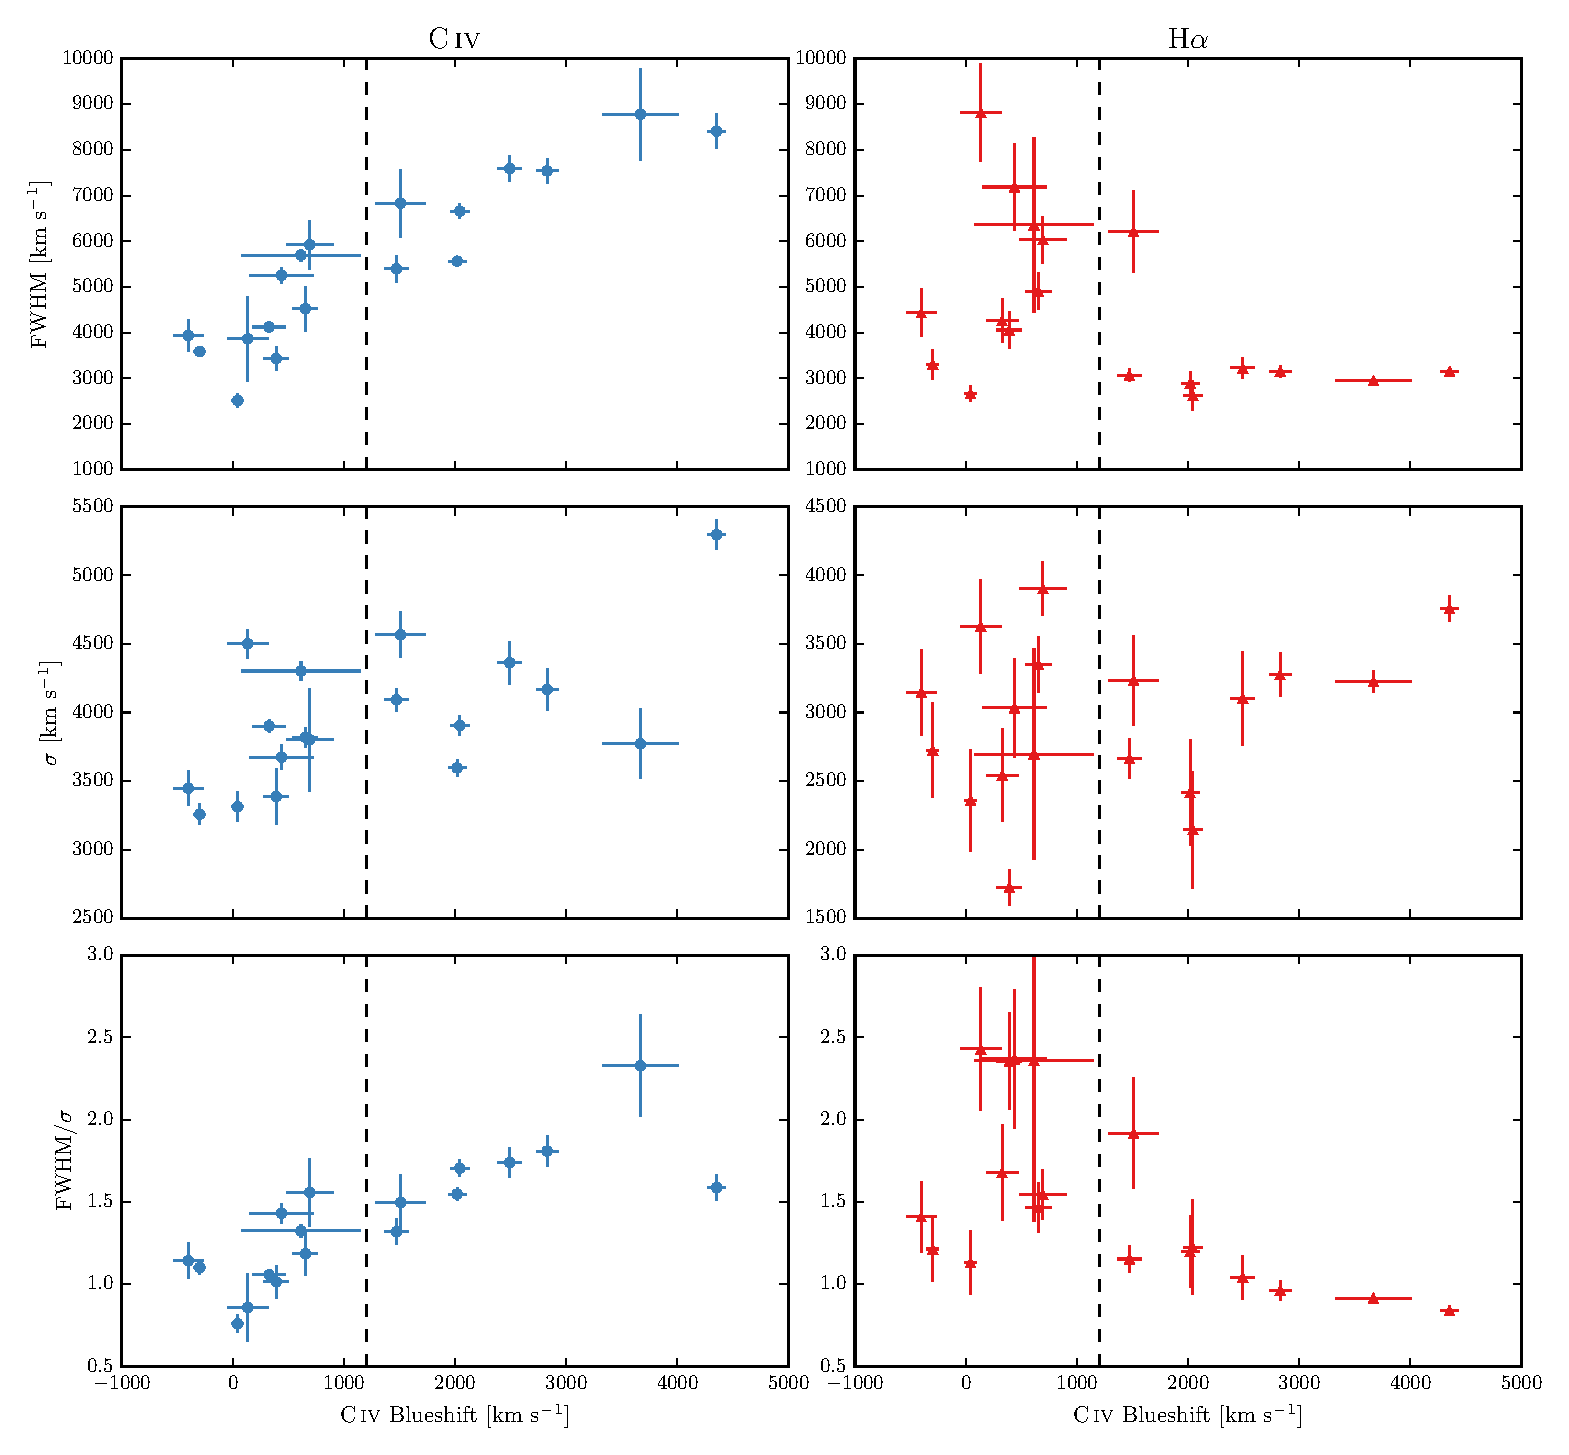
\includegraphics[width=2\columnwidth]{figures/chapter02/civ_ha_comparisons.pdf} % ComparePeaksAll() in reduction_v12.py
    \caption{The FWHM, dispersion ($\sigma$) and shape (FWHM/$\sigma$) of \ion{C}{IV} and \ha as a function of the \ion{C}{IV} blueshift. The vertical line demarcates the `high' and `low' \ion{C}{IV} blueshift regimes discussed in the text. At high blueshift it is clear that BH masses estimated from the \ion{C}{IV} FWHM (as is typically done at the redshifts considered) will be significantly larger than those estimated from the \ha FWHM.}
    \label{fig:line_comparison}
\end{figure*} 

There has been a considerable degree of attention paid to the effectiveness of different velocity-width measures of the \ion{C}{IV}-emission; specifically, the line FWHM and the dispersion, $\sigma$, derived from the second-moment velocity \citep[e.g.][]{assef11, denney13}.
The FWHM and line dispersion trace different parts of the broad line velocity field, with the FWHM relatively more sensitive to any low-velocity core present and the line dispersion relatively more sensitive to the high velocity wings. 
The shape of the line can be characterised by the ratio FWHM/$\sigma$. 
FWHM/$\sigma$ $\simeq 2.35$ for a Gaussian profile, while FWHM/$\sigma$ $\simeq 1$ for a peakier Lorentzian profile\footnote{Strictly FWHM/$\sigma$ $\rightarrow 0$ for a Lorentzian profile, but values close to unity are typical when the dispersion is calculated over a velocity range, $\simeq\pm10\,000$\kms, used to parametrize broad emission lines in quasar spectra.}.
In practice, the line dispersion is almost certainly a more robust velocity indicator when the assumptions underlying the virial-origin of the emission-line velocity width are true and the spectral S/N and resolution are adequate.
This was demonstrated by \citet{denney13} for a sample of quasars possessing a significantly smaller range in \ion{C}{IV}-blueshift than investigated here.

In reality, however, as highlighted by \citet{denney12}, contributions to the \ion{C}{IV}-emission line profile from gas where virial motions do not dominate can be significant. 
Looking to the future, the results of the new reverberation-mapping projects \citep{shen15, kingoz15} will show what fraction of the \ion{C}{IV}-emission line, as a function of velocity, does reverberate for quasars with an extended range of \ion{C}{IV}-emission shapes. 
The derivation of quantitative corrections to transform velocity-width measures from single-epoch to reverberation-only line profiles should then be possible. 

As such information is not yet available, there is a strong rationale for investigating whether the systematic changes in the \ion{C}{IV}-emission line profile can be used to improve the single-epoch BH-mass estimates derived using the \ion{C}{IV} line. 
In the left panels of Fig.~\ref{fig:line_comparison} we show how the \ion{C}{IV} FWHM, line dispersion, $\sigma$, and line shape, FWHM/$\sigma$, vary as a function of the blueshift. 
The \ion{C}{IV} FWHM is correlated with the blueshift, with the median FWHM of quasars with the largest blueshifts a factor of 2-3 higher than quasars with only moderate blueshifts.
The dispersion, however, does not show a similarly strong systematic variation. 

Without knowledge of the \ion{C}{IV}-blueshifts, the dynamic range present in the FWHM and line dispersion measurements accords with the expectations from the study of \citet{denney13}; the factor of $\simeq$4 spread in the FWHM measurements indicating greater sensitivity to the emission-line profile shape than is the case for the dispersion, which varies by a factor of only $\simeq$2. 
Adopting a value of 1200\,\kms\, to define `low' and `high' blueshift, the median \ion{C}{IV}-emission dispersion for the low and high-blueshift samples differ by only 10 per cent. 
It follows, therefore, that while the dispersion provides a relatively line-profile independent measure of the velocity width for quasars where the underlying assumption regarding the virial-origin of the velocity width applies, quasars where the assumption is not true can be assigned apparently normal velocity-widths and hence potentially incorrect BH-masses. 

To emphasise this point, in Fig.~\ref{fig:civ_comparison} we overlay the \ion{C}{IV} line profiles of SDSSJ1236+1129 and SDSSJ1525+2928, whose dispersions (Table~\ref{tab:emissionproperties}) are indistinguishable (4168$\pm$271 and 4303$\pm128$\,\kms respectively). 
Notwithstanding the very similar dispersion values, the emission-line velocity fields differ dramatically and, therefore, the dispersion values cannot be measuring accurately the virial-induced velocity spread of the \ion{C}{IV} emission in both quasars.

The analysis here, building on earlier work \citep[including][]{shen12, sulentic07}, confirms a link between \ion{C}{IV} emission-line shape and blueshift, raising the prospect of developing a blueshift-dependent correction to single-epoch BH-mass estimates based on the \ion{C}{IV} line. 
Expressed in another way, we are interested in testing if the significant systematic change in line shape as a function of \ion{C}{IV} blueshift can be used to provide improved single-epoch BH-masses from the \ion{C}{IV} emission line.  
The tightness of the correlation we observe between the \ion{C}{IV} FWHM and blueshift implies that such an approach may be more effective than using the \ion{C}{IV} emission-line velocity dispersion without reference to blueshifts.
A further practical advantage is that, given the typical S/N of current survey-quality spectra, virial BH mass estimates for high-redshift quasars are usually based on the FWHM rather than the dispersion \citep[e.g.][]{shen11}, which, being strongly affected by the continuum placement, is often found to be difficult to measure robustly \citep[e.g.][]{mejia-restrepo16}. 
As a first step towards the goal, below (Sec.~\ref{sec:hatrends}) we investigate the apparent systematic trends in the \ha FWHM and line shape as a function of \ion{C}{IV} blueshift (shown in the right of Fig.~\ref{fig:line_comparison}).

\begin{figure}
	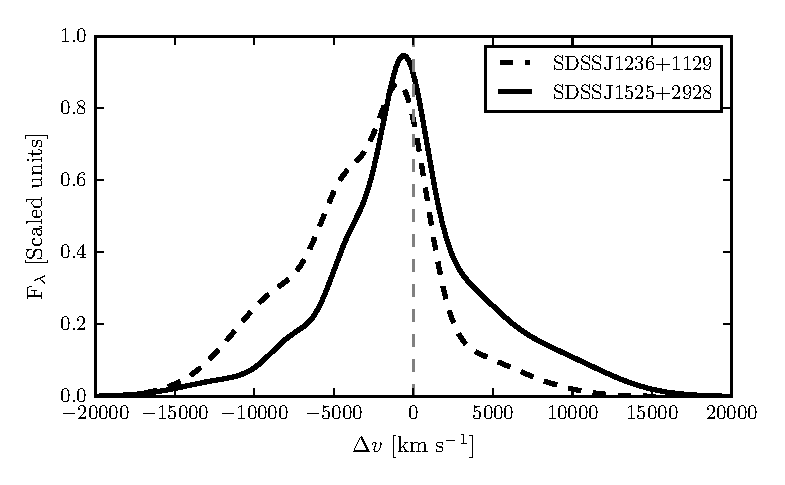
\includegraphics[width=\columnwidth]{figures/chapter02/civ_comparison.pdf} 
    \caption{Comparison of the \ion{C}{IV} line profiles of SDSSJ1236+1129 and SDSSJ1525+0426. Notwithstanding the essentially identical dispersion values, the emission-line velocity fields differ dramatically and, therefore, the dispersion values cannot be measuring accurately the virial-induced velocity spread of the \ion{C}{IV} emission in both quasars. }
    \label{fig:civ_comparison}
\end{figure}

\subsection{Computing BH mass estimates}
\label{sec:nonvirialmass}

Single-epoch virial BH mass estimates normally take the form

\begin{equation}
  \label{eq:virialmass}
  {\rm M_{BH}} = 10^{a} \left( \frac{\Delta V}{1000~{\rm km~s^{-1}}} \right)^b \left[ \frac{L_{\lambda}}{10^{44}~{\rm erg~s^{-1}}} \right]^c
\end{equation}

\noindent where $\Delta V$ is a measure of the line width (from either the FWHM or dispersion), $L_\lambda$ is the monochromatic continuum luminosity at wavelength $\lambda$, and $a$, $b$, and $c$ are coefficients, determined via calibration against a sample of AGN with reverberation-mapping BH mass estimates. Several calibrations have been derived using different lines (e.g. \hbns, \ion{Mg}{II}, \ion{C}{IV}) and different measures of the line width (FWHM or dispersion) \citep[e.g.][]{vestergaard02,mclure02,vestergaard06,mcgill08,wang09,rafiee11,park13}.

Reverberation mapping measurements of nearby AGN have revealed the BLR to be stratified, with high-ionisation lines, including \ion{C}{IV}, emitted closer to the BH than low-ionisation lines, including \ha and \hb \citep[e.g.][]{onken02}.
\citet{vestergaard06} found that the \ion{C}{IV}-emitting region is at approximately half the radius of the \hbns/\ha emitting region.
Given the $\Delta V \propto R_{\rm BLR}^{-0.5}$ virial relation, this leads to the prediction that the \ion{C}{IV} line widths should be $\simeq 1.4$ times broader than \ha for a given BH mass. 
More recently, \citet{denney12} found that there is a significant contribution from gas at larger radii to the \ion{C}{IV} emission line, enhancing the profile at lower-velocity and leading to smaller FWHM or dispersion values. 
The ratio of the line widths is therefore predicted to be lower than the factor of $\simeq 1.4$. 

An alternate virial BH-mass calibration is proposed by \citet{park13}, using an improved sample of AGN with reverberation mapped masses. 
A major difference from the calibration of \citet{vestergaard06} is that \citet{park13}, recognising the poor correlation sometimes observed between the \ion{C}{IV} and \hb FHWM, allow the exponent on the velocity width ($b$ in Eq.~\ref{eq:virialmass}) to vary.
Calibrating Eq.~\ref{eq:virialmass} against reverberation BH masses, they find a best-fit value of $b=0.56$, which is much less than the $b=2.0$ in the strict virial regime. 
As a result, the derived BH masses are much less sensitive to the \ion{C}{IV}-emission line properties.
By contrast our approach is to investigate whether a more complete parametrization of the \ion{C}{IV}-emission profile can be used to improve BH-mass estimates based on the conventional virial relation, with $b=2.0$.

\subsection{\ion{C}{IV}-derived BH masses at low \ion{C}{IV} blueshift}
\label{sec:bhm_lowbs}

The \ha and \ion{C}{IV} FWHM (dispersion) of the 10 quasars with \ion{C}{IV} blueshifts $<$1200\,\kms\, are linearly correlated, as expected if the dynamics of the BLR clouds are dominated by virial motions. 
The median \ion{C}{IV}/\ha FWHM (dispersion) ratio is 0.91 (1.22) with standard deviation 0.17 (0.28). 
Thus, the dispersion-based comparison results in a median \ion{C}{IV}/\ha consistent with the value of $\simeq1.4$ from assuming a virial origin for the emission but with a relatively large standard deviation. 
As predicted in Section~\ref{sec:nonvirialmass}, the FWHM-based comparison results in a systematically lower median \ion{C}{IV}/\hans.
However, the correlation between the \ion{C}{IV} and \ha FWHMs is significantly tighter, lending support to the proposal that corrections to BH-mass estimates based on the \ion{C}{IV} emission line properties may be possible.

Virial BH masses were calculated using the widely adopted \citet{vestergaard06} calibrations. 
The \citet{vestergaard06} \ion{C}{IV} FWHM calibration uses the monochromatic continuum luminosity at 1350\,\AA\, to predict the BLR radius and corresponds to ($a=6.66$, $b=2$, $c=0.53$) in Eq.~\ref{eq:virialmass}. 
The calibration coefficient $a=6.73$ in their equivalent dispersion-based relation. 
For the \hb calibration, \citet{vestergaard06} use the monochromatic continuum luminosity at 5100\,\AA\, and calibration coefficients corresponding to ($a=6.91$, $b=2$, $c=0.5$).
BH masses are computed using the line and continuum properties given in Tables \ref{tab:emissionproperties} and \ref{tab:continuumproperties}, and we convert our \ha emission-line velocity-width measures to predicted \hb widths using Eq.~\ref{eq:hb2hawidth}.

As a direct consequence of the empirically small \ion{C}{IV}/\ha FWHM ratio, the \ion{C}{IV}-derived BH mass estimates are systematically lower than the corresponding \hans-derived masses when the blueshift is small.
This can be seen in Fig~\ref{fig:bhm_blueshift}, where for every quasar with a \ion{C}{IV} blueshift $<$1200\,\kms (i.e. to the left of the dashed line), the \ion{C}{IV}-derived BH mass is smaller than the corresponding \hans-derived mass.
The median fractional difference between the two estimates is 0.60.  

\begin{figure}
	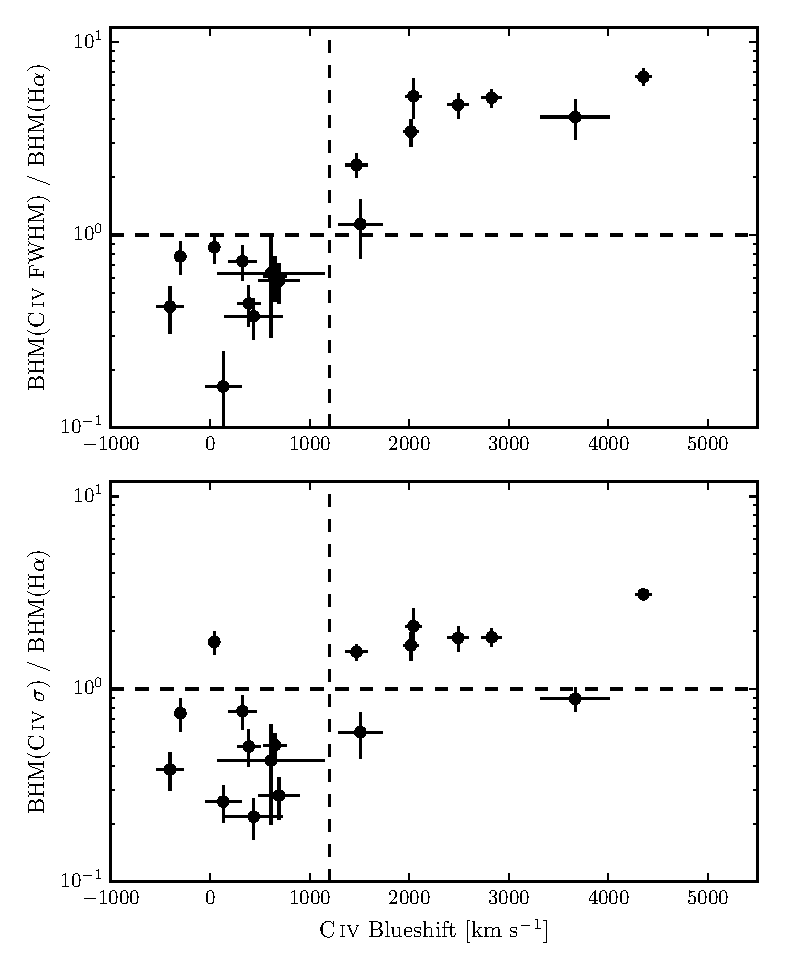
\includegraphics[width=\columnwidth]{figures/chapter02/bs_bhm.pdf}
    \caption{Comparison of virial BH mass estimates based on the \ion{C}{IV} FWHM ({\it top}) and dispersion $\sigma$ ({\it bottom}) and \ha FWHM as a function of the \ion{C}{IV} blueshift. The horizontal line indicates agreement between \ion{C}{IV} and \ha BH masses, and the vertical line demarcates the `high' and `low' \ion{C}{IV} blueshift regimes discussed in the text. The BH masses of quasars with moderate \ion{C}{IV} blueshifts are underestimated when using the \ion{C}{IV} FWHM, while the masses of quasars with large blueshifts are severely overestimated. This situation cannot be corrected by changing the exponent on the FWHM \citep[e.g.][]{rafiee11,park13} or the overall scaling in standard virial BH mass relations.}
    \label{fig:bhm_blueshift}
\end{figure}

For the 10 quasars with low \ion{C}{IV} blueshifts, we looked for correlations of the \ion{C}{IV}/\ha FWHM ratio with other spectral properties.
We found marginal evidence for an anti-correlation with the \ha FWHM (Spearman coefficient 0.58 with p-value 0.08). 
Among the quasars with \ha FWHM $>4000$\kms we found the mean \ion{C}{IV}/\ha FWHM ratio to be 0.83, compared to 1.01 for the quasars with \ha FWHM $<4000$\kms.  
Similar trends have been observed at low-$z$; in a sample of \citet{boroson92} quasars, \citet{baskin05} found the \ion{C}{IV} line to be broader than \hb when the \hb FWHM $<$4000 \kms and narrower when the \hb FWHM $>$4000 \kms. 

\subsection{\ion{C}{IV}-derived BH masses at high \ion{C}{IV} blueshift}
\label{sec:highzmasses}

In Section~\ref{sub:charemprof} we have shown that the \ion{C}{IV} emission at large \ion{C}{IV}-blueshift is not dominated by virial-induced motions due to the BH. 
The empirically derived increase in the \ion{C}{IV} emission FWHM with blueshift leads directly to an overestimate of BH-mass if the trend with blueshift is not taken into account. 
The availability of the \hans-spectra for the sample allows the quantification of the bias in inferred BH-mass under the assumption that the \ha emission line provides a reliable BH mass. 

Figure~\ref{fig:bhm_blueshift} shows the ratio of the \ion{C}{IV}- and \hans-FWHM derived BH masses as a function of the \ion{C}{IV} blueshift.  
We see that for quasars with \ion{C}{IV} blueshifts $>2000$\,\kms, the \ion{C}{IV}-based masses overestimate the \hans-based masses by as much as a factor of $\sim$5. 

The existence of a trend in the \ion{C}{IV}-dispersion values with \ion{C}{IV} blueshift is evident from inspection of the bottom left panel of Fig.~\ref{fig:line_comparison} but the systematic trend relative to the spread at fixed blueshift is significantly smaller than when using \ion{C}{IV} FWHM. 
Similarly, Fig.~\ref{fig:bhm_blueshift} shows, at most, only a weak increase in the ratio of \ion{C}{IV}- and \hans-derived masses. 
Without knowledge of the \ion{C}{IV} blueshifts the distribution of \ion{C}{IV}- and \hans-dispersion based BH masses could be taken to be reassuring. 
Including the \ion{C}{IV}-blueshift information, however, demonstrates that any such interpretation is inherently flawed because the origin of the \ion{C}{IV} emission velocity width is not due to virial-motions for a significant range of \ion{C}{IV} blueshift. 
To reiterate the point made above (Sec.~\ref{sub:charemprof}), we believe that using a greater knowledge of the line profile (i.e. both the FWHM and blueshift) is a better motivated (and more practical) approach to obtaining more reliable virial BH mass estimates from the \ion{C}{IV} line. 

The number of objects in our sample is small but an important factor contributing to the significant correlation evident in the FWHM version of Fig.~\ref{fig:bhm_blueshift} is a change in the emission-line shape of \ha as the \ion{C}{IV}-blueshift increases.
By comparing the distributions of the \ha FWHM and dispersion as a function of \ion{C}{IV}-blueshift (shown in the right-panels of Fig.~\ref{fig:line_comparison}), there is trend for the \ha lines to become peakier (with FWHM/$\sigma$ approaching unity) as the \ion{C}{IV} blueshift increases. 
Whether the size of the true systematic bias in BH masses inferred from \ion{C}{IV}-emission FWHM is as large as shown in Fig.~\ref{fig:bhm_blueshift} will depend on the future parametrization of the reverberation-component present in \hb (and \hans) profiles for quasars with high luminosities and large \ion{C}{IV} blueshifts.

In summary, Fig.~\ref{fig:bhm_blueshift} illustrates the extent to which key derived physical parameters, including the BH mass and $L/L_{\rm Edd}$, could be systematically in error when \ion{C}{IV}-FWHM measures are used without incorporating the information from the \ion{C}{IV} blueshifts. 
Other authors have proposed empirical corrections to \ion{C}{IV}-based BH masses based on similar systematic trends seen in the \ion{C}{IV} line shape \citep{denney12} and the continuum-subtracted peak flux ratio of the ultraviolet emission-line blend of \ion{Si}{IV}+\ion{O}{IV} (at 1400\,\AA) to that of \ion{C}{IV} \citep{runnoe13}.
In Section~\ref{sec:discussionbiases} we apply these corrections the quasars in our sample, and discuss the effect they have on the systematic bias seen in Fig.~\ref{fig:bhm_blueshift}. 

\subsection{Population trends with \ion{C}{IV} blueshift}
\label{sec:hatrends}

\begin{figure}
	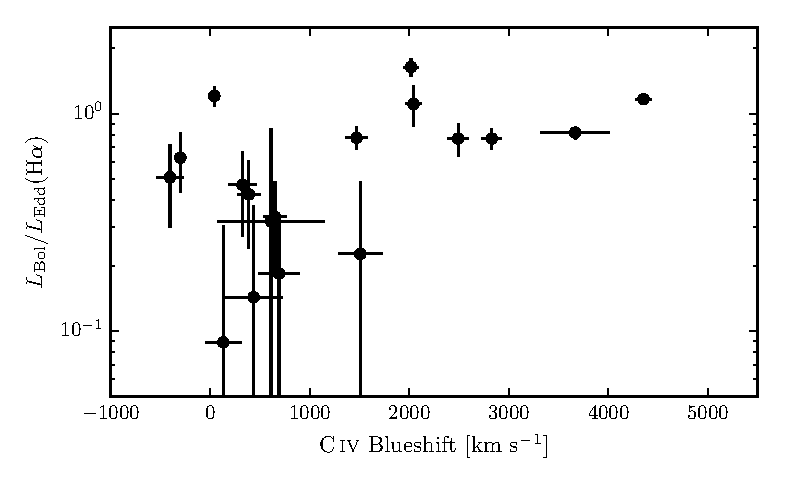
\includegraphics[width=\columnwidth]{figures/chapter02/ha_edd_civ_bs.pdf}
    \caption{\hans-derived Eddington ratio versus \ion{C}{IV} blueshift. At blueshift $\gtrsim$ 2000\kms\, all quasars have high accretion rates ($L/L_{\rm Edd} \simeq 1$). This is in agreement with \citet{kratzer15}, but in contrast to what one would derive from naive use of \ion{C}{IV}-based BH mass scaling relations.}
    \label{fig:ha_edd_civ_bs}
\end{figure}

Even with the caveat regarding the small sample size, the differences in the \ha emission-profile as a function of \ion{C}{IV}-blueshift (Fig.~\ref{fig:gridspectra_1}) appear to be systematic.
At \ion{C}{IV}-blueshift $<$1200\,\kms, the \ha FWHM range is $\simeq2700 - 8800$\,\kms, with mean $\simeq$5200\,\kms.
However, amongst the six quasars with \ion{C}{IV}-blueshift $>$2000\,\kms, the mean \ha FWHM=3000\,\kms, with a scatter of just 200\,\kms. 
The apparent trend of peakier \hans-emission, with FWHM/$\sigma$ close to unity, at large \ion{C}{IV}-blueshift is enhanced by the modest increase in \ha EW with blueshift (Table~\ref{tab:emissionproperties}). 
Amongst the low-\ion{C}{IV}-blueshift population there are in addition quasars with broader and more Gaussian-like \ha line profiles, with FWHM/$\sigma \simeq 2$ . 

The change in the \ha emission-line profiles as a function of \ion{C}{IV}-blueshift means that the \hans-FWHM derived BH masses at high-blueshift are smaller than the sample mean. 
We transformed the observed luminosity into a mass-normalised accretion rate (Eddington ratio).
To convert the monochromatic luminosity, which is observed, in to a bolometric luminosity we use the bolometric correction factor given by \citet{richards06} ($L_{\rm bol} = 9.26L_{5100}$).
Although there is evidence that the bolometric correction factor is a function of the luminosity, as well as of other parameters including the \ion{C}{IV} blueshift \citep{krawczyk13}, the differences are small over the parameter range covered by our sample, and for simplicity we adopt a constant factor. 

The results, shown in Fig.~\ref{fig:ha_edd_civ_bs}, show that at large blueshifts quasars are accreting at around their Eddington limits (Fig.~\ref{fig:ha_edd_civ_bs}). 
The converse is, however, not true, i.e. not all quasars with high Eddington ratios possess large \ion{C}{IV} blueshifts \citep[see][]{baskin05}.

\section{Discussion}
\label{sec:discussion}

\subsection{Biases in single-epoch \ion{C}{IV}-based BH-mass estimates}
\label{sec:discussionbiases}

The \ion{C}{IV} line profiles of the quasars with  the largest \ion{C}{IV} blueshifts (in the bottom right of Fig.~\ref{fig:civ_space}) demonstrate that non-virial motions are having a significant effect on the \ion{C}{IV} BLR dynamics. 
At fixed emission-line EW, almost the entire \ion{C}{IV}-profile appears to shift blueward and the change in line shape is not simply an enhancement of flux in the blue wing of a symmetric component. 
It is clear that the virial assumption, on which single-epoch BH-mass measurements are predicated, is not straightforwardly applicable for the \ion{C}{IV}-emission line in quasars exhibiting large blueshifts. 

Quantitatively, the \ion{C}{IV}-shape change is most apparent from the FWHM values, which are strongly correlated with the \ion{C}{IV}-blueshift. 
This trend has previously been identified, by comparison with \ion{Mg}{II} at lower-redshifts \citep{shen08,shen11} and \hb at higher redshifts \citep{shen12}.
We find that virial BH mass estimates based on the \ion{C}{IV} FWHM will overestimate the true mass by a factor of $\sim$5 for objects exhibiting the largest \ion{C}{IV} blueshifts. 

In contrast, the \ion{C}{IV} line dispersion does not show a similarly strong dependence on the blueshift. 
This is a result of the shape of the \ion{C}{IV} line profile being dependent on the blueshift; the low-blueshift profiles are peakier (FWHM/$\sigma \simeq 1$) than the high-blueshift profiles (FWHM/$\sigma \simeq 2$). 
\citet{denney12} found the level of contamination in single-epoch spectra from non-reverberating gas to be correlated with the shape (FWHM/$\sigma$) of the \ion{C}{IV} profile. 
Their investigation was based on a sample of reverberation mapped quasars, which have a narrow range of \ion{C}{IV}-emission line shapes, including the absence of any objects with large \ion{C}{IV} blueshifts. 
The FWHM/$\sigma$-based correction to the \ion{C}{IV} FWHM proposed by \citet{denney12} increases the inferred BH masses by $\sim$0.2 dex at the low end of our \ion{C}{IV} blueshift distribution, thereby reducing part of the systematic trend in the BH mass (Fig.~\ref{fig:corrections}).  
However, it is not applicable at the high \ion{C}{IV} blueshift end, where velocity widths are likely dominated by non-virial motions.
Based on the typical line shape of \ion{C}{IV} in these high-blueshift quasars (FWHM/$\sigma \simeq 2$), the \citet{denney12} correction decreases the predicted BH masses by $\sim$0.3 dex, which has only a moderate decreasing effect on the strong systematic (Fig.~\ref{fig:corrections}).  

While the \ion{C}{IV}-line dispersion is largely independent of the blueshift, it does not follow that dispersion-based BH-mass estimates are correct, because the underlying assumption regarding the virial-origin of the \ion{C}{IV} emission profile breaks down at large blueshifts.
Furthermore, given the difficulty in obtaining reliable dispersion measurements from survey-quality spectra with limited S/N \citep[e.g.][]{mejia-restrepo16}, virial BH-mass estimates for existing large samples of high-redshift quasars are usually based on the FWHM \citep[e.g.][]{shen11}. 
Our work therefore suggests that a viable recipe for obtaining more reliable BH mass estimates for large numbers of quasars at high redshift is to measure both the FWHM and the blueshift, which together can be used to derive a FWHM corrected for the non-virial contribution. 

Although we do not have enough quasars in our sample to derive a reliable quantitative correction to BH-masses as a function of \ion{C}{IV} blueshift, we are assembling a large sample of quasar spectra with coverage of both \ion{C}{IV} and \hbns/\ha in order to empirically validate such a correction. 
Both \citet{runnoe13} and \citet{shen12} considered a similar approach, but concluded that a low-ionisation broad line (e.g. \ion{Mg}{II}), or features from the quasar NLR, are required to determine the systemic redshift and hence the \ion{C}{IV} blueshift. 
Empirical tests of the reliability of the improved \citet{hewett10} redshifts for the SDSS DR7 quasars \citep{shen16b} and the availability of the largely SED-independent principal component analysis redshifts for DR10 and DR12 \citep{paris14, paris17} already allow meaningful corrections to BH-mass estimates for quasars exhibiting large \ion{C}{IV}-blueshifts.
Our intention is, however, to determine a definitive correction formula using the redshifts from Allen \& Hewett (2016, in preparation) for both DR7 and DR12.

Given the difficulty of measuring reliable \ion{C}{IV} blueshifts, \citet{runnoe13} opted instead to use the continuum-subtracted peak flux ratio of the ultraviolet emission-line blend of \ion{Si}{IV}+\ion{O}{IV} (at 1400\,\AA) to that of \ion{C}{IV} to correct for non-virial contributions to the \ion{C}{IV} velocity width. 
This parameter was chosen because it showed the strongest correlation with the FWHM \ion{C}{IV}/\hb residuals, as well as with the strengths of optical \ion{O}{III} and \ion{Fe}{II}. 
The strengths of optical \ion{O}{III} and \ion{Fe}{II}, being parameters in EV1, are also correlated with the \ion{C}{IV} blueshift \citep{sulentic07}. 
As the \ion{C}{IV} blueshift increases the EW decreases systematically (Fig.~\ref{fig:civ_space}).
The \ion{Si}{IV}+\ion{O}{IV} emission-line blend, however, shows significantly less systematic variation. 
Therefore, while the \citet{runnoe13} \ion{Si}{IV}+\ion{O}{IV}-based correction is effective in practice, the \ion{C}{IV} blueshift measurement provides a more direct measure of the non-virial contributions to the \ion{C}{IV} velocity width.

In our sample, we find the 1400\,\AA/\ion{C}{IV} peak flux ratio to be strongly correlated to the \ion{C}{IV} blueshift (the Spearman coefficient for the correlation is 0.82, $p$-value 2{\sc e}-5).
As such, the correction to \ion{C}{IV}-based virial masses proposed by \citet[][their equation 3]{runnoe13} removes a large part of the systematic in the \hans/\ion{C}{IV} FWHM residuals with the \ion{C}{IV} blueshift (Fig.~\ref{fig:corrections}); the median \ion{C}{IV}/\ha FWHM ratio at large \ion{C}{IV} blueshifts ($>$1200\kms) is reduced from 4.5 to 1.5.
However, at low ($<$1200\kms) \ion{C}{IV} blueshifts, the trend for \ion{C}{IV} to predict lower BH masses persists, and the scatter between the \ion{C}{IV}- and \hans-based masses increases by a factor of two.   
In accordance with our expectations, we find the FWHM \ion{C}{IV}/\ha residuals to be more tightly correlated to the \ion{C}{IV} blueshift (Spearman coefficient 0.82, $p$-value 3{\sc e}-5) than to the 1400\,\AA/\ion{C}{IV} peak flux ratio (Spearman coefficient 0.72, $p$-value 7{\sc e}-4). 

\begin{figure}
	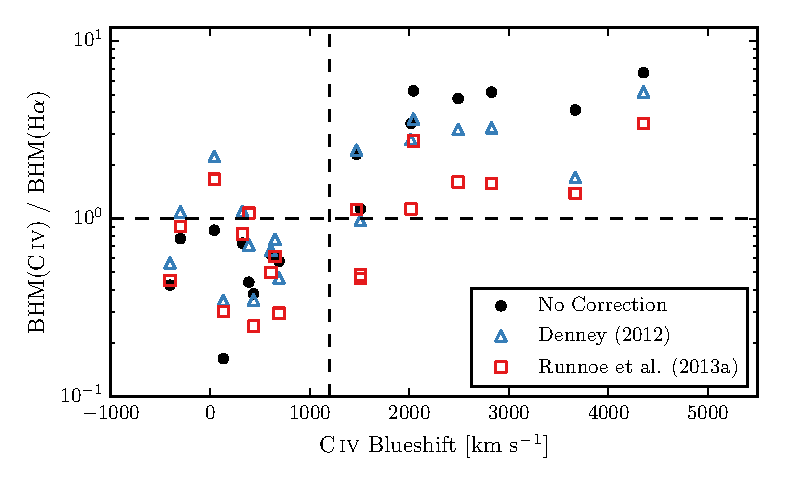
\includegraphics[width=\columnwidth]{figures/chapter02/corrections.pdf}
    \caption{Comparison of BH mass estimates derived from the FWHM of \ion{C}{IV} and \ha as a function of the \ion{C}{IV} blueshift (\textit{black circles}), and after applying corrections to the \ion{C}{IV}-derived mass based on the line shape \citep[\textit{blue triangles};][]{denney12} and the peak flux ratio of the \ion{Si}{IV}+\ion{O}{IV} blend relative to \ion{C}{IV} \citep[\textit{red squares};][]{runnoe13}. While the shape-based correction improves the consistency between BH mass estimates in the low-blueshift population, only the \ion{Si}{IV}+\ion{O}{IV}/\ion{C}{IV} peak flux-based correction is effective at high blueshifts (although a weak systematic remains).}
    \label{fig:corrections}
\end{figure}

\subsection{Possible systematic trends in \ha BH-mass estimates}

In Section~\ref{sec:hatrends}, we found that the quasars with large \ion{C}{IV} blueshifts have systematically narrower \ha FWHM (Fig.~\ref{fig:line_comparison}).
Using the standard virial BH mass calibrations this implies that the high \ion{C}{IV} blueshift population have high accretion rates ($L/L_{\rm Edd} \simeq 1$; Fig.~\ref{fig:ha_edd_civ_bs}). 
This interpretation requires some caution since the emission-line shape (characterized by the value of FWHM/$\sigma$) of \ha is also changing as a function of the \ion{C}{IV} blueshift (Fig.~\ref{fig:line_comparison}). 
At low \ion{C}{IV} blueshifts there are a range of shapes, but all of the quasars exhibiting large \ion{C}{IV} blueshifts have peaky \ha profiles with FWHM/$\sigma \simeq 1$. 
This raises the question of whether the \ha FWHM is a reliable proxy for the virial-induced velocity dispersion for the full range of \ha line shapes we have in our sample. 

When calibrating the virial-product to masses derived independently using the BH mass \---\ stellar velocity dispersion ($M_\odot-\sigma$) relation, \citet{collin06} find that the scaling factor, $f$, is a factor $\sim2$ larger for their Population `1' sources (with FWHM/$\sigma < 2.35$ and essentially equivalent to population A of Sulentic and co-workers and to the high-blueshift quasars here) than for their Population 2 (with FWHM/$\sigma > 2.35$). 
For single-epoch BH-mass estimates, assuming a constant value of $f$, as is normally done \citep[e.g.][]{vestergaard06}, means that Population 1 masses will be underestimated and Population 2 will be overestimated.
In the context of this result from \citet{collin06}, our high-blueshift objects all possess peaky \hans-lines and, while our quasar sample probes much higher luminosities and masses, the true BH-masses may also be underestimated.
Adopting such an interpretation, the amplitude of the trend seen in Fig.~\ref{fig:bhm_blueshift} might not be so pronounced.

As mentioned in Section~\ref{sec:introduction} and discussed in \citet{richards11}, quasars with current reverberation mapping measurements have a restricted range of \ion{C}{IV}-line shapes. 
There are currently very few reverberation-mapping measurements of quasars with large \ion{C}{IV} blueshifts but the results of the large on-going statistical reverberation mapping projects \citep[e.g.][]{shen15} for luminous quasars at high-redshift will go some way to establishing whether the quasar broad line regions producing Balmer emission look the same for objects with very different \ion{C}{IV}-emission blueshifts. 

Although the EV1-trends \citep{sulentic00b,shen14} are most likely driven by the accretion rate, orientation may also have a role to play in determining the observed properties of the BLR. 
\citet{shen14} argue that a large part of the scatter observed in the \hb FWHM relates not to a spread in BH masses, but rather to the orientation of the BLR relative to the line-of-sight.
For this to be true, the BLR would need to be in a flattened disc-like geometry, in which case the observed line width would increase with the inclination of the disc relative to the line of sight. 
\citet{brotherton15b} found that the core-dominance of radio-loud quasars, which is believed to be a reliable proxy for orientation, at least in a statistical sense, is significantly correlated with the \hb FWHM and hence with the BH-mass estimates. 
This raises the question of whether the narrow \ha emission lines observed in the quasars with the largest \ion{C}{IV} blueshifts could be an orientation effect. 
However, there is no evidence that the \ion{C}{IV} blueshift is dependent on the orientation \citep[inferred from the radio core-dominance;][]{richards11,runnoe14}. 
Furthermore, \citet{leighly04} showed that the \ion{He}{II}\l1640 emission-line properties of quasars with large \ion{C}{IV} blueshifts are more consistent with differences in the SED rather than differences in the orientation.
\citet{collin06} showed that orientation effects were also sub-dominant to the Eddington ratio in determining the shape of the \hb line and
the \ha line shape trend we observe is consistent with the finding of \citet{marziani03} that the \hb emission profiles of high/low Eddington ratio low-$z$ quasars and type 1 Seyfert nuclei are well fit by Lorentzian and double Gaussian profiles respectively.  
Overall, therefore, orientation does not appear to be the dominant effect in determining the \ion{C}{IV} blueshift and correlated changes in the \ha line profile. 

\subsection{Accretion-rate trends in the quasar population}

The blueshifting of \ion{C}{IV} is usually interpreted as evidence for strong outflows resulting from the presence of a radiation-driven accretion-disc wind. 
\citet{richards02} found that quasars with large \ion{C}{IV} blueshifts have weak \ion{He}{II}.
This is evidence for weak soft X-ray continuum emission \citep{leighly04}, which would allow a strong line-driven wind to form.  
The strength of such a wind is predicted to be related to the quasar far-ultraviolet SED, which, in turn, could be related to the mass-accretion rate.
This picture is therefore consistent with our finding that the quasars with large \ion{C}{IV} blueshifts have high accretion rates. 

All of the objects in our sample which exhibit large \ion{C}{IV} blueshifts would be classified as population A in the \citet{sulentic00b} scheme based on the \ha FWHM (see Section~\ref{sec:introduction}). 
Our results therefore support the idea of the \citet{sulentic00b} A/B division being driven by the Eddington ratio, with population A sources possessing higher accretion rates.
However, we also observe a number of quasars which have high Eddington ratios but do not have line profiles suggestive of strong outflows in the \ion{C}{IV} BLR.  
This suggests that a high accretion rate is a necessary but not sufficient condition for the existence of outflows \citep{baskin05}. 

The two-dimensional nature of the \ion{C}{IV} emission line parametrization and the apparent anti-correlation between \ion{C}{IV} EW and \ion{C}{IV} blueshift suggests that the quasar population exhibits a continuum of properties. 
As such, more accurate \ion{C}{IV} blueshift measurements for SDSS-quasars should allow an improved mapping between the \ion{C}{IV}-emission properties and key physical parameters of the quasars.
This includes improving our understanding of the origin of quasars with exceptionally weak, blueshifted \ion{C}{IV} emission \citep[weak emission line quasars;][]{luo15} which could be exotic versions of wind-dominated quasars \citep{plotkin15}.

\subsection{The BAL parent population}

Classical high-ionization BAL (HiBAL) quasars are also predominantly Population A objects in the scheme of \citet{sulentic00b}. 
There are no HiBAL quasars in our sample by design (Section~\ref{sec:selection}) but it is generally accepted that quasars which show high-ionisation BALs are likely to be radiating with relatively high $L/L_{\rm Edd}$ \citep[e.g.][]{zhang14}. 
We therefore propose that the subset of the quasar population that exhibits large \ion{C}{IV}-emission blueshifts, with high-EW and narrow-\ha emission lines, may be directly related to the HiBAL quasar population \---\ perhaps even the `parent' population \citep{richards06conf}. 
A prediction of such a linkage is that near-infrared observations of the rest-frame optical spectra of HiBAL quasars will show strong, relatively narrow, Balmer emission lines, very similar to those of the quasars with high \ion{C}{IV}-blueshifts presented in this paper \citep[see][for such a study]{runnoe13b}. 

\subsection{The frequency of quasars with high accretion rates}

Quantifying the frequency of quasars producing outflows as a function of key parameters, e.g. quasar luminosity, BH-mass, redshift,... will be important to constrain models of quasar-galaxy evolution.  
At fixed BH mass, the intrinsic and the observed fraction of quasars exhibiting properties that depend on the Eddington ratio can differ significantly. 
As an illustration, we consider the implications for the intrinsic fraction of quasars possessing large \ion{C}{IV} blueshifts given the observed numbers in the $m_i<19.1$ flux-limited sub-sample of the SDSS DR7 quasar catalogue, from which our quasar sample is effectively drawn (Section~\ref{sec:selection}). 
In order to estimate the size of the selection effect, we considered the detection probability for a much-simplified quasar population. 
We assume that all quasars with \ion{C}{IV} blueshifts $>$1200\,\kms have enhanced accretion rates relative to the `normal' population (with \ion{C}{IV} blueshifts $<$1200\,\kms). 
If the accretion rate of the high-blueshift population is double the rate of the low-blueshift population (which is true in an average sense \---\ see Fig.~\ref{fig:ha_edd_civ_bs}), then the high-blueshift population will be brighter by $\simeq$0.75 magnitude.
Under the assumption that the BH mass distribution is independent of the \ion{C}{IV} blueshift, the high-blueshift population will then be over-represented in a flux-limited sample.
To estimate the size of the bias, we need to know how many more quasars, at redshifts $2 < z < 2.5$, there are with $m_i<19.1+0.75=19.85$ relative to $m_i < 19.1$.
This is the fraction of the population which, as a consequence of having enhanced accretion rates, are boosted above the survey flux limit.    
The main colour-selected SDSS DR7 quasar catalogue extends only to $m_i= 19.1$ and, assuming the luminosity function is continuous\footnote{The luminosity function and number-counts vary only smoothly \citep[e.g.][]{ross13} for the magnitude and redshift range used here.} we thus use the number counts at $m_i < 19.1$ and $m_i < 18.35$, which differ by a factor of $\simeq 4$. 

At redshifts $2 < z <2.5$, there are 3,834 quasars with \ion{C}{IV} blueshifts $<$1200\,\kms and 2,484 with blueshifts $>$1200\,\kms in the SDSS DR7 $m_i < 19.1$ quasar sample, a ratio of $\sim$2:1. 
The above calculation, although much idealised, suggests that the intrinsic fraction of high-blueshift quasars is a factor of four smaller than in the flux-limited sample (i.e. $\sim$15\,per cent of the ultraviolet-selected non-BAL quasar population). 

\section{Conclusions}
\label{sec:conclusions}

We have presented an analysis of biases in \ion{C}{IV}-derived virial BH masses of high-luminosity (L$_{\rm{bol}} \sim$ 47 erg s$^{-1}$) quasars at redshifts $\sim2.5$ from the Sloan Digital Sky Survey. 
Many authors have reported a large scatter between \ion{C}{IV}- and \hans/\hbns-based masses, and part of this scatter has been shown to correlate with the \ion{C}{IV} blueshift \citep{shen12}.
The blueshifting of \ion{C}{IV} is usually interpreted as evidence for strong outflows which, most likely, result from the presence of a radiation line-driven accretion-disc wind. 
Our study is the first to examine this bias systematically across the full range of \ion{C}{IV}-emission line blueshifts observed in the SDSS sample. 
In particular, we have used rest-frame optical spectra of 19 quasars in the redshift range $2 < z < 2.7$ to directly compare \ion{C}{IV} and \ha emission properties as a function of the \ion{C}{IV} blueshift. 
We reach the following conclusions:

\begin{itemize}

\item{A strong correlation between \ion{C}{IV}-velocity width and blueshift is found and at large blueshifts, $>$2000\,\kms, the velocity-widths are dominated by non-virial motions. 
This suggests that the assumption that velocity-widths arise from virial-induced motions, on which single-epoch BH-mass measurements are predicated, is not straightforwardly applicable to these high-blueshift quasars.}

\item{We use the \ha emission line to provide BH-mass estimates that are unbiased by non-virial contributions to the velocity width. 
We find that the \ion{C}{IV}-based BH masses of quasars with low \ion{C}{IV} blueshifts are systematically underestimated (by a factor of $\sim$1.7) whereas the masses of quasars with large blueshifts are severely overestimated (by a factor of $\sim$5).} 

\item{We find a systematic change in the shape of the \ha line profile as a function of the \ion{C}{IV} blueshift. 
Specifically, the \ha line profiles of the quasars with high \ion{C}{IV} blueshifts are all `peaky' with FWHM/$\sigma$ close to unity.} 

\item{We suggest that the high \ion{C}{IV} blueshift quasars are high Eddington-ratio objects that are inherently rare (comprising $\sim$15\% of the UV-selected sample), but are being boosted in number by a factor of $\sim$4 in the flux-limited SDSS sample.}

\end{itemize}

With a relatively small sample of 19 quasars we have been able to uncover systematic trends in the \ion{C}{IV} and \ha emission line shapes as a function of the \ion{C}{IV} blueshift.
This confirms the prospect of developing a blueshift-dependent correction to \ion{C}{IV}-based single-epoch BH-mass estimates using a larger samples of luminous quasars with both rest-frame UV and rest-frame optical spectroscopy. 
We are currently in the process of assembling such a sample, which will contain $\sim$300 luminous quasars, 80\, per cent at redshifts $z\geq$2.    
A new SED-independent redshift-estimation algorithm (Allen \& Hewett 2016, in preparation) makes it possible to quantify the distribution of \ion{C}{IV}-blueshifts in the observed quasar population as a whole, thereby allowing us to make empirical corrections to \ion{C}{IV}-based BH-masses for all luminous, high-redshift SDSS/BOSS quasars.
%\addtocontents{toc}{\protect\clearpage} % <--- just debug stuff, ignore
%************************************************
\chapter{Black Hole Masses}\label{ch:bhmass} % $\mathbb{ZNR}$
%************************************************

\section{Introduction}

The goal of better understanding the origin of the correlation between the masses of super-massive black holes (BHs) and the masses of host-galaxy spheroids has led to much work focussing on the properties of quasars and active galactic nuclei (AGN) at relatively high redshifts, $z\gtrsim 2$. 
Extensive reverberation-mapping campaigns \citep[e.g.][]{kaspi00,kaspi07,peterson04,bentz09,denney10} have been used to calibrate single-epoch virial-mass estimates which use the velocity widths of the hydrogen Balmer emission lines and the nuclear continuum luminosity to provide reliable BH masses \citep[e.g.][]{greene05,vestergaard06,vestergaard09,shen11,shen12,trakhtenbrot12}. 
Single-epoch virial BH mass estimates using \hb are possible up to redshifts $z\sim0.7$, and the technique has been extended to redshifts $z\sim1.9$ via the calibration of the broad \ion{Mg}{II}$\lambda\lambda$2796,2803 emission line \citep{mclure02,onken08,wang09,rafiee11}. 
At redshifts $z\gtrsim2$, however, ground-based statistical studies of the quasar population generally have no access to the rest-frame optical and near-ultraviolet spectral regions.

Attention has thus been drawn to the properties of the \ion{C}{IV}$\lambda\lambda$1498,1501 emission line, which is both relatively strong in the majority of quasars and visible in modern `optical' spectra, such as those provided by the Sloan Digital Sky Surveys, to redshifts exceeding $z\sim5$. 
In contrast to a number of low-ionisation emission lines, such as \ion{Mg}{II}, the \ion{C}{IV} emission has long been known to exhibit significant displacements to the blue \citep{gaskell82} and more recent work \citep[e.g.][]{sulentic00a, richards11} has established that the extent of `blueshifts' in the \ion{C}{IV} emission correlates with a number of properties of quasar spectral energy distributions (SEDs). 
While the physical origin of the blueshifted emission has not been established there is a consensus that the associated gas is not tracing virial-induced velocities, that should allow a BH-mass estimate to be derived.  
A favoured interpretation associates the blueshifted emission with out-flowing material \citep[see][for a recent review]{netzer15}, reaching velocities significantly larger than virial-induced velocities associated with the BH \citep[e.g.][]{sulentic07, richards11}.
Certainly, excess emission-line flux in the blue wing of the \ion{C}{IV} emission increases commonly employed measures of the line-width, notably the full-width at half maximum (FWHM) and the line dispersion ($\sigma$). 
As a consequence, BH-masses derived from \ion{C}{IV} emission line velocity-widths are known to be systematically biased compared to masses from the Balmer lines \citep[e.g.][]{shen08,shen12,coatman16}. 

In recent literature, attempts have been made to minimise the influence of the systematic non-virial contribution to the \ion{C}{IV} emission on estimates of the BH mass. 
Strategies include (i) significantly reducing the dependence of the derived masses on the emission-line velocity width (e.g. from the $V^2$ dependence predicted assuming a virialized broad line region to just $V^{0.56}$ in \citealt{park13}; see also \citealt{shen12}), (ii) adopting a measure of emission-line velocity-width that is relatively insensitive to changes in the core of the emission-line profile \citep[e.g.][]{denney13} and (iii) estimating the amplitude of the non-virial contribution to the \ion{C}{IV} emission-line via comparison with other ultraviolet emission lines (e.g. \ion{Si}{IV}+\ion{O}{IV}$\lambda$1400 in \citealt{runnoe13} and \citealt{brotherton15}).
The increased number of high-quality spectra of quasars where information on both the Balmer lines in the rest-frame optical and \ion{C}{IV} in the ultraviolet is available enables a rather different approach. 
Specifically, to investigate whether, using the properties of the \ion{C}{IV} emission line itself, it is possible to reduce, or even remove, the systematic bias in the BH-mass estimates. 

In this paper we analyse the spectra of 230 high-luminosity ($10^{45.5}-10^{48}$\,\ergs), redshift $1.5 < z < 4.0$ quasars for which spectra of the hydrogen Balmer emission lines and the \ion{C}{IV} emission line exist. 
A direct comparison of the emission-line velocity widths is therefore possible, allowing us to determine a highly effective empirical correction to the \ion{C}{IV} emission line velocity width as a function of the \ion{C}{IV} emission line blueshift. 

The paper is structured as follows. Section 2 presents the extensive set of near-infrared spectra that, combined with optical spectra of the quasar ultraviolet rest-frame, provides our spectroscopic
catalogue. 
The scheme adopted to calculate emission-line parameters, which draws heavily on the methodology of \citet{shen11}, \citet{shen12} and \citet{shen16a}, is described in Section 3. 
The observational results, where the emission-line properties of the Balmer lines and the \ion{C}{IV} emission are compared and a quantitative relationship derived, are included as
Section 4. 
Then, in Section 5, the practical application of the new BH-mass estimation formula and the extent of remaining uncertainties are discussed, and our scheme is compared to others presented in the literature. 
Finally, we summarise the main points of the paper and highlight forthcoming improvements to systemic redshift estimates for quasars that should improve the accuracy of BH-masses from rest-frame ultraviolet quasar spectra even further.
Throughout this paper we adopt a $\Lambda$CDM cosmology with $h_0=0.71$, $\Omega_M=0.27$, and $\Omega_\Lambda=0.73$. 
Vacuum wavelengths are used for both rest-frame ultraviolet and optical features.
Unless otherwise stated, optical (i.e. SDSS) magnitudes are given in the AB system and infra-red magnitudes in the Vega system, following the conventions of the original surveys. 

\section{Quasar Sample}

The aim of this work is to measure empirically the systematic bias in \ion{C}{IV}-based virial BH mass estimates for high-$z$ quasars as a function of the \ion{C}{IV} emission-line blueshift. 
The basis for the \ion{C}{IV} blueshift based correction is a large sample of quasars where it is possible to make a direct comparison of the \ion{C}{IV} line-width with the line-width of the low-ionisation Balmer lines \ha and \hbns, which are believed to provide reliable proxies for the virial velocity. 
Such an approach has not been possible hitherto as spectra that cover both the observed-frame optical (where the redshifted \ion{C}{IV} appears) and near-infrared (where \hb and \ha lie) are required.

We have compiled a sample of 307 quasars at redshifts $1.5 < z < 4$ with both optical and near-infrared spectra to enable such a comparison to be performed. 
Reliable emission line properties were measured for 230 quasars (Section~\ref{sec:flagged_spectra}), with 164 possessing \ha line measurements and 144 \hb line measurements.  
The sample is considerably larger than previous studies of the rest-frame optical spectra of high-$z$ quasars \citep[e.g.][]{shen12}. 
As we demonstrate in Section~\ref{sec:effectiveness}, the quasars have \ion{C}{IV} blueshifts of up to $\sim$5000\kms, and span the full range observed in the population. 
Part of this data set has been taken from the literature, but a substantial fraction is presented here for the first time. 
The infrared spectra were acquired using several different telescope and spectrograph combinations and the contributions from each telescope/spectrograph, along with the instrumental configurations, are summarised in Table~\ref{tab:specnums}. 
We have sub-divided our sample into two overlapping groups: quasars with reliable \ha line measurements (the `\ha sample') and quasars with reliable \hb measurements (the `\hb sample').

In Fig.~\ref{fig:lzplane} we show the luminosities and redshifts of the quasar sample relative to the redshift-luminosity distribution for the Sloan Digital Sky Survey \citep[SDSS;][]{york00} Seventh Data Release \citep[DR7;][]{schneider10}.
Our sample spans a redshift range $1.5 < z < 4.0$ and a bolometric luminosity range $10^{45.5}-10^{48}$\,\ergs. 
Spectra were obtained within one or more of the $JHK$ pass-bands and the gaps in our sample coverage at $z\sim1.8$ and $z\sim3$ are due to the presence of atmospheric absorption. 
Obtaining near-infrared spectra of adequate resolution and signal-to-noise ratio (S/N) of even moderately bright quasars remains resource intensive. 
As a consequence, at fixed redshift, the luminosities of the quasars are brighter than the average luminosity of the SDSS sample, although the dynamic range in luminosity is a full 1.5 decades.

Below, we present the key elements of the observations of the six quasar sub-samples that make up the full 230-quasar catalogue.

\begin{figure}
    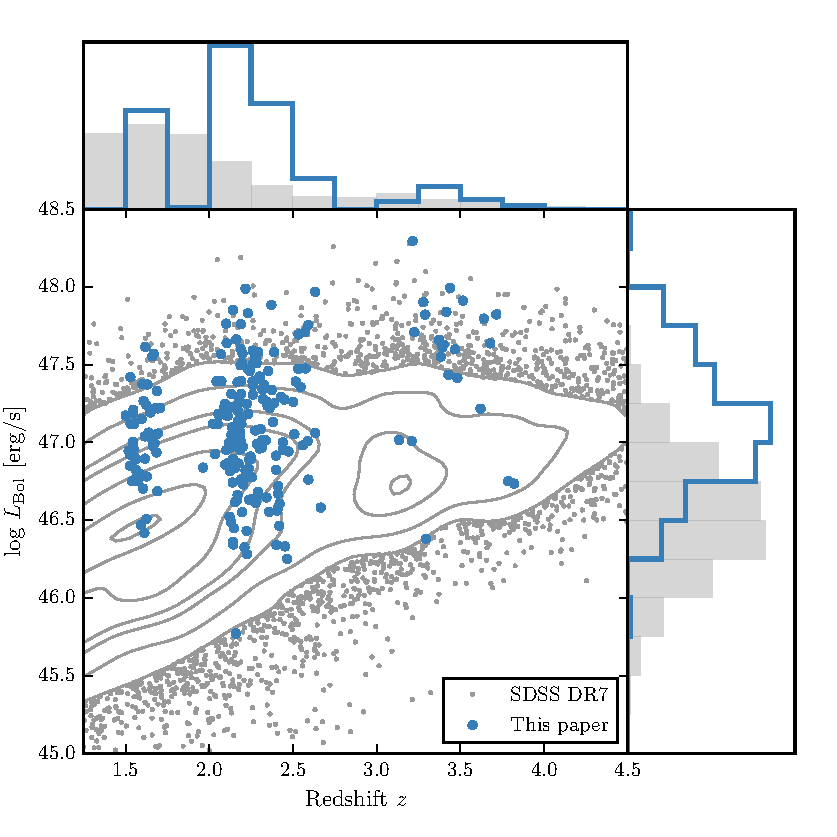
\includegraphics[width=\columnwidth]{figures/chapter03/luminosity_z.pdf} 
    \caption{The ranges in redshift and luminosity covered by our sample, relative to the redshift-luminosity distribution of the SDSS DR7 quasar catalogue. In regions of high point-density, contours show equally-spaced lines of constant probability density generated using a Gaussian kernel-density estimator. For the SDSS sample we use \citet{hewett10} redshifts and bolometric luminosities measured by \citet{shen11}. For the quasars in this paper the redshift is defined using the peak of the \hans/\hb emission and the luminosity is measured in the continuum at 1350\AA\, and converted to a bolometric quantity using the same conversion factor employed by \citet{shen11}.}     
    \label{fig:lzplane}
\end{figure}


\begin{table*}
  \centering
  \caption{The numbers of quasars with reliable \ha and \hb line measurements, the spectrographs and telescopes used to obtain the near-infrared spectra, and the instrumental configurations.}
  \label{tab:specnums}
  \begin{minipage}{16cm}
  \centering
    \begin{tabular}{cccccccc} 
    \hline
    Spectrograph & Telescope & Resolving power & Wavelength coverage & Slit width & Exposure times & \ha Sample & \hb Sample \\
    & & $\lambda/\Delta\lambda$ & $\mu$m & arcsec & hr & & \\  
    \hline
    FIRE       & MAGELLAN & 6000      & 0.80-2.50 & 0.6       & 0.5-1.0    & 18 & 19 \\
    GNIRS      & GEMINI-N & 5400      & 0.85-2.50 & 0.3-0.45 & 0.3-1.3  & 22 & 17 \\
    ISAAC      & VLT      & 5100      & 1.40-1.82 & 0.6       & 0.6-1.3  & 0  & 4 \\
    LIRIS      & WHT      & 945       & 1.39-2.42 & 1.0         & 0.2-0.8  & 15 & 0 \\
    NIRI       & GEMINI-N & 520-825   & 1.43-1.96 & 0.47-0.75 & 0.5-2.7 & 0  & 12 \\
    SINFONI    & VLT      & 2000-3000 & 1.10-2.45\footnote{$J$, $H$ or $K$ filters were employed to ensure coverage of the \hbns/[\ion{O}{III}] spectral region.} &  & 0.1-0.7  & 2  & 25 \\
    SOFI       & NTT      & 1000-2000 & 1.53-2.52\footnote{Both the low resolution red grism and the medium resolution grism, with $K$ and $H$ filters, were employed.} & 0.6       & 0.5-1.8  & 47 & 23 \\
    TRIPLESPEC & ARC-3.5m & 2500-3500 & 0.95-2.46 & 1.1-1.5   & 1.0-1.5    & 33 & 20 \\
    TRIPLESPEC & P200     & 2500-2700 & 1.00-2.40   & 1.0         &          & 23 & 19 \\
    XSHOOTER   & VLT      & 4350-7450 & 0.30-2.50   & 0.5-1.6   &     0.2-0.8     & 4  & 7 \\
    \hline
    \multicolumn{6}{c}{Total} & 164 & 144 \\
    \hline
    \end{tabular}
    \end{minipage}
\end{table*}


\subsection{Near-infrared observations}

\subsubsection{Coatman et al. (2016) Quasars}
\label{ss:paperI}

\citet{coatman16} (hereafter Paper I) observed objects drawn from the SDSS DR7 quasar catalogue.
Quasars were selected to i) have redshifts $2.14 < z < 2.51$, ii) be radio-quiet, iii) show no evidence of broad absorption lines (BALs) affecting the \ion{C}{IV} emission line, iv) be free from significant dust extinction and v) possess \ion{C}{IV}-emission shapes spanning the full range in the population.
Near-infrared spectra, including the \ha line, were obtained with the Long-slit Intermediate Resolution Infrared Spectrograph \citep[LIRIS;][]{manchado98} mounted on the 4.2\,m William Herschel Telescope (WHT) at the Observatorio del Roque de los Muchachos (La Palma, Spain).
The spectra were reduced using standard \textsc{IRAF}\footnote{IRAF is distributed by the National Optical Astronomy Observatory, which is operated by the Association of Universities for Research in Astronomy (AURA) under a cooperative agreement with the National Science Foundation.} packages, as described in Paper I. 
We have selected 15 quasars with the highest S/N \ha spectra from the original sample of 19 (see Section~\ref{sec:flagged_spectra}) and the observational properties of these quasars are summarised in Table~\ref{tab:wht}. 

\subsubsection{Shen \& Liu (2012) and Shen (2016) Quasars}

\citet{shen16a} and \citet{shen12} obtained near-infrared spectroscopy for a sample of 74 luminous, $1.5 < z < 3.5$ quasars selected from the SDSS DR7 quasar catalogue. 
Targets had to possess good optical spectra covering the \ion{C}{IV} line and have redshifts $z\sim$ 1.5, 2.1, and 3.3 to ensure that the \hbns-[\ion{O}{iii}] region was covered in one of the near-infrared $JHK$ bands.
Thirty-eight of the quasars were observed with TripleSpec \citep{wilson04} on the Astrophysics Research Consortium (ARC) 3.5\,m telescope, and 36 with the Folded-port InfraRed Echellette \citep[FIRE;][]{simcoe10} on the 6.5\,m Magellan-Baade telescope.
The reduction of the spectra is described in \citet{shen16a} and \citet{shen12}. 
The 57 quasars for which we were able to measure reliable emission line properties (Section~\ref{sec:flagged_spectra}) are summarised in Table~\ref{tab:shen}.

\subsubsection{Quasar Pairs}

Twenty per cent of our catalogue was observed as part of an ongoing effort to identify quasar pairs at very close projected separations \citep[Quasars Probing Quasars\footnote{www.ucolick.org/\textasciitilde xavier/QPQ/Quasars\_Probing\_Quasars} (QPQ);][]{hennawi06a,hennawi10}. 
The primary science driver of this work is to study the circum-galactic medium of the foreground quasars in absorption \citep{hennawi06b}.
Very accurate systemic redshift measurements are a requirement and a large amount of effort has gone into obtaining near-infrared spectra which cover low-ionisation broad lines or features from the quasar narrow line region \citep{prochaska09,lau15,hennawi15}. 
From the QPQ data set we identified 46 quasars with good-quality near-infrared spectra covering the \ha and/or \hb lines and SDSS and/or BOSS spectra covering the \ion{C}{IV} line. 
Twenty-two quasars were observed with the Gemini Near-Infrared Spectrograph \citep[GNIRS;][]{elias06} on the 8.1 m Gemini North telescope, 4 using the Infrared Spectrometer And Array Camera \citep[ISAAC;][]{moorwood98b} on the European Southern Observatory (ESO) Very Large Telescope (VLT), 11 with the Near InfraRed Imager and Spectrometer \citep[NIRI;][]{hodapp03} also on Gemini North and 9 with XSHOOTER \citep{vernet11}, again, on the VLT. 
The broad wavelength coverage of XSHOOTER means that the spectra cover the region from \ion{C}{IV} to \ha at the redshifts targeted. 
The XSHOOTER spectra have higher S/N and resolution than the SDSS/BOSS spectra in the rest-frame ultraviolet and therefore the XSHOOTER spectra are used by default to measure the \ion{C}{IV} emission. 

The  XSHOOTER  spectra  were  reduced  with  a  custom  software  package  developed  by  George  Becker \citep[for details, see][]{lau15}. 
The remaining data was processed with algorithms in the LowRedux\footnote{www.ucolick.org/\textasciitilde xavier/LowRedux} package \citep[see][]{prochaska09}.

The 46 quasars for which we were able to measure reliable emission line properties are summarised in Table~\ref{tab:qpq}.

\subsubsection{VLT SINFONI Quasars}

We performed a search of the ESO archive for high-$z$ quasars observed with the SINFONI  integral  field  spectrograph \citep{eisenhauer03,bonnet04} at VLT/UT4.
We found 37 quasars with redshifts $1.5 < z < 3.7$ which have $H$ and/or $K$ SINFONI spectroscopy, covering the \hb and \ha lines respectively, where good optical spectroscopy covering \ion{C}{IV} is also available. 
Thirty of the quasars are from a large programme led by L. Wisotzki (programme 083.B-0456(A)) to study the mass function and Eddington ratios of active BHs at redshifts $z\sim 2$ drawn from the Hamburg/ESO survey \citep{wisotzki00}.
The Hamburg/ESO optical spectra have a typical $\sim$400\kms\, spectral resolution and S/N $\gtrsim$ 10 per pixel. 
A further seven SINFONI spectra are from a programme led by  J. D. Kurk (programme 090.B-0674(B)) to obtain reliable BH mass estimates from \hans/\hb for a sample of radio-loud/radio-quiet SDSS quasars.

The SINFONI spectra were reduced using the package EASYSINF\footnote{www.mrao.cam.ac.uk/\textasciitilde rw480/easysinf}.  
The package, which is based on the ESO-SINFONI pipeline, is described in \citet{williams16}. 

The 25 quasars for which we were able to measure reliable emission line properties are summarised in Table~\ref{tab:sinf}. 

\subsubsection{ESO NTT SOFI Quasars}

Twelve per cent of the quasar catalogue derives from a large programme (programme 187.A-0645; PI: J. Hennawi) to combine near-infrared spectra from SOFI \citep{moorwood98a} on the 3.6\,m New Technology Telescope (NTT) with archival high-resolution optical spectra from the UV-Visual Echelle Spectrograph \citep[UVES;][]{dekker00} at VLT/UT2 and the High Resolution Echelle Spectrometer \citep[HIRES;][]{vogt94} at Keck to construct a legacy database of bright, high-redshift ($2 < z < 4$) quasars with both rest-frame optical spectra, covering the \hbns-[\ion{O}{III}] complex, and high-resolution rest-frame ultraviolet spectra.
The main science goal is to obtain precise systemic redshifts which are crucial for the study of absorption line systems.  
The SOFI spectra were reduced using a custom data reduction pipeline using algorithms in the LowRedux package.

Eighteen quasars have been targeted as part of the SDSS/BOSS spectroscopic quasar surveys.
In addition, 13 reduced and fluxed UVES spectra have been made available to us by A. Dall'Aglio (a description of the reduction procedure is contained in \citet{dallaglio08}).
The sample is larger ($\sim$100 quasars) but reduced UVES spectra providing rest-frame ultra-violet coverage of \ion{C}{IV} are not yet available for the remainder. 
The spectral resolution of the UVES observations is very high ($R$$\sim$40\,000) and the S/N of the spectra re-binned to a resolution of $\simeq$2000 is S/N$\simeq$300. 
The 28 quasars for which we were able to measure reliable emission line properties are summarised in Table~\ref{tab:sofijh}.

Over five nights from 2015 August 31 to September 4 we obtained near-infrared SOFI spectra for a further 26 quasars (programme 095.B-0644(A); PI: L. Coatman). 
These quasars were selected from the SDSS DR7 quasar catalogue using criteria very similar to those described in Paper I (see Section~\ref{ss:paperI}). 
In particular, we selected quasars with large \ion{C}{IV} blueshifts to improve the statistics in this region of the \ion{C}{IV} emission-line parameter space. 
The 27 quasars for which we were able to measure reliable emission line properties are summarised in Table~\ref{tab:sofilc}.

\subsubsection{P200 TripleSpec Quasars}

A further 36 quasars in our catalogue are bright SDSS quasars which were observed with the TRIPLESPEC spectrograph on the Palomar 200-inch Hale telescope (P200). 
The objects were observed with the same science goals as the SOFI NTT large programme. 
The spectra were reduced using a custom pipeline, again using algorithms in the LowRedux package. 
The 32 quasars for which we were able to measure reliable emission line properties are summarised in Table~\ref{tab:triple}.

\subsection{Optical observations}

In the previous sections, we described the infrared spectra of the 230 quasars making up our full spectroscopic catalogue. 
We will now describe the companion optical spectra, which provide coverage of the \ion{C}{IV} emission. 

Optical SDSS DR7 spectra are employed for 70 quasars in the full catalogue.  
The SDSS DR7 spectra are moderate resolution ($R$$\simeq$2000) and S/N (S/N$\simeq$20) and cover the observed-frame wavelength interval $\sim3800-9180$\,\AA.
Many of the quasars in the SDSS DR7 catalogue have been re-observed as part of the Sloan Digital Sky Survey-III: Baryon Oscillation Spectroscopic Survey \citep[SDSS-III/BOSS;][]{dawson13}. 
As the BOSS-spectra typically have higher S/N than the SDSS DR7 spectra, we have used the BOSS spectra when available (126 quasars).  
We also use high-resolution optical spectra taken with VLT/UVES (11 quasars) and VLT/XSHOOTER (8 quasars), and Hamburg/ESO spectra for a further 15 quasars.  

In summary, we have assembled a sample of 230 luminous, high-$z$ quasars with optical and near-infrared spectra.
This will allow us to directly compare virial BH mass estimates based on the \ion{C}{IV} line-width with estimates based on the line-widths of the low-ionisation Balmer lines \ha and \hbns.  

\section{Spectral Measurements}

Conventionally, single-epoch virial estimates of the BH mass are a function of the line-of-sight velocity width of a broad emission line and the quasar luminosity. 
The velocity width is a proxy for the virial velocity in the broad line region (BLR) and, as revealed in reverberation-mapping studies, the luminosity is a proxy for the typical size of the BLR \citep[the $R-L$ relation; e.g.][]{kaspi00,kaspi07}. 
Most reverberation mapping campaigns have employed \hb time-lags and velocity widths, but the line-widths of \ha and \ion{Mg}{II}$\lambda$2800 have been shown to yield consistent BH masses \citep[e.g.][]{mclure02,greene05,onken08,shen08,wang09,rafiee11,mejia-restrepo16}. 
In Section~\ref{sec:hahbcomparison} we verify that this is the case for the 99 quasars in our sample with measurements of both \ha and \hb lines.     

At redshifts $z> 2.2$, where the hydrogen Balmer lines and \ion{Mg}{II} are no longer accessible in many optical spectra, the \ion{C}{IV}$\lambda$1550 emission doublet has routinely been used to provide estimates of the virial velocity \citep[e.g.][]{shen11}. 
As has long been recognised \citep{gaskell82, tytler92} the \ion{C}{IV} emission line in many quasars includes contributions from gas that does not straightforwardly relate to virial motions within a stable BLR.
A number of studies \citep[e.g.][]{shen08, richards11} have shown that the amplitude of the systematic shift of the \ion{C}{IV} emission to shorter wavelengths (relative to the systemic velocity) is strongly correlated with the properties of the emission-lines and the overall spectral energy distributions (SEDs). 

In our work, a robust measure of the \ion{C}{IV} emission-line `blueshift' provides the basis for the corrected \ion{C}{IV} velocity-width measurements, and hence BH masses.
The effectiveness of the scheme is validated via a direct comparison of the \ion{C}{IV} velocity-widths to the Balmer emission velocity-widths in the same quasars. 
Our process is as follows. 
First, an accurate measure of the quasar's systemic redshift is required, for which we adopt the centre of the Balmer emission, where the centre, $\lambda_{\rm half}$, is the wavelength that bisects the cumulative total flux. 
Balmer emission centroids are available for all quasars in the catalogue but we verify that the measure is relatively unbiased through a comparison of the centroids to the wavelengths of the peak of the narrow [\ion{O}{III}]\ll4960,5008 doublet for the subset of spectra where both are available. 
Second, the blueshift of the \ion{C}{IV} emission line is determined. 
Again, we adopt the line centroid to provide a robust measure of the \ion{C}{IV} emission blueshift.
The blueshift (in \kms) is defined as $c\times$(1549.48-$\lambda_{half}$)/1549.48 where $c$ is the velocity of light and 1549.48\,\AA \ is the rest-frame wavelength for the \ion{C}{IV} doublet, assuming equal contribution from both components.
Positive blueshift values indicate an excess of emitting material moving towards the observer and hence out-flowing from the quasar. 

Emission-line velocity widths are derived from the full-width-at-half-maximum (FWHM) of the lines but we also compute the line dispersion (calculated from the flux-weighted second moment of the velocity distribution) as some authors have claimed this provides a better estimate of the virial velocity \citep{denney13}. 

To minimise the impact of the finite S/N of the quasar spectra and the presence of absorption features superposed on the broad emission lines we first fit a parametric model to the continuum and the emission lines. 
The purpose of the parametric fits is, however, simply to provide higher S/N representations of the emission features. 
The particular form of the model parametrizations is not important and the fits are used only to provide robust line parameters, such as the centroid $\lambda_{\rm half}$, and FWHM, which are measured non-parameterically from the best-fitting model. 
The models used and the fitting procedure are described below. 
The issues involved in deriving parameters for broad emission lines from spectra of modest S/N -- for example, subtraction of narrow line emission, subtraction of \ion{Fe}{II} emission -- have been covered comprehensively by other authors \citep[e.g.][]{shen11,shen12,denney13,shen16a} and, as far as possible, we follow standard procedures described in the literature. 

\subsection{\ion{C}{IV}}
\label{sec:civ}

The parametrization of the \ion{C}{IV} emission line is identical to the one described in Paper I. 
We first define a power-law continuum, $f(\lambda) \propto \lambda^{-\alpha}$, with the slope, $\alpha$, determined using the median values of the flux in two continuum windows at 1445-1465 and 1700-1705\AA. 
The continuum emission is subtracted from the spectra, which is then transformed from wavelength units into units of velocity relative to the rest-frame line-transition wavelength for the \ion{C}{IV} doublet (1549.98\AA, assuming equal contributions from both components). 
The parametric model is ordinarily fit within the wavelength interval 1500-1600\AA\, (corresponding to approximately $\pm 10\,000$ \kms\, from the rest-frame transition wavelength), a recipe that is commonly adopted \citep[e.g.][]{denney13}. 
The line-window was extended if more than 5\,per cent of the total flux in the profile was present blueward of the short wavelength limit. 
Narrow absorption features, which are frequently found superimposed on \ion{C}{IV} emission (see, for example, the \ion{C}{IV} profile of J0942+3523 in Fig.~\ref{fig:examplegrid}), were masked out during the fit. 


The \ion{C}{IV} emission was fit with sixth-order Gauss-Hermite (GH) polynomials, using the normalisation of \citet{marel93} and the functional forms of \citet{cappellari02}. 
We allowed up to six components, but in many cases a lower order was sufficient (40 and 45 per cent were fit with second- and fourth-order GH polynomials respectively).
GH polynomials were chosen because they are flexible enough to model the often very asymmetric \ion{C}{IV} line profile. 
The flip-side of this flexibility, however, is that the model has a tendency to over-fit when spectra possess low S/N. 
The fits were therefore carefully checked visually and the number of components reduced if over-fitting was evident.

In Paper I we found that using the commonly employed three-Gaussian component model, rather than the GH polynomials, resulted in only marginal differences in the line parameters. 
Our best-fit parameters are also in good agreement with \citet{shen11}, who employ a multi-Gaussian parametrization. 
In the Appendix we demonstrate that the mean difference between our FWHM measurements and the measurements of \citet{shen11} is just 200\kms for the quasars common to both samples, which is much too small to have any significant effect on our results.

\subsection{\ha}

A power-law continuum is fit using two continuum windows at 6000-6250 and 6800-7000\,\AA. 
The continuum-subtracted flux is then fit in the wavelength interval 6400-6800\,\AA. 
We adopt a rest-frame transition wavelength of 6564.89\,\AA\, to transform wavelengths into equivalent Doppler velocities. 
The broad component of \ha is fit using one or two Gaussians, constrained to have a minimum FWHM of 1200\kms. When two Gaussians are used, the velocity centroids are constrained to be the same.

The emission-line profiles of both \hb and \ha frequently include a significant narrow component from the physically more extended narrow line region (NLR). 
Additional Gaussian components were included in our parametric model to fit the narrow component of \ha as well as [\ion{N}{II}]\ll6548,6584 and [\ion{S}{II}]\ll6717,6731.
This resulted in a better fit to the observed flux in 50\, per cent of cases. 
We impose a 1200\kms upper limit on the FWHM of all narrow lines and the amplitudes of all components must be non-negative.
The relative flux ratio of the two [\ion{N}{II}] components is also fixed at the expected value of 2.96.
In 70\, per cent of the spectra the [\ion{O}{III}]\ll4960,5008 doublet is detected at moderate S/N in the \hb region. 
In these cases the peak of the [\ion{O}{III}] is used to fix the velocity offsets and the FWHMs of the narrow line components in the \ha region.  
For spectra where the [\ion{O}{III}] doublet does not constrain the velocity and FWHM accurately, the narrow emission in the \ha and \hb regions are fitted independently but, for each region, the individual narrow-line velocity offsets and the FWHMs are constrained to be identical. 
In these objects the narrow line contribution is generally weak, and so does not have a large effect on the line parameters we measure for the broad component.   

The model described above is very similar to the one described in \citet{shen16a}, \citet{shen12} and \citet{shen11}, the only major difference being that we do not fit the \ha and \hb emission regions simultaneously. 
In Appendix~\ref{appendix:shen}, we compare our \ha line measurements for the subset of our sample taken from \citet{shen16a} and \citet{shen12}, and find a scatter of just 0.07 dex. 

\subsection{\hb and [\ion{O}{III}]}

Emission from optical \ion{Fe}{II} is generally strong in the vicinity of \hbns.
We therefore fit a combination of a power-law continuum and an optical \ion{Fe}{II} template -- taken from \citet{boroson92} -- to two windows at 4435-4700 and 5100-5535\,\AA. 
The \ion{Fe}{II} template is convolved with a Gaussian, and the width of this Gaussian, along with the normalisation and velocity offset of the \ion{Fe}{II} template, are free variables in the pseudo-continuum fit.
We use the same model to fit the broad and narrow components of \hb as was used with \hans. 
Each line in the [\ion{O}{III}] doublet is fit with two Gaussians, to model both the systemic and any outflow contributions. 
The peak flux ratio of the [\ion{O}{III}] 4960\,\AA\, and 5008\AA\, lines is fixed at 1:3. 
As for the fit to the narrow lines in the spectral region around \hans, the width and velocity offsets of all the narrow components are set to be equal, and an upper limit of 1200\kms is placed on the FWHM. 

\subsection{Fitting procedure}

Model parameters were derived using a standard variance-weighted least-squares minimisation procedure employing the Levenberg-Marquardt algorithm. 
Prior to the fit, the spectra were inspected visually and regions significantly affected by absorption or of low S/N were masked out.

In Fig.~\ref{fig:examplegrid} we present our parametric fits to the \ion{C}{IV}, \ha and \hb emission lines in a handful of quasars, which have been chosen to illustrate the range of spectrum S/N and line shapes in the sample.  
The mean reduced chi-squared values in our \hans, \hb and \ion{C}{IV} fits are 1.69, 1.62, and 1.77 respectively and, in general, there are no strong features observable in the spectrum minus model residuals. 
Table~\ref{tab:specmeasure} includes the line parameters of our best-fitting model for each line.
The reported line-width measures are corrected for instrumental broadening by subtracting the resolution of the spectrograph in quadrature. 
The spectrograph resolutions, which we estimate from the line widths in the observed sky spectra, range from 25\kms\, for XSHOOTER to 477\kms\, for the low-resolution LIRIS grism and are therefore small relative to the quasar broad line widths.

\begin{table*}
  \centering
  \vspace*{-0.4cm}
  \caption{The format of the table containing the emission line properties from our parametric model fits. The table is available in machine-readable form in the online journal.}
  \label{tab:specmeasure}
  \vspace*{-0.1cm}
  \begin{minipage}{16cm}
  \centering
    \begin{tabular}{ccc} 
    \hline
    & Units & Description \\ 
    \hline
    NAME & & Catalogue name \\
    FWHM\_BROAD\_HA & \kms & FWHM of broad \ha line \\ 
    FWHM\_BROAD\_HA\_ERR & \kms & \\
    SIGMA\_BROAD\_HA & \kms & Dispersion of broad \ha line\\
    SIGMA\_BROAD\_HA\_ERR & \kms & \\
    Z\_BROAD\_HA & & Redshift from broad \ha line\\
    FWHM\_BROAD\_HB & \kms & FWHM of broad \hb line \\
    FWHM\_BROAD\_HB\_ERR & \kms & \\
    SIGMA\_BROAD\_HB & \kms & Dispersion of broad \hb line \\
    SIGMA\_BROAD\_HB\_ERR & \kms & \\
    Z\_BROAD\_HB & & Redshift from broad \hb line\\
    FWHM\_CIV & \kms & FWHM of \ion{C}{IV} doublet \\
    FWHM\_CIV\_ERR & \kms & \\
    SIGMA\_CIV & \kms & Dispersion of \ion{C}{IV} doublet \\
    SIGMA\_CIV\_ERR & \kms & \\
    BLUESHIFT\_CIV\_HA & \kms & Blueshift of \ion{C}{IV} relative to centroid of broad \hans \\
    BLUESHIFT\_CIV\_HA\_ERR & \kms & \\
    BLUESHIFT\_CIV\_HB & \kms & Blueshift of \ion{C}{IV} relative to centroid of broad \hbns \\
    BLUESHIFT\_CIV\_HB\_ERR & \kms & \\
    LOGL5100 & \ergs & Monochromatic continuum luminosity at 5100\AA \\
    LOGL1350 & \ergs & Monochromatic continuum luminosity at 1350\AA\\
    \hline
    \end{tabular}
  \vspace*{-0.4cm}
  \end{minipage}
\end{table*}

\begin{figure*}
    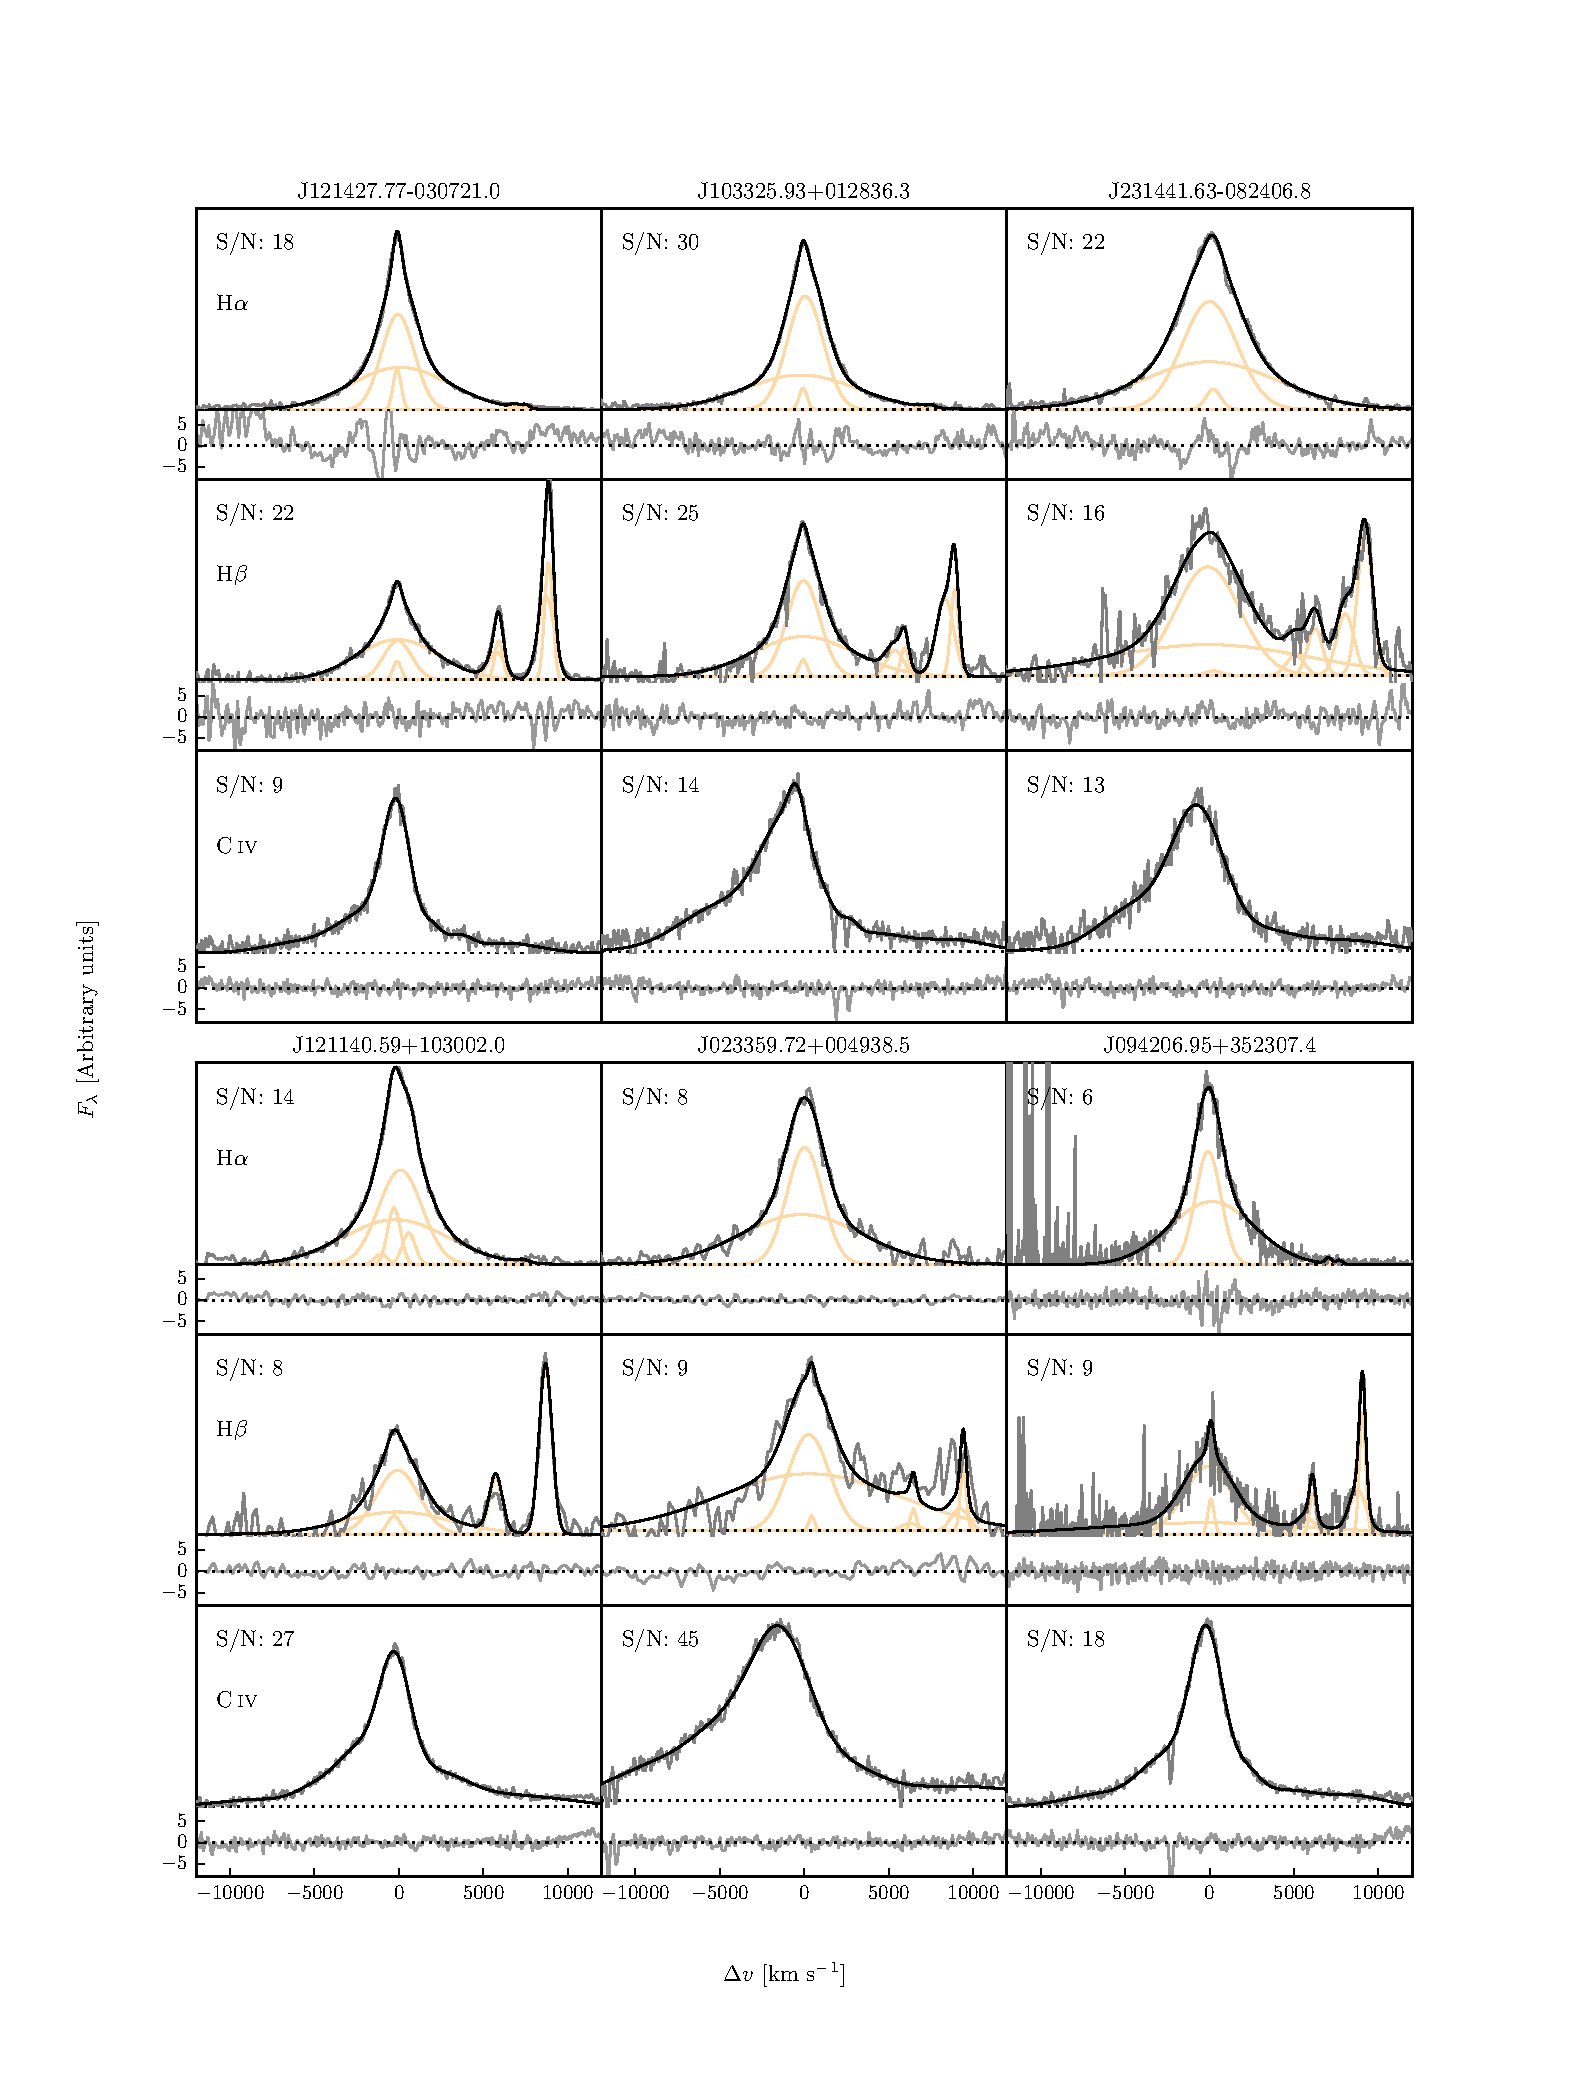
\includegraphics[width=2\columnwidth]{figures/chapter03/example_grid.pdf} 
    \caption{Model fits to continuum-subtracted \hans, \hbns, and \ion{C}{IV} emission in six quasars, chosen to represent the range of S/N (indicated in the figure and given per 150\kms\, pixel in the continuum) and line shapes present in the catalogue. The data is shown in grey, the best-fitting parametric model in black, and the individual model components in orange. The centroid of the broad \ha emission is used to set the redshift, and $\Delta{v}$ is the velocity shift from the line rest-frame transition wavelength. Below each fit we plot the data minus model residuals, scaled by the errors on the fluxes.} 
    \label{fig:examplegrid}
\end{figure*}


\subsection{Spectra removed from sample}
\label{sec:flagged_spectra}

\begin{table}
  \centering
  \caption{The number of spectra removed from our sample by the cuts described in Section~\ref{sec:flagged_spectra}.}
  \label{tab:flagged_spectra}
    \begin{tabular}{cccc}
    \hline
    & & \ha sample & \hb sample \\ 
    \hline
    \multicolumn{2}{c}{Total} & 194 & 279 \\
    \hline
    \hans/\hbns & Wavelength & 6 & 27 \\
    & S/N & 8 & 83 \\
    \hline
    \ion{C}{IV} & Wavelength & 6 & 5 \\
    & S/N & 4 & 12 \\
    & Absorption & 6 & 8 \\
    \hline
    \multicolumn{2}{c}{Total remaining} & 164 & 144 \\
    \hline
    \end{tabular}
\end{table}


Through visual inspection we flagged and discarded the spectra of quasars for which reliable emission line parameters could not be obtained.

First, we flagged emission lines in spectra that possessed insufficient S/N. 
A single minimum S/N threshold was not entirely effective and, instead, spectra were flagged when it was judged conservatively that no meaningful constraints could be placed on the velocity centroid and/or width of the emission-line. 

Second, we flagged emission lines where significant regions of the continuum and/or emission line fell outside of the wavelength coverage of the spectra. 
Reliable continuum definition and subtraction is not straightforward for emission lines so affected. 

Third, we flagged \ion{C}{IV} emission lines because of strong, narrow absorption close to the peak of the line where reliable interpolation across the absorption, using our parametric model, was not possible. 

The number of spectra that are removed by each cut is given in Table~\ref{tab:flagged_spectra} and the distribution in redshift and luminosity is shown in Fig.~\ref{fig:flagged_spectra}. 
Unsurprisingly, there is a preferential removal of intrinsically faint quasars, whose spectra can be of poorer S/N, and a loss of quasars at redshifts $z\sim2.6$ where the \ha emission falls at the edge of the $K$-band.
\hb is much weaker than \hans, and the \hb spectra are generally of lower S/N. 
As a result, the fraction of \hb spectra that are flagged -- 39 per cent -- is particularly high.   

\begin{figure}
    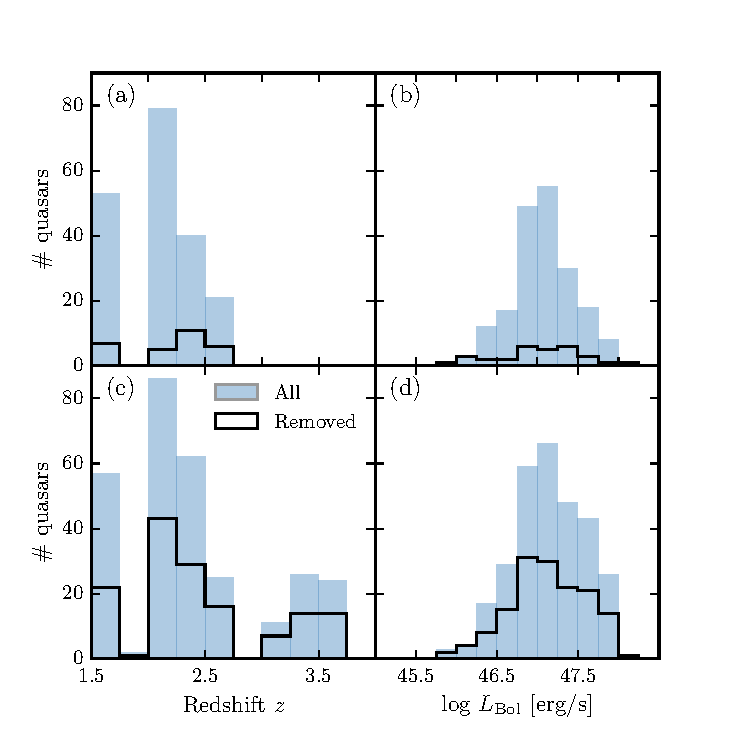
\includegraphics[width=\columnwidth]{figures/chapter03/flagged_spectra.pdf} 
    \caption{The redshift and luminosity distributions of the spectra removed from our \hans/\ion{C}{IV} (a, b) and \hbns/\ion{C}{IV} (c, d) samples.} 
    \label{fig:flagged_spectra}
\end{figure}

\subsection{Emission-line parameter uncertainties}

The 1$\sigma$ error bars calculated from the covariance matrix in least-squares minimisation will underestimate the true uncertainties on the line parameters, since they do not account for systematic errors such as the significant uncertainty introduced in the continuum subtraction procedure.  
To calculate more realistic uncertainties on our fitted variables we employed a Monte Carlo approach. 
One thousand artificial spectra were synthesised, with the flux at each wavelength drawn from a Normal distribution (mean equal to the measured flux and standard deviation equal to the known error).
Our emission-line fitting recipe was then implemented on each of these mock spectra. 
The uncertainty in each parameter is given by the spread in the best-fitting values from the one thousand realisations of the fitting routine. 
In some cases the standard deviation of the parameter distribution was biased by extreme values caused by bad fits\footnote{In the analysis of the real spectra such fits are identified via visual inspection.}. 
We therefore chose to measure the spread in the parameter distribution by fitting a composite model with two Gaussian components -- one to model uncertainty in the parameter and the other any possible outlier component. 
The uncertainty in each line parameter was then taken to be the width of the narrower Gaussian. 

\subsection{Contemporaneity of spectra}

The epochs of the near-infrared and optical spectra can differ by many years.
For example, the NTT SOFI spectra were taken $\sim$14 years after the SDSS spectra, and the VLT SINFONI spectra 20 years or more after the Hamburg/ESO observations\footnote{Time differences in the quasar rest-frame are reduced by a factor of ($1 + z$).}.
If the broad emission line profiles varied significantly on these time-scales the relation between the \ion{C}{IV} and Balmer line-width measurements could be blurred. 

Cases do exist of dramatic changes in quasar spectra over short time-scales, but this phenomenon is rare \citep{macleod16}. 
In our spectroscopic catalogue there are 112 SDSS DR7 quasars which are re-observed in BOSS and included in the DR12 quasar catalogue. 
The mean time elapsed between the two sets of observations is $\sim$8 years. 
The root-mean-square difference in the \ion{C}{IV} FWHM measured from the BOSS and SDSS spectra is a modest $\simeq$500\kms. 
Differences in the S/N of the spectra will make a substantial contribution and the scatter due to true variations in the \ion{C}{IV} velocity-width will be significantly smaller than 500\kms. 
We conclude therefore that any intrinsic changes with time do not materially affect the emission line measurements.

\subsection{Quasar monochromatic luminosity}

Computing virial BH masses also requires the quasar luminosity in an emission-line free region of the continuum adjacent to the broad line being used. 
The luminosity is used as a proxy for the size of the BLR. 
The monochromatic continuum flux is generally measured at 1350\,\AA\ for \ion{C}{IV} and 5100\,\AA\, for \ha and \hbns. 

Relative flux-calibration of the infrared spectra as a function of wavelength has been achieved, to $\simeq$10 per cent, through observations of appropriate flux standards. 
The absolute flux levels, however, can be in error by large factors due to variable atmospheric conditions combined with the narrow slit widths. 
For the majority of the quasars we have, therefore, established the absolute flux scale for each near-infrared spectrum using the same quasar SED-model fitting scheme employed in Paper I.
The SED model, described in \citet{maddox12}, gives a very good fit to the SDSS and UKIDSS magnitudes of SDSS DR7 quasars, reproducing the individual magnitudes with a $\sigma <$0.1\,mag. 
For 207 quasars, ($Y$)$JHK$ passband magnitudes from the UKIRT Infrared Deep Sky Survey \citep[UKIDSS;][]{lawrence07} Large Area Survey, the Two Micron All Sky Survey \citep[2MASS;][]{skrutskie06} and the Visible and Infrared Survey Telescope for Astronomy (VISTA) Hemisphere Survey \citep[VHS;][]{mcmahon13} and Kilo-Degree Infrared Galaxy \citep[VIKING;][]{edge13} survey are available. 
The SED model was fit to the infrared magnitudes; integrating the SED model through the pass-band transmission functions, to give model magnitudes, and performing a variance weighted least-squares fit to the observed magnitudes. 
The flux at 5100\,\AA\, was then taken from the normalised model.

For 19 of the remaining 23 quasars, where near-infrared photometry was not available, the quasar SED model was fit to the SDSS spectra, the flux calibration of which are known to be excellent.  
The fit was done using a simple variance-weighted chi-squared minimisation procedure in emission line-free intervals of the optical spectra.   
The model includes a reddening, $E(B-V)$, based on a Small Magellanic Cloud-like extinction curve, and an overall normalisation of the model as free parameters.
In practice, the quasars possess only very modest reddenings, with $E(B-V)\simeq$0.0-0.1.
The flux at 5100\,\AA\, was then, again, taken from the normalised SED model.
For the four remaining quasars, which possess neither near-infrared photometry nor SDSS DR7 spectra, we fit the SED model to the BOSS DR12 spectra. 
To avoid the known issues in the flux calibration of the BOSS DR12 quasar spectra at observed-frame blue wavelengths \citep{lee13}, our fitting was confined to rest-frame wavelengths long-ward of 1275\AA. 

Comparison of the 5100\,\AA\, luminosity, computed using the photometry- and spectrum-based methods for 177 quasars, showed a scatter of just $\sim$0.1\,dex.
We therefore assume 0.1\,dex to be the measurement uncertainty on the 5100\,\AA\, luminosities. 

For 34 quasars in the catalogue the optical spectra come from surveys other than SDSS/BOSS and optical magnitudes from recent epochs are not available. 
In order to obtain an estimate of the luminosity at 1350\,\AA\, for the 30 quasars, we take the standard \citet{maddox12} quasar SED model, normalised to the near-infrared magnitudes, and read off the flux at 1350\,\AA. 

For all the catalogue quasars, the optical and near-infrared spectra as well as the near-infrared photometry were obtained at different epochs, with rest-frame time differences of up to $\sim$5\,years. 
Intrinsic quasar photometric variability in the rest-frame ultraviolet and optical will therefore add additional scatter of $\sim$0.2\,mag \citep[e.g.][]{macleod10} to the derived 1350- and 5100\,\AA-luminosities. 

Given that the luminosity enters into the calculation of BH-mass only as the square-root, the uncertainty on the luminosities does not make a large contribution to the uncertainties in the BH mass estimates.  

\section{An empirical correction to \ion{C}{IV}-based virial BH-mass estimates}

\subsection{\hans/\hb FWHM comparison}
\label{sec:hahbcomparison}

BH-mass calibrations which use the width of the broad \hb emission line as a proxy for the virial velocity are widely regarded as the most reliable, since most reverberation mapping employs the \hb line and the $R-L$ relation has been established using \hbns.
When \hb is not available, \ha has been shown to be a reliable substitute \citep[e.g.][]{greene05,shen11,shen12}. 

\begin{figure}
    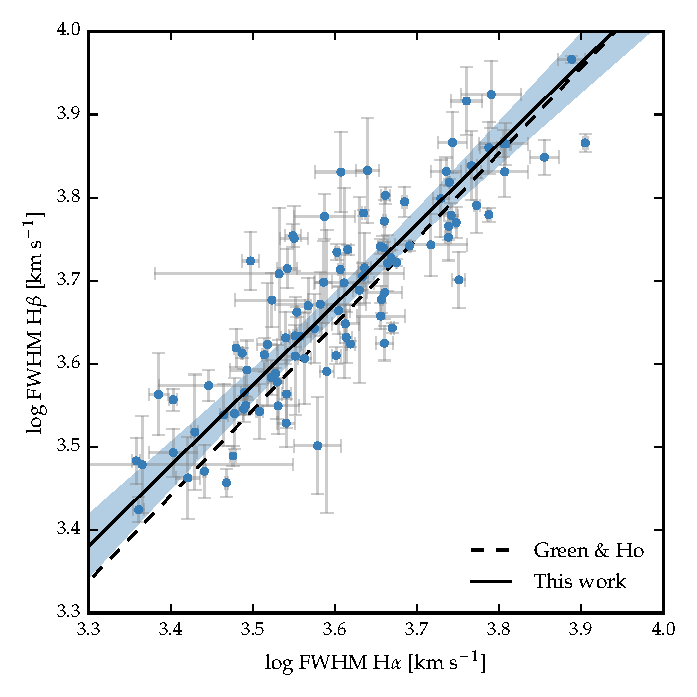
\includegraphics[width=\columnwidth]{figures/chapter03/ha_hb_width_comparison.pdf} 
    \caption{Comparison of \ha and \hb FWHM measurements for 99 quasars. The solid line is our best-fitting power-law model, and the blue-shaded region shows the 2-$\sigma$ uncertainties on the model parameters. The dashed line is the relation found by \citet{greene05} using a sample of $z<0.35$ SDSS AGN.} 
    \label{fig:hahbcomp}
\end{figure}

In our sample, we have 99 quasars with reliable measurements of both \ha and \hb lines. 
The 99 objects include 21 quasars which were excluded from the main 308-object catalogue because adequate measurements of the \ion{C}{IV} FWHM and blueshift could not be acquired. 
The line widths are compared in Fig.~\ref{fig:hahbcomp} and, as expected, a tight correlation is observed.  
\citet{greene05}, using a sample of 162 quasars with high S/N SDSS spectra at $z < 0.35$, established the following relation between the \ha and \hb FWHMs

\begin{equation}
  \rm{FWHM}(\rm{H}\beta) = \left( 1.07 \pm 0.07 \right) \times 10^3 \left( \frac{ \rm{FWHM}(\rm{H}\alpha) }{10^3 ~\rm{km}~\rm{s}^{-1} } \right)^{(1.03 \pm 0.03)}
\end{equation}

The relation is shown as the dashed line in Fig.~\ref{fig:hahbcomp}.
The root-mean-square scatter about this relation is 0.07\,dex, compared to the $\sim$0.1\,dex found by \citet{greene05}. 
However, we find a systematic offset, in the sense that the \hb line-widths we measure are on average larger by 270\kms\, than predicted by the \citet{greene05} relation. 
As our sample covers higher redshifts and luminosities than the sample in \citet{greene05}, we derive a new relation between the \ha and \hb FWHMs.       

We assume a relation of the same form used by \citet{greene05}, i.e. a simple power-law, and infer the model parameters by fitting a linear model (with slope $\alpha$ and intercept $\beta$) in log-log space.
The fit is performed within a Bayesian framework described by \citet{hogg10}. 
Each data point is treated as being drawn from a distribution function that is a convolution of the projection of the point's covariance tensor, of variance $\Sigma_i^2$, with a Gaussian of variance $V$ representing the intrinsic variance in the data.
The log-likelihood is then given by 

\begin{equation}
  {\rm ln} {\cal L} = - \sum_{i=1}^N \frac{1}{2} {\rm ln}\left[2\pi\left(\Sigma_i^2 + V\right)\right] - \sum_{i=1}^N \frac{\Delta_i^2}{2[\Sigma_i^2 + V]} 
\end{equation}

\noindent where $\Delta_i$ is the orthogonal displacement of each data point from the linear relationship. 
An advantage of this approach is that it allows a proper treatment of the measurement errors on both variables, which in this case are comparably large.
The model also makes the reasonable assumption that there is an intrinsic scatter in the relationship between the variables that is independent of the measurement errors.  
Following the suggestion by \citet{hogg10}, the linear model was parametrized in terms of ($\theta$,~$b_\bot$), where $\theta$ is the angle the line makes with the horizontal axis and $b_\bot$ is the perpendicular distance from the line to the origin.
Uniform priors were placed on these parameters, and the Jeffreys prior (the inverse variance) was placed on the intrinsic variance. 
The posterior distribution was sampled using a Markov Chain Monte Carlo (MCMC) method using the Python package {\tt emcee} \citep{foreman13}. 
 
The one- and two-dimensional posterior distributions are shown in Fig.~\ref{fig:ha_hb_mcmc_samples}. 
The solid line in Fig.~\ref{fig:hahbcomp} is the maximum likelihood solution

\begin{equation}
  \label{eq:ha2hb}
  \rm{FWHM}(\rm{H}\beta) = \left( 1.23 \pm 0.10 \right) \times 10^3 \left( \frac{\rm{FWHM}(\rm{H}\alpha)}{10^3 {\rm km\,s^{-1}}} \right)^{0.97 \pm 0.05}
\end{equation}

\noindent and the shaded region shows the 2$\sigma$ uncertainties on the model parameters.

As discussed above, our relation is displaced to slightly higher \hb FWHM than the \citet{greene05} relation -- the offset is 210\kms\, for a quasar with \ha FWHM 4500\kms.  
We infer a power-law index that, although slightly shallower, is consistent with the \citet{greene05} index within the quoted uncertainties. 
The intrinsic scatter in the data, $\sigma_I$, we infer from  the fit is 0.04 dex. 
This is smaller than the total scatter seen in Fig.~\ref{fig:hahbcomp} (0.06 dex), which suggests that measurement errors make a significant contribution to the total scatter in the relation. 

\begin{figure}
    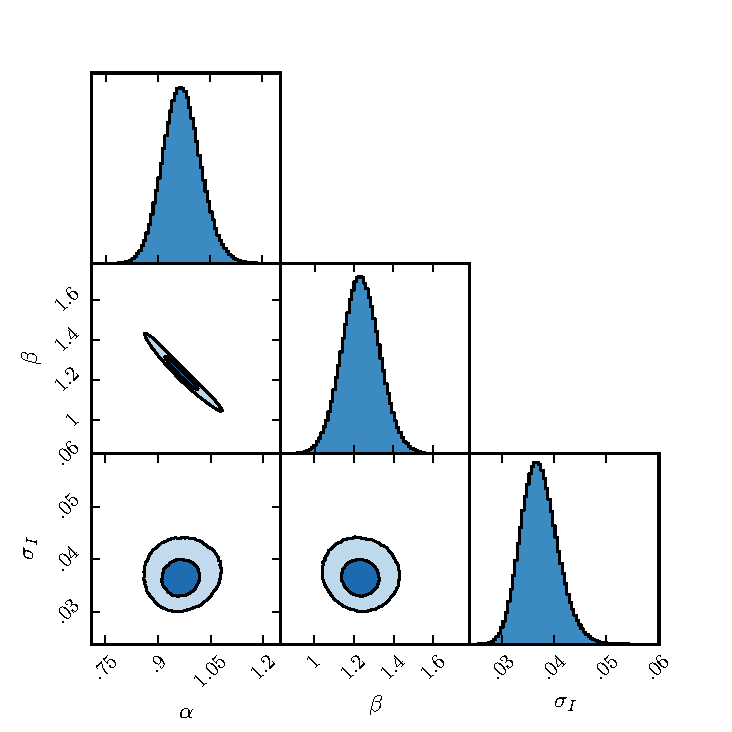
\includegraphics[width=\columnwidth]{figures/chapter03/ha_hb_mcmc_parameters.pdf} 
    \caption{One- and two-dimensional projections of the MCMC sampling of the posterior distribution from the fit in Fig.~\ref{fig:hahbcomp}. $\alpha$ is the power-law index, $10^\beta$ is the normalisation, and $\sigma_I$ is the intrinsic scatter. In the two-dimensional projections, 1- and 2-$\sigma$ contours are shown.} 
    \label{fig:ha_hb_mcmc_samples}
\end{figure}

For 19 of the 99 quasars with \hb and \ha emission profiles, one of the two Gaussians used to reproduce the \hb profiles has a FWHM greater than 20\,000\kms and a fractional contribution to the total \hb broad line flux of $>$0.3 \citep{marziani09,marziani13}.  
Such a broad component is not seen in the \ha profiles and the very broad \hbns-component may be an artifact of the fitting scheme.
A particular issue for \hb is the presence of \ion{Fe}{II} emission, often at a significant level.
Furthermore, additional lines could be contributing to the underlying continuum \citep[e.g. the \ion{He}{I}\ll4922,5017 doublet;][]{veron02,zamfir10}. 

In Sec.~\ref{sec:correction} we use the whole of the \hb profile to derive an un-biased BH mass.  
If, instead, the FWHM is calculated from the narrower of the two Gaussian components rather than the composite profile, then the \hb FWHM decreases by 630\kms on average.
The \ha FWHM, which are calibrated against the \hb FWHM, will also decrease by the same amount on average. 
This will enhance the \ion{C}{IV} FWHM relative to the \hans/\hb FHWM by $\sim$15\,per cent and increase the size of the correction which must be applied to the \ion{C}{IV}-based BH masses by $\sim$30\,per cent.  

\subsection{Measuring the quasar systemic redshift}

An accurate measure of the quasar's systemic redshift is required in order for the blueshift of the \ion{C}{IV} emission line to be determined.
Balmer emission centroids, where the centroid, $\lambda_{\rm half}$, is the wavelength that bisects the cumulative total flux, are available for all quasars in the catalogue and so we use this to define the systemic redshift.

For 83 and 120 quasars in the \ha and \hb samples respectively narrow [\ion{O}{III}] emission is also detected. 
In the model fit to the \hb region the velocity centroids of the broad \hbns-line and the core component of the [\ion{O}{III}] emission were deliberately determined separately.
We find the intrinsic difference in the velocity centroids of the Balmer broad emission and the narrow [\ion{O}{III}] emission to have a dispersion of 360\kms, which is very similar to the value found by \citet{shen16b}. 
However, the median velocity centroid of the narrow component of the [\ion{O}{III}] emission is blueshifted by 270\kms\, relative to the centroid of the broad Balmer line. 
Applying our parametric model fitting routine to the composite spectrum from \citet{hewett10}, which is constructed using relatively low redshift SDSS quasars with $L_{\rm Bol}\sim10^{44}$\,erg\,s$^{-1}$, the centroids of the broad component of \hb and the narrow component of [\ion{O}{III}] are found to be at essentially identical velocities, suggesting that the blueshifting of narrow [\ion{O}{III}] could be luminosity dependent.
Regardless, since both the systematic offset and the scatter are small in comparison to the dynamic range in \ion{C}{IV} blueshifts, the blueshift-based empirical correction we will derive does not depend on whether the broad Balmer emission or the [\ion{O}{III}] centroid is used to define the systemic redshift. 

\subsection{Balmer/\ion{C}{IV} line widths as a function of \ion{C}{IV}-blueshift}
\label{sec:correction}

In this section we directly compare the \ion{C}{IV} and \hans/\hb line widths as a function of the \ion{C}{IV} blueshift. 
Because virial BH mass estimates are generally based on the \hb FWHM, we first convert our \ha FWHM measurements to equivalent \hb FWHM using Eq.~\ref{eq:ha2hb}.  
In Fig.~\ref{fig:correction}a and b we show the \ion{C}{IV} FWHM relative to both the (\hbns-scaled) \ha FWHM and the \hb FWHM, as a function of the \ion{C}{IV} blueshift. 

Employing the same Bayesian fitting framework described in Section~\ref{sec:hahbcomparison}, we fit independent linear models to the \ion{C}{IV} FWHM relative to the \ha and \hb FWHM as a function of the \ion{C}{IV} blueshift. 
As before, our model has an additional parameter representing any intrinsic scatter in the relationship between the variables which is independent of measurement errors.  
We also tested a model where some fraction of the data points (which is free to vary) are drawn from an outlier distribution, represented by a broad Gaussian centered on the mean of the data. 
We found, however, that the inferred outlier fraction was very low (0.004, corresponding to $\sim$0.7 data points) and so did not include such a component in our model. 

\begin{figure*}
    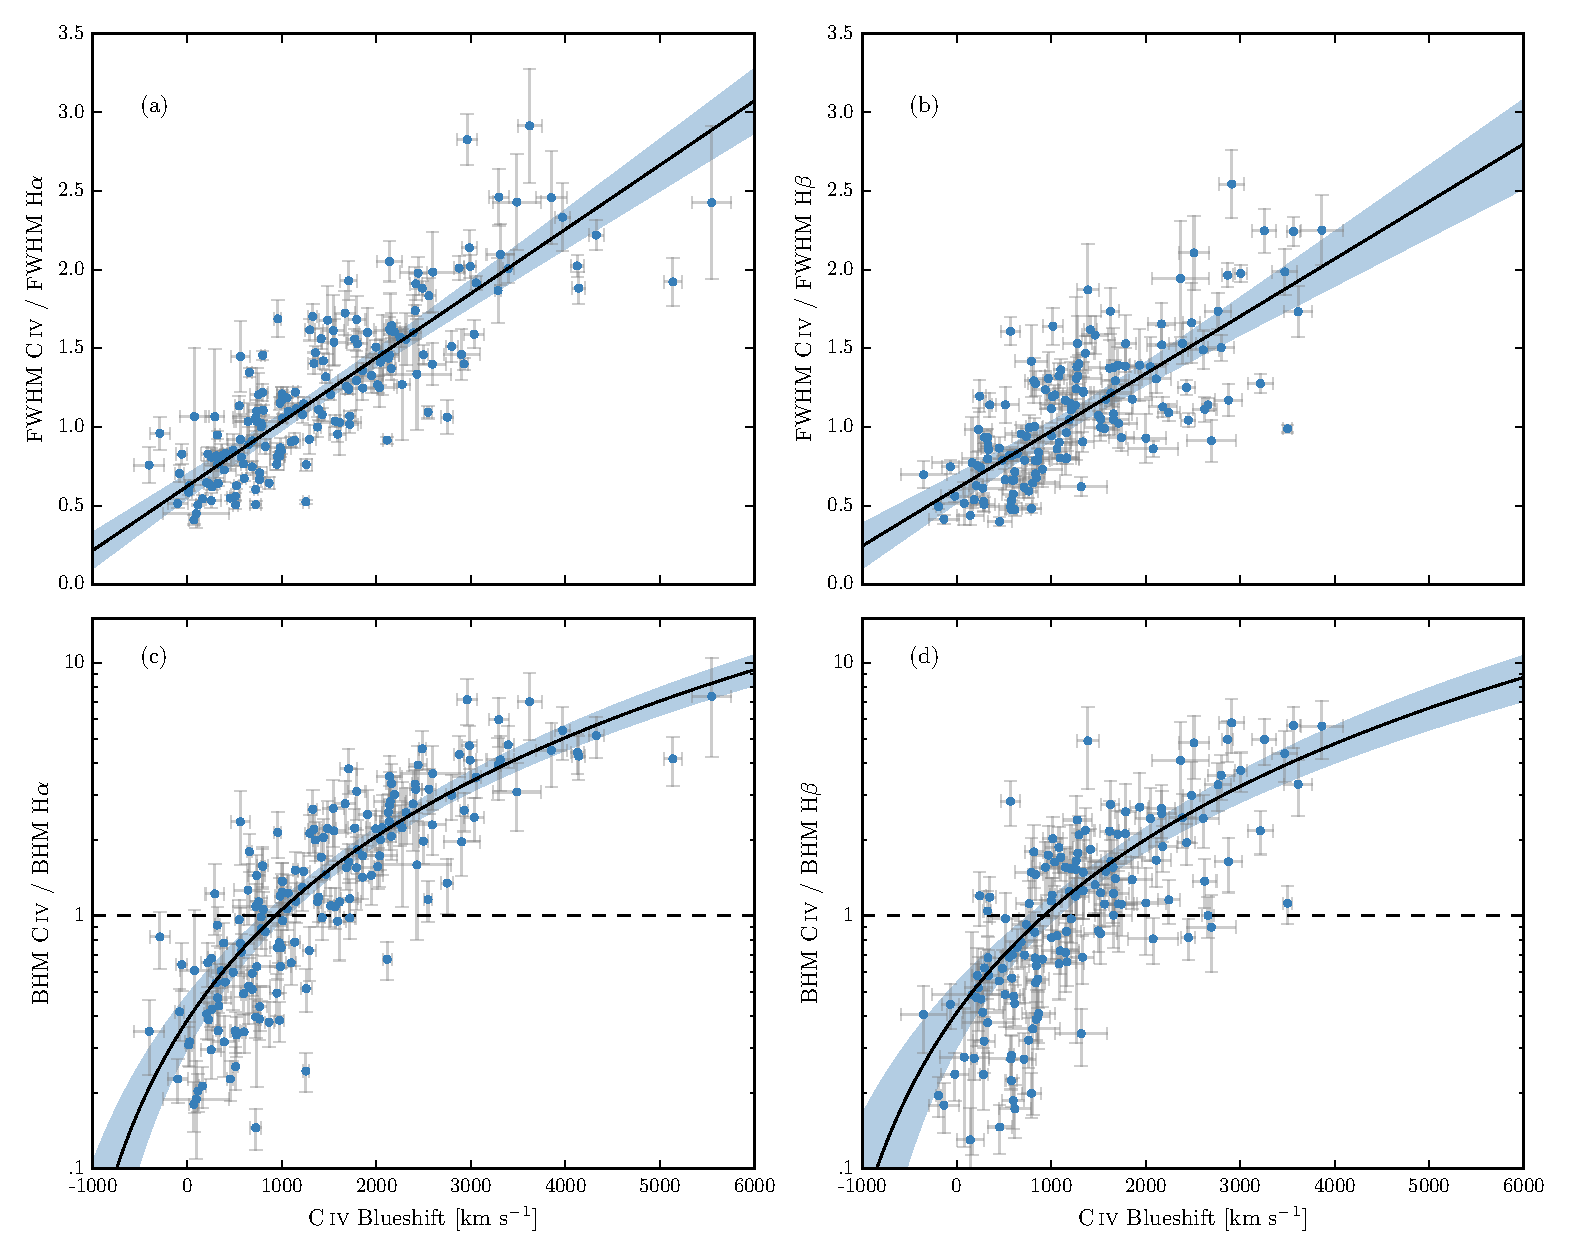
\includegraphics[width=2\columnwidth]{figures/chapter03/fwhm_and_bhm.pdf} 
    \caption{\ion{C}{IV} FWHM relative to \ha FWHM (a) and \hb FWHM (b), and \ion{C}{IV} based BH mass (BHM) compared to \ha based mass (c) and \hb based mass (d), all as a function of the \ion{C}{IV} blueshift. The black line is our best-fit linear model, and the shaded region shows the 2-$\sigma$ uncertainties on the slope and intercept. The \ha FWHM have been scaled to match the \hb FWHM using Eq.~\ref{eq:ha2hb}.}  
    \label{fig:correction}
\end{figure*}

In Fig.~\ref{fig:mcmc_parameters} we show the one- and two-dimensional projections of the posterior distribution from the linear fit to the FWHM \ion{C}{IV}/\ha ratio. 
The projections from the FWHM \ion{C}{IV}/\hb fit (not shown) have very similar appearances.
In Fig.~\ref{fig:correction}a we plot the maximum likelihood model and the 2$\sigma$ uncertainties on the model parameters. 
The maximum likelihood line is given by  

\begin{equation}
    \label{eq:hafwhm}
    \rm{FWHM}(\rm{C}\,\textsc{iv}, \rm{Corr.}) = \frac{\rm{FWHM}(\rm{C}\,\textsc{iv}, \rm{Meas.})}{ (0.41\pm0.02) \left(\frac{\rm{C}\,\textsc{iv}\, Blueshift}{10^3 {\rm \,km\,s^{-1}}} \right) + (0.62\pm0.04)}
\end{equation}

\noindent for the \ion{C}{IV}/\ha fit and 

\begin{equation}
    \label{eq:hbfwhm}
    \rm{FWHM}(\rm{C}\,\textsc{iv}, \rm{Corr.}) = \frac{\rm{FWHM}(\rm{C}\,\textsc{iv}, \rm{Meas.})}{ (0.36\pm0.03) \left(\frac{\rm{C}\,\textsc{iv}\, Blueshift}{10^3 {\rm \,km\,s^{-1}}} \right) + (0.61\pm0.04)}
\end{equation}

\noindent for the \ion{C}{IV}/\hb fit. 
The intercepts of the two relations are consistent, while the difference between the slopes is only marginally inconsistent given the quoted uncertainties. 

The intrinsic scatter in the data about the linear relation we infer is $0.23 \pm 0.02$ and $0.25 \pm 0.02$ for the \ha and \hb fits respectively. 
The intrinsic scatter for the \ha fit is represented by the Normal probability density distribution shown in Fig.~\ref{fig:intrinsic_scatter}. 
In the same figure we show the distribution of the orthogonal displacement of each data point from the best-fitting linear relationship. 
The two distributions are well-matched, which demonstrates that our model is a good representation of the data and the measurement errors on the data points are small relative to the intrinsic scatter.    

The overall (intrinsic and measurement) scatter about the best-fitting model is slightly higher when the \ion{C}{IV} line-widths are compared to \hb (0.12 dex) than when compared to \ha (0.10 dex). 
This is likely due, at least in part, to the generally higher S/N of the \ha emission. 
In addition, contributions from the strong [\ion{O}{III}] doublet in the vicinity of \hb make de-blending the \hb emission more uncertain. 
As a consequence, for quasars where \ha and \hb are both measured, the mean uncertainty on the \ha FWHM is 130\kms, compared to 340\kms for \hbns. 

In the next section we use both the \ha and \hb lines to calculate unbiased BH masses. 
We use the \ha measurements to derive an empirical \ion{C}{IV} blueshift based correction to the \ion{C}{IV} masses (Eq.~\ref{eq:masscorrection}) because of the issues related to the accurate modelling of the \hbns-profile just described.  
An extra advantage, which is evident in Fig.~\ref{fig:correction}, is that the \ha sample has a better \ion{C}{IV} blueshift coverage. 
However, as can be seen from the similarity of Equations \ref{eq:hafwhm} and \ref{eq:hbfwhm}, our results would not change significantly were we instead to use the \hb sample. 

\begin{figure}
    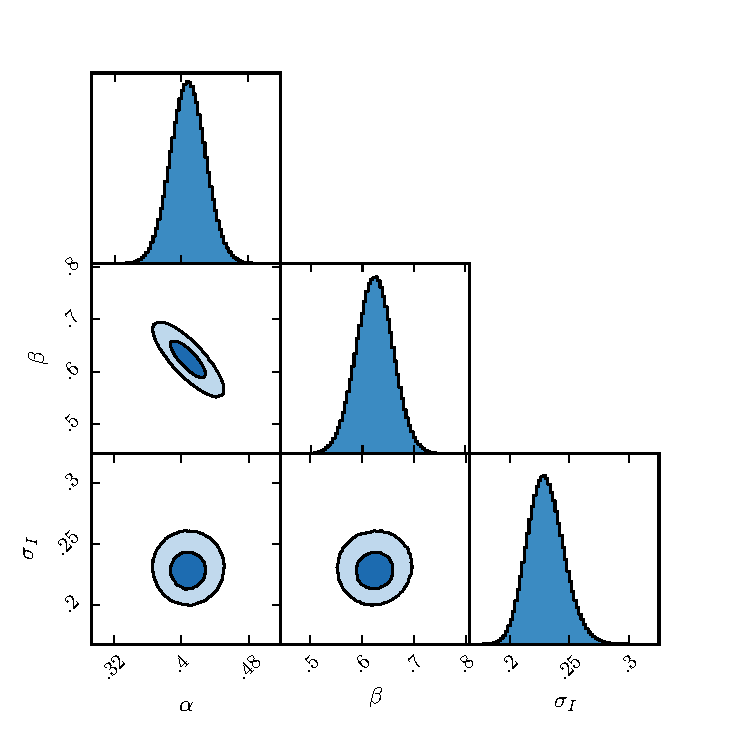
\includegraphics[width=\columnwidth]{figures/chapter03/civ_ha_mcmc_parameters.pdf} 
    \caption{One- and two-dimensional projections of the MCMC sample of the posterior distribution for a linear fit to the FWHM \ion{C}{IV}/\ha ratio as a function of the \ion{C}{IV} blueshift. In the two-dimensional projections we show 1- and 2-$\sigma$ contours. The posterior distribution for the linear fit to the FWHM \ion{C}{IV}/\hb ratio, which we do not show, has a very similar appearance.} 
    \label{fig:mcmc_parameters}
\end{figure}

\begin{figure}
    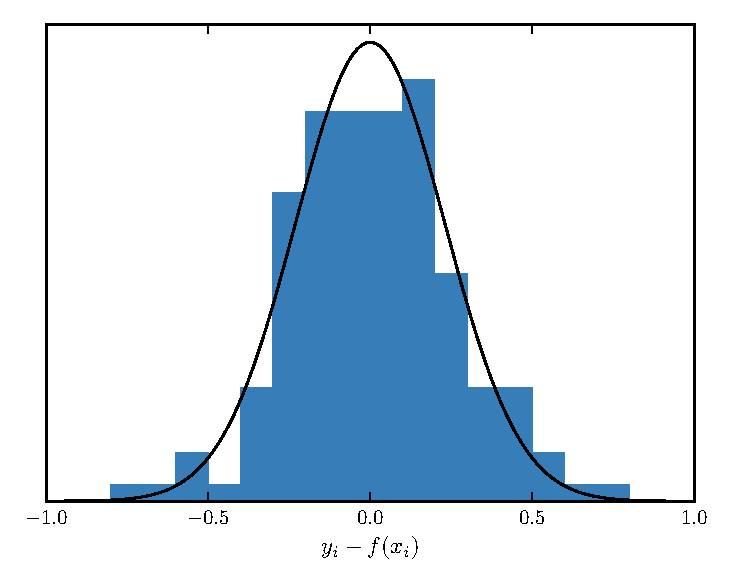
\includegraphics[width=\columnwidth]{figures/chapter03/intrinsic_scatter.pdf} 
    \caption{The distribution of the orthogonal displacement of each data point from the best-fitting linear relationship in the fit to FWHM(\ion{C}{IV})/FWHM(\hans) as a function of the \ion{C}{IV} blueshift (blue histogram). The black curve is a Normal distribution with a width equal to the intrinsic scatter in the population inferred from the fit. The two distributions are well-matched, which demonstrates that our model is a good representation of the data and the measurement errors on the data points are small relative to the intrinsic scatter.} 
    \label{fig:intrinsic_scatter}
\end{figure}

\subsection{\ion{C}{IV} based virial BH mass estimates}

We calculate virial BH mass estimates from \ion{C}{IV}, \ha and \hb using the widely-adopted \citet{vestergaard06} scaling relations (their equations 5 and 7 for \hans/\hb and \ion{C}{IV} respectively). 
In Figs.~\ref{fig:correction}c and d the \ion{C}{IV}-based estimates are compared to the \hans/\hb estimates as a function of the \ion{C}{IV} blueshift. 
There is a strong systematic error in the \ion{C}{IV}-based masses as a function of blueshift, which is a direct consequence of the FWHM trend described in the previous section. 
The \ion{C}{IV} emission-based BH-masses are in error by a factor of more than five at 3000\kms in \ion{C}{IV} emission blueshift and the overestimate of the BH-masses reaches a factor of 10 for quasars exhibiting the most extreme blueshifts, $\gtrsim$5000\kms. 

The virial product is the product of the virial velocity squared and the BLR radius \citep[e.g.][]{shen13}, and is proportional to the BH mass. 
We use the corrected \ion{C}{IV} FWHM given by Eq.~\ref{eq:hafwhm} as an indicator of the virial velocity, and adopt the same $R-L$ relation for the 1350\,\AA\, continuum luminosity as \citet{vestergaard06} (i.e. $R \propto L^{0.53}$). 
To find the constant scaling factor necessary to transform the virial product in to a BH mass we compute the inverse-variance weighted mean difference between the virial products and the \hans-based masses. 
The virial BH mass can then be expressed in terms of the corrected \ion{C}{IV} FWHM and monochromatic continuum luminosity at 1350\,\AA

\begin{equation}
  \label{eq:masscorrection}
  {\rm MBH}(\rm{C}\,\textsc{iv}, \rm{Corr.}) = 10^{6.71}\left( \frac{\rm{FWHM}(\rm{C}\,\textsc{iv}, \rm{Corr.})}{10^3 {\rm \,km\,s^{-1}}} \right)^2 \left( \frac{\lambda {\rm L}_{\lambda} (1350 \text{\AA}) }{10^{44} {\rm \,erg\,s^{-1}}}  \right)^{0.53}
\end{equation}

Given measured \ion{C}{IV} emission line FWHM and blueshift, equations 4 and 6 can then be used to provide an unbiased estimate of the quasar BH mass.

\section{Practical application of the \ion{C}{IV}-based correction to virial BH-mass estimates}

\subsection{Recipe for unbiased \ion{C}{IV} based BH masses}
\label{sec:recipe}

Equations 4 and 6 together provide an un-biased estimate of the virial BH mass given the FWHM and blueshift of \ion{C}{IV}, together with the continuum luminosity at 1350\,\AA. 
The FWHM is readily obtained, either directly from the data, or, via the fitting of a parametric model to the \ion{C}{IV}-emission line. 
The blueshift -- defined as the bisector of the cumulative line flux -- is also straightforward to measure and our preferred procedure is described in Section~\ref{sec:civ}.
The only potential complication arises in establishing the quasar systemic redshift and hence defining the zero-point for the \ion{C}{IV}-blueshift measurement, since both the blueshift and the systemic redshift cannot be determined from \ion{C}{IV} alone. 
In practice, when rest-frame optical lines are accessible, as is the case for the quasar sample here, an accurate systemic redshift can be obtained. 
The [\ion{O}{III}] doublet and the Balmer lines all have velocity centroids very close to systemic, and the same is true for the broad \ion{Mg}{II} doublet. 
For quasars at very high redshifts, $z\sim6$, systemic redshifts can also be derived using the [\ion{C}{II}] 158 $\mu$m emission in the sub-millimetre band \citep[e.g.][]{venemans16}. 
However, in general, for example in determining the BH-masses of quasars at redshifts $z>2$, if only the rest-frame ultraviolet region is available determining a reliable systemic redshift is non-trivial. 

\citet{shen16b} and our own work shows that there is an intrinsic variation of $\sigma$$\simeq$220\kms in the velocity centroids of the broad-line region relative to a systemic-frame defined by the quasar narrow-line regions. 
As we showed in Paper I, the SDSS DR7 pipeline redshifts are not sufficiently reliable to measure the \ion{C}{IV} blueshift accurately because, in part, the \ion{C}{IV} emission line itself contributes to the determination of the quasar redshifts (see figure 1 in Paper I).
The redshift-determination scheme of \citet{hewett10} provided much improved redshifts for the SDSS DR7 quasar catalogue, not least because the redshift estimates for the majority of quasars were derived using emission-lines other than the \ion{C}{IV}-line itself.
The redshifts for quasars in the SDSS DR10 and DR12 catalogues \citep{paris14,paris17} possess errors of $\simeq$500-750\kms \citep{paris12, font-ribera13}. The impact of low spectrum S/N for fainter quasars in all the SDSS data releases increases the uncertainty further. 
Table~\ref{tab:bhm_error} includes the values for the fractional error in the corrected BH-mass that result from a given error in the determination of the systemic rest-frame. 
For example, the fractional error in the corrected BH mass is 0.39 for a quasar with a 1000\kms\, \ion{C}{IV} blueshift when there is a 500\kms\, uncertainty in the quasar systemic redshift.   

Of potentially more significance for studies of BH-masses as a function of quasar and host-galaxy properties are redshift errors that depend on the form of the quasar ultraviolet SED.
The redshifts from \citet{hewett10} still suffer from systematic errors that are correlated with the shape, and particularly the blueshift, of the \ion{C}{IV} emission line.
For the \citet{hewett10} redshifts, and ultraviolet emission-line based redshifts in general, quasars with large \ion{C}{IV} EW and modest blueshifts have relatively small ($\simeq$300\kms) SED-dependent redshift errors.
Redshift uncertainties as large as $\simeq$1000\kms for such quasars are unusual and the large relative error in the corrected \ion{C}{IV} BH-mass given in Table~\ref{tab:bhm_error} is pessimistic. 

Conversely, systematic redshift errors are greatest for quasars with large blueshifts, reaching $\sim$750\kms in the extreme for the \citet{hewett10} values. The associated error in the corrected \ion{C}{IV} BH-masses is, however, mitigated somewhat due to the smaller gradient of the MBH(\ion{C}{IV})/MBH(Balmer) relation at large \ion{C}{IV} blueshift (see Fig.~\ref{fig:correction}).
A definitive quantification of any systematic SED-dependent errors present in the quasar redshifts contained in the SDSS DR12 catalogue is not yet available but the principal component analysis (PCA) based redshift estimates are expected to be largely free of SED-dependent systematics. 
Given the importance of generating more accurate redshifts for the SDSS DR7 and DR12 quasar samples we will publish a catalogue of more accurate redshifts in due course (see Section~\ref{sec:conclusions}).

\begin{table}
  \centering
  \caption{The fractional error on the corrected BH mass as a function of \ion{C}{IV} blueshift for different uncertainties in the quasar systemic redshift.}
  \label{tab:bhm_error}
  \centering
    \begin{tabular}{ccccc} 
    \hline
    \multirow{1}{*}{} & \multicolumn{4}{c}{\ion{C}{IV} blueshift (\kms) } \\
    \multicolumn{1}{c}{$\delta$v (\kms)} & 
    \multicolumn{1}{c}{0} &
    \multicolumn{1}{c}{1000} &
    \multicolumn{1}{c}{2000} &
    \multicolumn{1}{c}{4000}  \\
    \hline
    250 & 0.33 &  0.20 &  0.14 & 0.09 \\
    500 & 0.65 & 0.39 & 0.28 & 0.18 \\
    1000 &1.30 & 0.79 & 0.57 & 0.36 \\
    \hline
    \end{tabular}
\end{table}

\subsection{Systematic trends in residuals}

The scatter about the best-fitting line in the \ion{C}{IV}/\ha FWHM versus \ion{C}{IV}-blueshift relation is $\sim$0.1 dex, an order of magnitude smaller than the size of the \ion{C}{IV}-blueshift dependent systematic but, nevertheless, still significant.
With a view to reducing the scatter further, we searched for measurable parameters which correlate with the scatter at fixed \ion{C}{IV} blueshift, including the luminosity, redshift, [\ion{O}{III}] equivalent width (EW), and \ion{Fe}{II} EW.
The only significant correlation we find is with the \ha FWHM (Fig.~\ref{fig:residuals_ha_fwhm}).
Quasars with broad \ha lines tend to lie below the relation while quasars with narrow \ha tend to lie above it.
One possibility is that this correlation is simply due to random scatter (either intrinsic or measurement error) in the \ha FWHM which, with the other quasar properties fixed, would naturally produce a correlation between FWHM(\ion{C}{IV})/FWHM(\hans) and FWHM(\hans).
However, the fact that we see no such correlation between the model residuals and the \ion{C}{IV} FWHM suggests that the \ha FWHM correlation could be revealing somthing more fundamental. 
The \hans/\hb FWHM is part of `eigenvector 1' (EV1), the first eigenvector in a principal component analysis which originated from the work of \citet{boroson92}.    
While a number of parameters have been considered within the EV1 context \citep[e.g.][]{brotherton99},
Fig.~\ref{fig:residuals_ha_fwhm} suggests that part of the scatter between the Balmer and \ion{C}{IV} velocity widths might be attributed to differences in the spectral properties which are correlated with EV1 \citep{marziani13}. 

The residuals and the \ha FWHM also correlate with the shape of the line \citep[FWHM/$\sigma$, where $\sigma$ is the dispersion, derived from the second moment velocity; e.g.][]{kollatschny11,Kollatschny13}. 
The narrow lines are, on average, `peakier' (with FWHM/$\sigma\simeq$ 1) than the broader lines (with FWHM/$\sigma\simeq$ 2).   
The origin of the Balmer-line shape correlation is not clear but one possibility is an orientation-dependence of the \ha FWHM \citep[e.g.][]{shen14}. 
In this scenario quasars with broader emission lines are more likely to be in an edge-on orientation relative to our line of sight.  
    
At radio wavelengths, the morphology of the radio structure, parametrized in terms of `core dominance' is believed, at least in a statistical sense, to be a proxy for the orientation of the accretion disk \citep[e.g.][]{jackson91}.
We matched our sample to the FIRST radio catalogue \citep{white97} in an attempt to identify orientation-dependent signatures.  
Following \citet{shen11}, we classified quasars with matches within 5\,arcseconds as core-dominated, while, if multiple matches were found within 30 arcseconds, quasars were classified as lobe-dominated. 
Twenty core- quasars and six lobe-dominated quasars resulted but no statistically significant differences in the \ha line-widths of the two samples were found. 
It should be noted that the sub-sample of radio-detected quasars is small and the effectiveness of the test is further compromised by the lack of radio-detected quasars at large blueshifts \citep[see figure 14 of][for example]{richards11}.

There are currently very few reverberation-mapping measurements of quasars with large \ion{C}{IV} blueshifts.
Looking to the future, the results of the large on-going statistical reverberation mapping projects \citep[e.g.][]{shen15,kingoz15} for luminous quasars at high-redshift will shed new light on the Balmer line emitting region of the BLR for quasars with a range of \ion{C}{IV} blueshifts and lead to a greater understanding of the relation between the Balmer line profile and the BH mass. 

\begin{figure}
    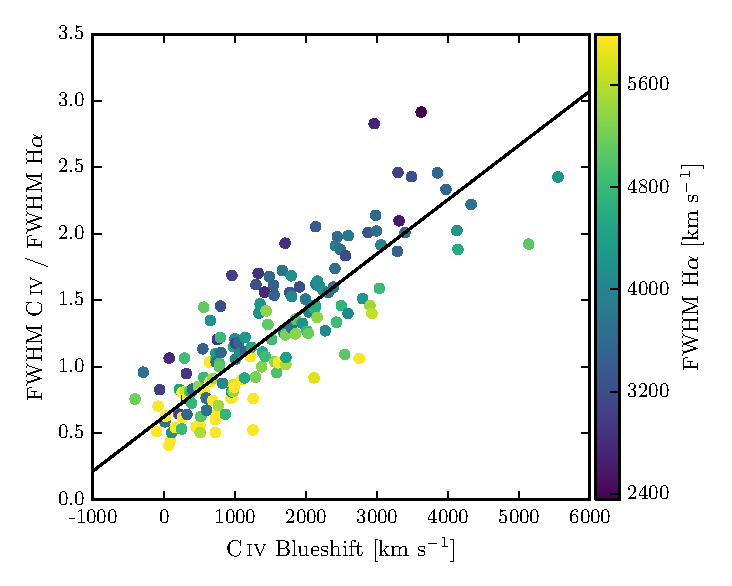
\includegraphics[width=\columnwidth]{figures/chapter03/fwhm_correction_color.pdf}  
    \caption{Same as Fig.~\ref{fig:correction}a, with the marker colour representing the \ha FWHM. At fixed \ion{C}{IV} blueshift, there is a clear \ha FWHM dependent systematic in the model residuals.}   
    \label{fig:residuals_ha_fwhm}
\end{figure}

\subsection{Effectiveness of the \ion{C}{IV} blueshift based correction to BH masses}
\label{sec:effectiveness}

\begin{figure}
    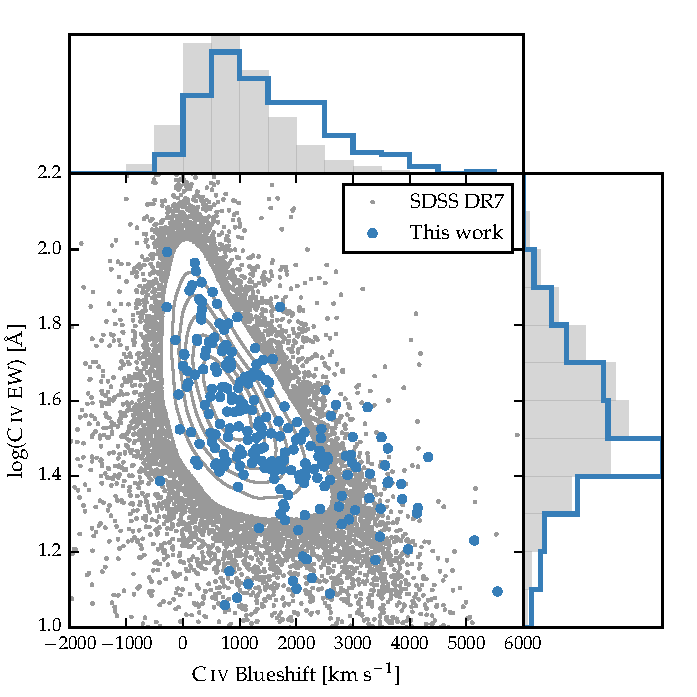
\includegraphics[width=\columnwidth]{figures/chapter03/civ_space.pdf} 
    \caption{Rest-frame EW versus blueshift of the broad \ion{C}{IV}-emission line for 32,157 SDSS DR7 quasars at $1.6 < z < 3.0$ ({\it grey}) and our sample ({\it blue}). For the SDSS quasars, the systemic redshifts used to calculate the blueshifts are from \citet{hewett10} and \ion{C}{IV} emission properties are decribed in Paper I. In regions of high point-density, contours show equally-spaced lines of constant probability density generated using a Gaussian kernel-density estimator. Our sample has very good coverage; the shift to high blueshifts is a result of the high luminosity of our sample in relation to the SDSS sample and the correlation between luminosity and blueshift.} 
    \label{fig:civ_space}
\end{figure}

Figure~\ref{fig:civ_space} demonstrates that our sample has an excellent coverage of the EW-blueshift parameter space in relation to SDSS DR7 quasars at redshifts $1.6 < z < 3.0$. 
The systematic offset to higher \ion{C}{IV} blueshifts for our catalogue relative to the SDSS quasars as a whole is a result of the higher mean luminosity relative to the SDSS sample (Fig.~\ref{fig:lzplane}).
Our sample includes 21 quasars with \ion{C}{IV} blueshifts $>$3000\kms, and extends to $\sim$5000\kms, i.e. at the very extreme of what is observed in this redshift and luminosity range. 
Our investigation thus demonstrates that the \ion{C}{IV}-blueshift based correction derived in this paper is applicable to very high blueshifts. 
Conversely, there are no quasars in our catalogue with \ion{C}{IV} blueshifts $\lesssim$0\kms and we caution against extrapolating the correction formula to negative blueshifts. 

\begin{figure}
    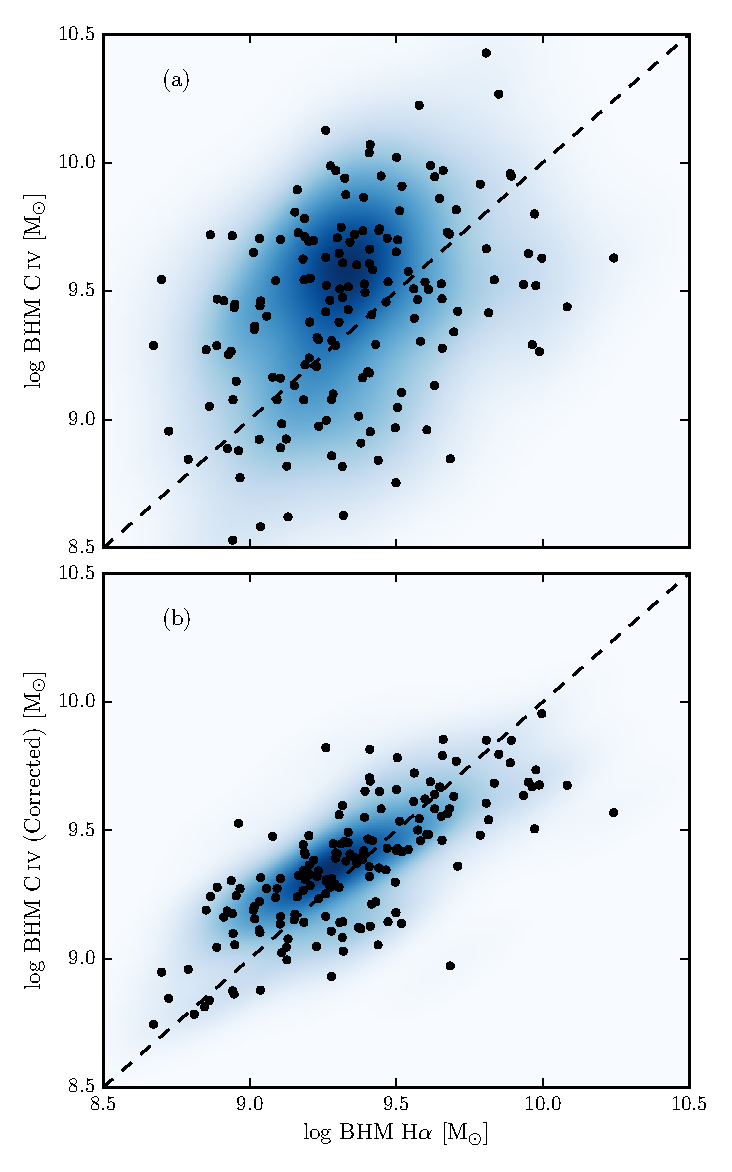
\includegraphics[width=\columnwidth]{figures/chapter03/bhm_comparison.pdf} 
    \caption{Comparison of the \ion{C}{IV}- and \hans-based BH masses before (a) and after (b) applying the \ion{C}{IV} blueshift-based correction to the \ion{C}{IV} FWHM. The density of the plotted points (estimated using a Gaussian kernel density estimator) is represented by the colour. The correction to the \ion{C}{IV} BH masses decreases the scatter by from 0.4 to 0.2 dex.}   
    \label{fig:bhm_comparison}
\end{figure}

Figure~\ref{fig:bhm_comparison} compares the \ion{C}{IV}- and \hans-based BH masses before and after applying the blueshift-based correction to the \ion{C}{IV} FWHM.
Before the correction, the correlation between the \ion{C}{IV}- and \hans-based BH masses is very weak, and the scatter between the masses is 0.4 dex. 
After correcting the \ion{C}{IV} FWHM for the non-virial contribution, the correlation improves dramatically. 
The scatter between the corrected \ion{C}{IV}-based masses and the \hans-based masses is reduced to 0.2 dex. 
The scatter is 0.24 dex at low \ion{C}{IV} blueshifts ($\sim$0\kms) and 0.10 dex at high blueshifts ($\sim$3000\kms). 

\begin{figure}
    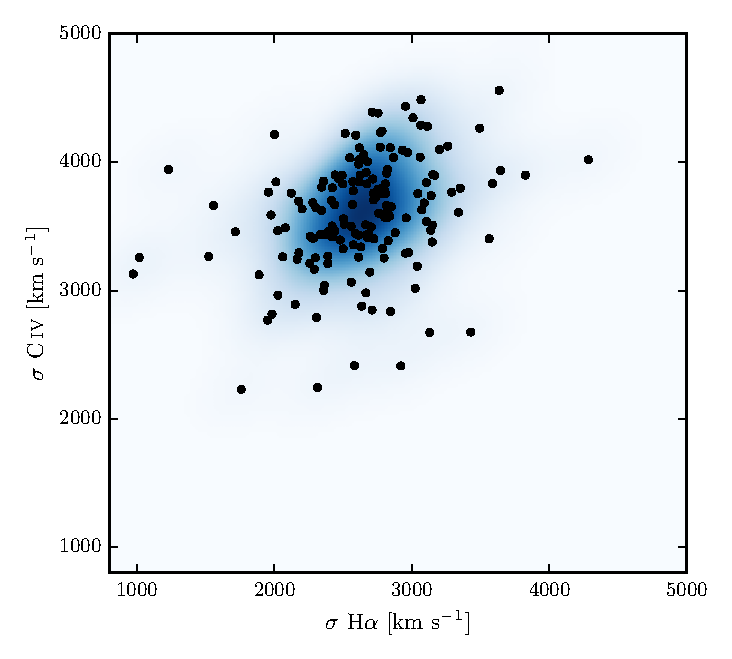
\includegraphics[width=\columnwidth]{figures/chapter03/dispersion_comparison.pdf} 
    \caption{Comparison of the \ion{C}{IV} and \ha line dispersion, $\sigma$. The density of the plotted points (estimated using a Gaussian kernel density estimator) is represented by the colour. Estimating a reliable BH mass from the \ion{C}{IV} FWHM and blueshift line is substantially more effective than using the \ion{C}{IV} line dispersion with, or without, the line blueshift. The \ion{C}{IV} dispersion values are larger than the corresponding \ha measurements by a factor of 1.4 on average, which is consistent with reverberation mapping measurements \citep{vestergaard06}.} 
    \label{fig:dispersion_comparison}
\end{figure}

There has been a considerable amount of attention regarding the relative merits of using the FWHM or dispersion to characterise the velocity width \citep[e.g.][]{denney13}.
As we showed in Paper I, the line dispersion is relatively insensitive to the blueshift and shape of the \ion{C}{IV} line. 
Therefore, without the blueshift information, using the line dispersion would yield a more accurate BH mass than the FWHM (Fig.~\ref{fig:dispersion_comparison}). 
The correlation between the \ha and \ion{C}{IV} line dispersion is, however, weak. 
The Pearson coefficient for the correlation is 0.36 (and just 0.15 when the \hb measurements are used in place of \hans). 
Furthermore, there is little dynamic range in the line dispersion: the scatter is just 480 and 460\kms for \ha and \ion{C}{IV} respectively. The observation suggests that the line dispersion does not fully trace the dynamic range in BH mass present in the quasar population. 
At least part of the reason is that the line dispersion is difficult to measure reliably in current survey-quality data, particularly because of the sensitivity to flux ascribed to the wings of the emission line \citep[e.g.][]{mejia-restrepo16}. 
Figures~\ref{fig:bhm_comparison} and \ref{fig:dispersion_comparison} demonstrate that estimating a reliable BH mass from the \ion{C}{IV} FWHM and blueshift line is substantially more effective than using the \ion{C}{IV} line dispersion with, or without, the line blueshift. 

\subsection{Comparison to previous prescriptions}

\begin{figure*}
    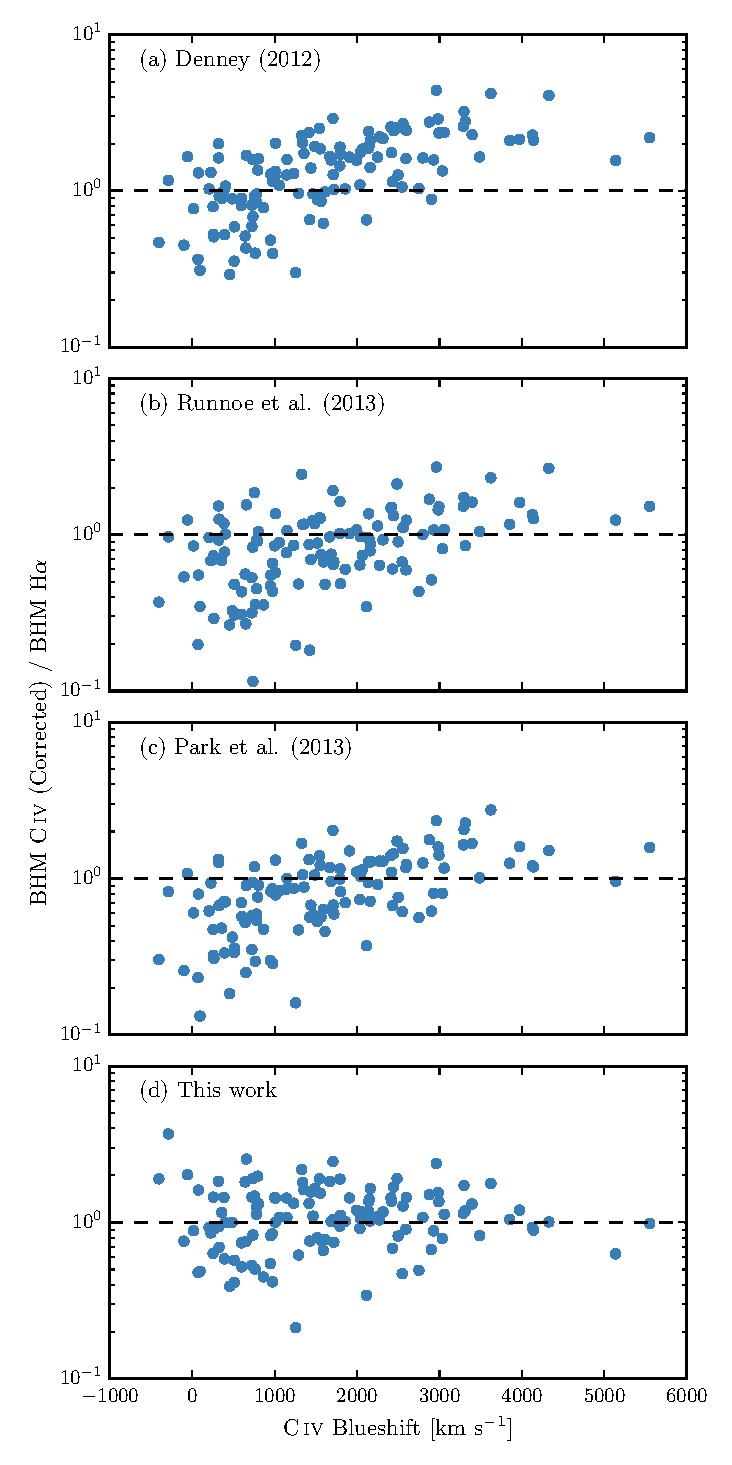
\includegraphics[width=2\columnwidth]{figures/chapter03/corrections.pdf}  
    \caption{Comparison of BH mass estimates derived from \ion{C}{IV} and \ha as a function of the \ion{C}{IV} blueshift. Corrections to the \ion{C}{IV}-based masses have been applied based on the shape (FWHM/$\sigma$) of the \ion{C}{IV} emission line \citep[a;][]{denney12}, the peak flux ratio of the \ion{Si}{IV}+\ion{O}{IV} blend relative to \ion{C}{IV} \citep[b;][]{runnoe13}, by significantly reducing the dependence of the derived BH mass on the \ion{C}{IV} velocity-width \citep[c;][]{park13}, and based on the \ion{C}{IV} blueshift (d; this paper).}
    \label{fig:compare_corrections}
\end{figure*}

In Fig.~\ref{fig:compare_corrections} we compare the \ion{C}{IV} blueshift-based correction presented in this paper to various prescriptions which have been proposed in the literature to derive BH masses from the \ion{C}{IV} line which are consistent with the masses derived from the Balmer lines. 
In each case we compare the corrected \ion{C}{IV}-based masses to the \hans-based masses as a function of the \ion{C}{IV} blueshift. 
The correction proposed by \citet{runnoe13} is based on the spectral region at rest-frame wavelengths of $\sim$1400\,\AA \ (see below). 
Therefore, our analysis is based on the 123 quasars which satisfy this requirement. 

In Fig~\ref{fig:compare_corrections}a the \ion{C}{IV} BH masses have been corrected using the \ion{C}{IV} shape (FWHM/$\sigma$) based correction proposed by \citet{denney12}. 
The correction is not applicable at large \ion{C}{IV} blueshifts, since it was calibrated on a sample of low-luminosity AGN which does not include any such objects.
Therefore, while the consistency between the \hans- and \ion{C}{IV}-based masses at low \ion{C}{IV} blueshifts is improved, at high \ion{C}{IV} blueshifts the \ion{C}{IV}-based masses remain seriously overestimated.

\citet{runnoe13} used the continuum-subtracted peak flux ratio of the ultraviolet emission-line blend of \ion{Si}{IV}+\ion{O}{IV} (at 1400\,\AA) relative to \ion{C}{IV} to correct for non-virial contributions to the \ion{C}{IV} velocity-width. 
Following \citet{runnoe13}, we measure the peak flux by fitting a model with four Gaussian components (two for each emission line) to the continuum-subtracted flux.
As is evident from Fig.~\ref{fig:civ_space}, a correlation exists between the blueshift and equivalent width of \ion{C}{IV}: \ion{C}{IV} emission which is strongly blueshifted is typically weak. 
The \ion{Si}{IV}+\ion{O}{IV} emission-line blend, however, shows significantly less systematic variation. 
Therefore, the \ion{Si}{IV}+\ion{O}{IV}-based correction is quite effective in practice: the systematic bias in the \ion{C}{IV} BH masses at large \ion{C}{IV} blueshifts is reduced to a factor of $\sim2$ (Fig.~\ref{fig:compare_corrections}b).
However, the \ion{C}{IV} based masses are still systematically overestimated at large \ion{C}{IV} blueshifts. 

In contrast to the widely-used \citet{vestergaard06} \ion{C}{IV}-based virial BH mass calibration, the more recent \citet{park13} calibration significantly reduces the dependence of the derived masses on the emission-line velocity width (from the $V^2$ dependence predicted assuming a virialized BLR to just $V^{0.56}$).
As a consequence, the \ion{C}{IV} based masses of the quasars with large \ion{C}{IV} blueshifts are much reduced (Fig.~\ref{fig:compare_corrections}c).
However, the systematic error in the \ion{C}{IV}-based BH masses as a function of \ion{C}{IV} blueshift remains. 

As a comparison, the \ion{C}{IV}-based masses shown in Fig~\ref{fig:compare_corrections}d have been corrected using to the \ion{C}{IV} blueshift-based procedure presented in this paper. 
No systematic in the BH masses as a function of the \ion{C}{IV} blueshift is evident. 

\section{Conclusions}
\label{sec:conclusions}

The main results of this paper are as follows: 

\begin{itemize}
\item We have analysed the spectra of 230 high-luminosity ($10^{45.5}-10^{48}$\,\ergs), redshift $1.5 < z < 4.0$ quasars for which spectra of the Balmer emission lines and the \ion{C}{IV} emission line exist.
The large number of quasars in our spectroscopic catalogue and the wide range in \ion{C}{IV} blueshifts the quasars possess has allowed us to directly investigate biases in \ion{C}{IV}-based BH mass estimates which stem from non-virial contributions to the \ion{C}{IV} emission as a function of the \ion{C}{IV} blueshift, which, in turn, depends directly on the form of the quasar ultraviolet SEDs \citep{richards11}.
\item The \ion{C}{IV} emission-based BH-masses are systematically in error by a factor of more than five at 3000\kms in \ion{C}{IV} emission blueshift and the overestimate of the BH-masses reaches a factor of 10 for quasars exhibiting the most extreme blueshifts, $\gtrsim$5000\kms. 
\item We have derived an empirical correction formula for BH-mass estimates based on the \ion{C}{IV} emission line FWHM and blueshift.
The correction may be applied using equations 4 and 6 in Section~\ref{sec:correction}.
The large SED-dependent systematic error in \ion{C}{IV}-based BH-masses is removed using the correction formulae.
The remaining scatter between the corrected \ion{C}{IV}-based masses and the \hans-based masses is 0.24 dex at low \ion{C}{IV} blueshifts ($\sim$0\kms) and 0.10 dex at high blueshifts ($\sim$3000\kms). 
This is a significant improvement on the 0.40 dex scatter observed between the un-corrected \ion{C}{IV} and \ha BH masses. 
The correction depends only on the \ion{C}{IV} line properties - i.e. the FWHM and blueshift - and allows single-epoch virial BH mass estimates to be made from optical spectra, such as those provided by the SDSS, out to redshifts exceeding $z\sim 5$. 
\end{itemize}

As discussed in Section~\ref{sec:recipe}, uncertainties in redshift estimation and hence the definition of the systemic rest-frame for quasars impact on the accuracy of the corrected BH-masses.
Using published redshift estimates, notably those from \citet{hewett10} for the SDSS DR7 quasars and the BOSS PCA-based redshifts from \citet{paris17} for SDSS DR12, the correction formula given in Section~\ref{sec:correction} produces significant improvements to \ion{C}{IV}-based BH mass estimates.
In a forthcoming work, Allen \& Hewett (in preparation) will present a new redshift-estimation algorithm that produces redshifts independent of the \ion{C}{IV} blueshift and other variations in the ultraviolet SEDs of luminous quasars.
Allen \& Hewett will publish improved redshifts for all quasars in the SDSS DR7 and DR12 which will reduce SED-dependent systematic errors below the apparent inherent dispersion of $\simeq220$\kms associated with broad emission line redshifts \citep{shen16b}.
At the same time we will publish catalogues of unbiased BH masses for both SDSS DR7 and DR12 based on the Allen \& Hewett redshifts. 
The components from the mean-field independent component analysis \citep[see][for an application to astronomical spectra]{allen13} used in the Allen \& Hewett redshift algorithm will also be published.
With these components, if a rest-frame ultraviolet spectrum is available, it will be straightforward to determine the systemic redshift, via a simple optimisation procedure, and hence calculate the \ion{C}{IV} blueshift. 

\section{Comparison to Shen}
\label{appendix:shen}

\begin{figure}
    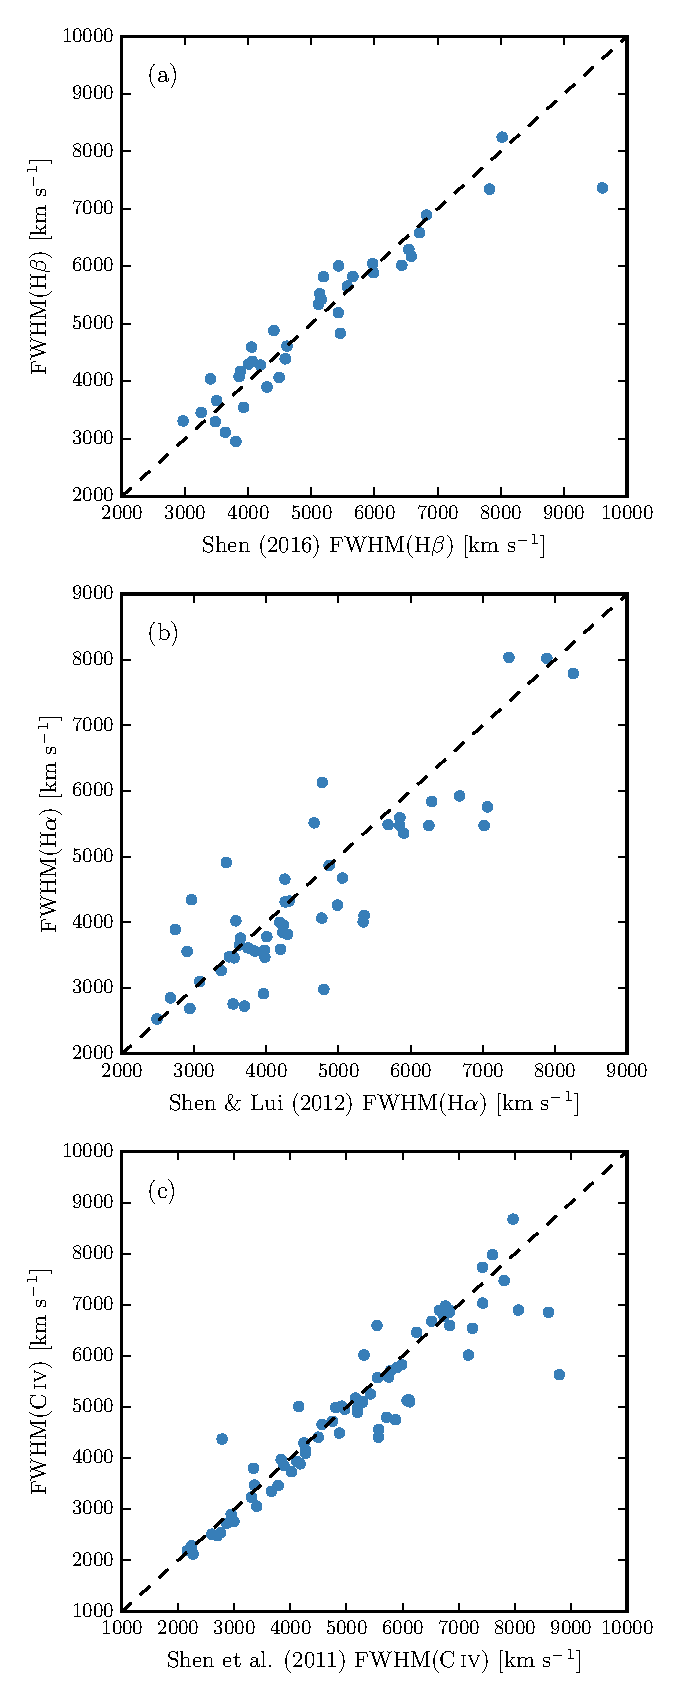
\includegraphics[width=\columnwidth]{figures/chapter03/shen_comparison.pdf} 
    \caption{Demonstration of the effectiveness of our line parameter estimation scheme via a comparison of (a) the \hb FWHM with \citet{shen16a}, (b) the \hb FWHM with \citet{shen12}, and (c) the \ion{C}{IV} FWHM with \citet{shen11}.} 
    \label{fig:shen_comparison}
\end{figure}

In this section we verify the accuracy of our parameter estimation scheme by comparing our FWHM measurements to measurements published in \cite{shen11}, \cite{shen12} and \cite{shen16a}. 

The parametric model we fit to the \hbns/[\ion{O}{III}] emission region was very similar to the model employed by \citet{shen16a}. 
In Fig.~\ref{fig:shen_comparison}a we plot our \hb FWHM measurements against the measurements published in \citet{shen16a}, for 39 quasars in common to both samples. 
As expected, we observe a very tight correlation, with a scatter of 0.04 dex. 

In Fig.~\ref{fig:shen_comparison}b we plot our \ha FWHM measurements against the measurements published in \citet{shen12}, for 51 quasars in common to both samples.
There is a strong correlation and, although the scatter is larger than for the \hb comparison (0.07 dex), no significant systematic bias. 

Finally, in Fig.~\ref{fig:shen_comparison}c we compare our measurements of the \ion{C}{IV} FWHM from the 71 SDSS DR7 spectra in our sample with the measurements published in \citet{shen11}. 
\citet{shen11} fit the \ion{C}{IV} line profile with a composite model comprising up to three Gaussian components, whereas we used (up to order six) Gauss-Hermite polynomials. 
Nevertheless, there is a very strong agreement between our measurements, with a scatter of 0.05 dex. 
%\include{multiToC} % <--- just debug stuff, ignore for your documents
% ********************************************************************
% Backmatter
%*******************************************************
\appendix
%\renewcommand{\thechapter}{\alph{chapter}}
\cleardoublepage
\part{Appendix}
%********************************************************************
% Appendix
%*******************************************************
% If problems with the headers: get headings in appendix etc. right
%\markboth{\spacedlowsmallcaps{Appendix}}{\spacedlowsmallcaps{Appendix}}



%********************************************************************
% Other Stuff in the Back
%*******************************************************
\cleardoublepage%********************************************************************
% Bibliography
%*******************************************************
% work-around to have small caps also here in the headline
\manualmark
\markboth{\spacedlowsmallcaps{\bibname}}{\spacedlowsmallcaps{\bibname}} % work-around to have small caps also
%\phantomsection 
\refstepcounter{dummy}
\addtocontents{toc}{\protect\vspace{\beforebibskip}} % to have the bib a bit from the rest in the toc
\addcontentsline{toc}{chapter}{\tocEntry{\bibname}}
\label{app:bibliography}
\printbibliography

\cleardoublepage% !TEX root = ../thesis.tex

%*******************************************************
% Declaration
%*******************************************************
\refstepcounter{dummy}
\pdfbookmark[0]{Declaration}{declaration}
\chapter*{Declaration}
\thispagestyle{empty}
This dissertation is the result of my own work and includes nothing which is the outcome of work done in collaboration except as declared in the Preface and specified in the text.
It is not substantially the same as any that I have submitted, or, is being concurrently submitted for a degree or diploma or other qualification at the University of Cambridge or any other University or similar institution except as declared in the Preface and specified in the text.
I further state that no substantial part of my dissertation has already been submitted, or, is being concurrently submitted for any such degree, diploma or other qualification at the University of Cambridge or any other University or similar institution except as declared in the Preface and specified in the text.
The use of `we' in the main text is a stylistic choice.

\bigskip
\noindent This thesis has used material from the following publications.
\begin{itemize}
\item Chapters~\ref{ch:nirsample} and \ref{ch:bhmass} use material from \citet{coatman16} and \citet{coatman17}.
\end{itemize}
\bigskip

\begin{flushright}
    \begin{tabular}{m{5cm}}
        \\ \hline
        \centering\myName \\
    \end{tabular}
\end{flushright}
\cleardoublepage\pagestyle{empty}

\hfill

\vfill


\pdfbookmark[0]{Colophon}{colophon}
\section*{Colophon}
This document was typeset using the typographical look-and-feel \texttt{classicthesis} developed by Andr\'e Miede. 
The style was inspired by Robert Bringhurst's seminal book on typography ``\emph{The Elements of Typographic Style}''. 
\texttt{classicthesis} is available for both \LaTeX\ and \mLyX: 
\begin{center}
\url{https://bitbucket.org/amiede/classicthesis/}
\end{center}
Happy users of \texttt{classicthesis} usually send a real postcard to the author, a collection of postcards received so far is featured here: 
\begin{center}
\url{http://postcards.miede.de/}
\end{center}
 
\bigskip

\noindent\finalVersionString

%Hermann Zapf's \emph{Palatino} and \emph{Euler} type faces (Type~1 PostScript fonts \emph{URW
%Palladio L} and \emph{FPL}) are used. The ``typewriter'' text is typeset in \emph{Bera Mono}, 
%originally developed by Bitstream, Inc. as ``Bitstream Vera''. (Type~1 PostScript fonts were made 
%available by Malte Rosenau and
%Ulrich Dirr.)

%\paragraph{note:} The custom size of the textblock was calculated
%using the directions given by Mr. Bringhurst (pages 26--29 and
%175/176). 10~pt Palatino needs  133.21~pt for the string
%``abcdefghijklmnopqrstuvwxyz''. This yields a good line length between
%24--26~pc (288--312~pt). Using a ``\emph{double square textblock}''
%with a 1:2 ratio this results in a textblock of 312:624~pt (which
%includes the headline in this design). A good alternative would be the
%``\emph{golden section textblock}'' with a ratio of 1:1.62, here
%312:505.44~pt. For comparison, \texttt{DIV9} of the \texttt{typearea}
%package results in a line length of 389~pt (32.4~pc), which is by far
%too long. However, this information will only be of interest for
%hardcore pseudo-typographers like me.%
%
%To make your own calculations, use the following commands and look up
%the corresponding lengths in the book:
%\begin{verbatim}
%    \settowidth{\abcd}{abcdefghijklmnopqrstuvwxyz}
%    \the\abcd\ % prints the value of the length
%\end{verbatim}
%Please see the file \texttt{classicthesis.sty} for some precalculated 
%values for Palatino and Minion.
%
%    \settowidth{\abcd}{abcdefghijklmnopqrstuvwxyz}
%    \the\abcd\ % prints the value of the length





% ********************************************************************
% Game Over: Restore, Restart, or Quit?
%*******************************************************
\end{document}
% ********************************************************************
